%%%%%%%%%%%%%%%%%%%%%%%%%
%%  Capítulo 3: Modelado y simulacion de metamateriales  %%
%%%%%%%%%%%%%%%%%%%%%%%%%
\section{Modelos analíticos de estructuras uniplanares de banda prohibida electromagnética}
\label{sec:modelo_analitico}

% buena intro en rahmat (libro), pagina 35-37
% Buscar las distintas formas, incluyendo Peano. Relación con FSS.
% Buena intro esn Goussetis, Feresidis, Vardaxoglou.
% Diseños para incidencia obliucua: Kim, Yand, Elsherbeni. Tambien en Lin, Li, Zhang.
% Hilbert: McVAy, Engheta, Hoorfar.
% Power loss analysis: Mohajer-Iravani, Ramahi, de Hindawi corp.
% Kern, Douglas, Werner.
% Analisis en Goussetis, Feresidis, paper posta. Tipos de resonancia.
% Lamminen, Vimpari, Saily. 
% Maci, Caiazzo, Cucini. Jodido, interesante. Leer.
% Rahmat. Pagina 77 libro.
% Engheta, pagina 290.

% Lightline stuff. Rahmat, pagina 28. Caloz, pagina 139. Pozar pag 386


El análisis de estructuras de banda prohibida electromagnética, así como de superficies selectoras de frecuencia (FSS), se suele realizar a través de simulaciones numéricas de onda completa, utilizando el método de elementos finitos (FEM) o métodos en el dominio del tiempo, como FDTD, dado que permiten la resolución de los problemas de forma tridimensional, lo que habilita al diseñador a conocer el comportamiento de configuraciones de una o más capas, así como los efectos de curvaturas y discontinuidades en la periodicidad. Estos métodos, si bien son flexibles, no otorgan intuición física y resultan computacionalmente demandantes. Análisis de tipo numérico en dos dimensiones han sido propuestos, principalmente utilizando el método de momentos (MOM), a partir de los cuales han surgido otras técnicas de estudio de las estructuras bidimensionales, basadas en la búsqueda de capacidades e inductancias equivalentes, dispuestas de forma tal que la respuesta en frecuencia tenga un comportamiento similar al observado en las simulaciones. Estos métodos, que en ocasiones derivan en aproximaciones de primer orden a elementos circuitales, se denominan semi-analíticos, y se usan especialmente cuando la periodicidad es mucho menor a la longitud de onda incidente. Este tipo de análisis ha permitido la aplicación de otros métodos numéricos, como TMM (\textit{Transmission Matrix Method}) y TLM (\textit{Transmission-Line Matrix Method}), de mayor simplicidad y con suficiente acercamiento al problema físico para que el resultado resulte intuitivo para el diseño preliminar.

Los métodos de modelado orientados a la descripción del comportamiento en el primer modo (en bajas frecuencias) de estructuras de banda prohibida electromagnética bidimensionales no requieren de una simulación numérica de onda completa previa \cite{KimSchuttAine:AnalysisHybrid}. En ellos, como se muestra en la figura \ref{fig:circuito-equivalente-kim-parches}, las inductancias y capacidades surgen del análisis intuitivo y cuasiestático del efecto de cada aspecto de la geometría de la estructura metalodieléctrica de las celdas unitarias. Así, para las celdas de dicha figura, formadas por parches rectangulares unidos por puentes \textit{microstrip}, se debe considerar que cada parche presenta una capacidad contra el plano conductor ($C_p$), dada simplemente como la expresión de capacidad entre placas planas paralelas, y una inductancia $L_p$, dada por:

\begin{align}
\label{eq:Cp_Lp}
C_p &= \frac{\epsilon_r \epsilon_0 b^2}{h} \\
L_p &= \mu_0 h
\end{align}

Los parches cercanos dan lugar a una capacidad ($C_g$) \cite{Marcela:Tesis} \cite{Sievenpiper:Thesis} \cite{KimSchuttAine:AnalysisHybrid}, y los puentes entre parches generan una inductandia ($L_{b}$) \cite{KimSchuttAine:AnalysisHybrid}:

\begin{align}
\label{eq:cgap-y-lgap}
C_{g} = \frac{b \epsilon_0 (1+\epsilon_r)}{\pi} \cosh^{-1} (a / g) \\
L_{b} = 0.2\; \text{nH/mm} \cdot \ln (2\pi \frac{h}{w})
\end{align}

donde $a$ es el tamaño de la celda unitaria, $h$ es el ancho del dieléctrico y $w$ es el ancho del puente. Estos parámetros permiten calcular los valores de $Y$ y $Z$ requeridos para el análisis con líneas de transmisión cargadas, utilizados para calcular los diagramas de dispersión en la sección \ref{sec:diag-de-dispersion}.


\begin{figure}[h]
	\centering
	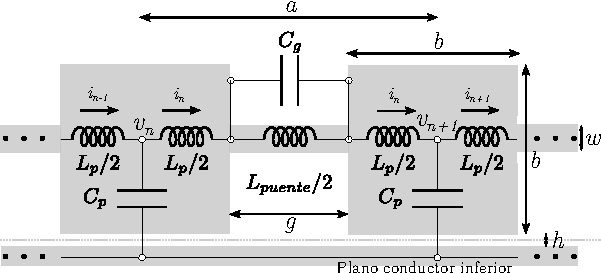
\includegraphics[width=0.9\textwidth]{Fundamentos/circuito-equivalente-celda-unitaria.pdf}
	\caption{Circuito equivalente propuesto para el análisis de primer modo de una celda unitaria bidimensional arbitraria, propuesto por \cite{KimSchuttAine:AnalysisHybrid}.}
	\label{fig:circuito-equivalente-kim-parches}
\end{figure}

%\begin{figure}[htp]
%	\centering
%	\begin{circuitikz} \draw
%		(0,0) -- (1,0)node[midway,scale=2,fill=white]{$\cdots$}
%		-- (9,0) -- (10,0)node[midway,scale=2,fill=white]{$\cdots$}
%		(0,2) -- (1,2)node[midway,scale=2,fill=white]{$\cdots$} 
%		to [L,-o,l_=$L_p/2$] (2.5,2)
%		to [L,o-o,l_=$L_p/2$] (4,2)
%		to [L,o-o,l_=$L_{puente}/2$] (6,2)
%		to [L,o-o,l_=$L_p/2$] (7.5,2)
%		to [L,o-,l_=$L_p/2$] (9,2)
%		-- (10,2)node[midway,scale=2,fill=white]{$\cdots$}
%		(2.5,2) to [C,o-o,l_=$C_p$] (2.5,0)
%		(7.5,2) to [C,o-o,l_=$C_p$] (7.5,0)
%		(4,3) to [C,o-o,l^=$C_g$] (6,3);
%		%			to [C,l=$C'_R \Delta_z$] (7,0)
%		%		-- (9,0) to [L,l_=$L'_L / \Delta_z$] (9,2)
%		%		-- (7,2)
%		%		(9,2) -- (11,2)
%		%		to [R,l=$R / \Delta_z$] (11,0)
%		%		-- (9,0)
%		%		(11,0) -- (12,0) -- (13,0)node[midway,scale=2,fill=white]{$\cdots$}
%		%		(11,2) -- (12,2) -- (13,2)node[midway,scale=2,fill=white]{$\cdots$};
%	\end{circuitikz}  	
%	\caption{Circuito equivalente de porción de línea de transmisión cargada, de longitud $d$.}
%	\label{fig:linea-transm-cargada-periodica}
%\end{figure}

Para el caso unidimensional, resulta sencillo obtener una expresión de la ecuación de dispersión, utilizando un acercamiento circuital, considerando el circuito de la figura \ref{fig:circuito-equivalente-kim-parches}, donde se demarcaron las tensiones y corrientes a considerar, alrededor de una celda unitaria determinada ($n$). A partir del planteo de las ecuaciones circuitales, y considerando que las tensiones y corrientes tienen un comportamiento armónico:

\begin{align}
	v_n - v_{n+1} = i_n \left( \frac{L_p}{2} + \frac{j \omega L_b}{1-\omega^2 L_b C_g} + \frac{L_p}{2} \right) \\
	\frac{i_n - i_{n+1}}{j\omega C_p} = v_n
\end{align}

Reordenando e imponiendo la condición de Bloch-Floquet, que indica, expresado de forma conveniente, que $i_{n+1} = i_{n} e^{-\gamma a}$, y que $v_{n+1} = v_{n} e^{-\gamma a}$:

\begin{align}
	\begin{bmatrix}
		1 & -j \omega C_p \\
		-\frac{L_p}{2} + \frac{j \omega L_b}{1-\omega^2 L_b C_g} + \frac{L_p}{2} & 1
	\end{bmatrix}
	\begin{bmatrix}
		i_n \\
		v_n
	\end{bmatrix}
	=
	\begin{bmatrix}
		i_{n+1} \\
		v_{n+1}
	\end{bmatrix}
	=
	\begin{bmatrix}
		i_n e^{-\gamma a} \\
		v_n e^{-\gamma a}
	\end{bmatrix}
	=
	\begin{bmatrix}
		1 & 0 \\
		0 & 1
	\end{bmatrix}
	\begin{bmatrix}
		i_n e^{-\gamma a} \\
		v_n e^{-\gamma a}
	\end{bmatrix}
\end{align}

Lo que se reduce a:

\begin{align}
	\begin{bmatrix}
		1-e^{-\gamma a} & -j \omega C_p \\
		-\frac{L_p}{2} + \frac{j \omega L_b}{1-\omega^2 L_b C_g} + \frac{L_p}{2} & 1-e^{-\gamma a}
	\end{bmatrix}
	\begin{bmatrix}
		i_n \\
		v_n
	\end{bmatrix}
	=0
\end{align}

Para obtener soluciones más allá de la trivial, el determinante de la matriz debe ser cero, por lo que resulta la ecuación de dispersión:

\begin{align}
	1+e^{-2\gamma a} - 2 e^{-\gamma a} - j \omega C_p L_p - \frac{\omega^2 C_p L_b}{1-\omega^2 L_b C_g} = 0
\end{align}

%POdría poner un gráfico.

Para el caso de las superficies de alta impedancia sin vías de conexión entre la geometría superior y el plano de tierra inferior, Tretyakov y otros (\cite{Tretyakov:AnalyticalModeling}, \cite{Yakovlev:AnalyticalModelingHIS}) han propuesto un análisis centrado en la similitud con las FSS (\textit{Frequency Selective Surfaces}), considerando a las superficies EBG uniplanares como FSS con un plano de tierra. De esta manera es posible utilizar los modelos desarrollados durante el siglo \textsc{XX} para el análisis de las superficies selectoras de frecuencias, en el estudio de EBGs, dado que el comportamiento de banda prohibida se da por el mismo motivo que el comportamiento de filtro de las FSS \cite{Goussetis:TailoringAMCEBGCharacteristics}, relacionado a la frecuencia de resonancia del arreglo de elementos. Para ello, se considera el circuito equivalente de la figura \ref{fig:tretyankov-circuito-equivalente}, donde $Z_g$ es la impedancia que impone la FSS que se dispone sobre el plano dieléctrico, y $Z_d$ es la impedancia del conjunto formado por el dieléctrico y el plano conductor. De esta forma, la impedancia de superficie resulta del paralelo de ambas. La impedancia del conjunto dieléctrico-plano conductor fue analizada en el capítulo anterior, y depende de la polarización (TE o TM). La impedancia que impone el arreglo periódico bidimensional, la FSS, requiere de un análisis particular de cada caso, y los resultados analíticos en la literatura están limitados a arreglos de rectángulos, dipolos y cruces, y sus correspondientes estructuras complementarias.

\begin{figure}
	\centering
	\begin{circuitikz} \draw
		(0,2) to[transmission line, o-o,l=$Z_0$] (3,2)
		to[generic, o-o,l=$Z_g$] (3,4)
		(0,4) to[transmission line, o-o] (3,4)
		(3,2) -- (5,2)
		to[generic,o-o,l=$Z_d$] (5,4)
		-- (3,4);
	\end{circuitikz}
	\caption{Circuito equivalente propuesto por \cite{Yakovlev:AnalyticalModelingHIS} para un EBG.}
	\label{fig:tretyankov-circuito-equivalente}
\end{figure}

Un planteo intuitivo de los resultados de Tretyankov requiere comenzar el análisis a partir del conocimiento de que, como se demostró en la sección \ref{sec:ondas-de-superficie}, y como se muestra en la figura \ref{fig:beta-reactancia-TM}, una superficie con impedancia inductiva es capaz de soportar ondas TM. La impedancia de un plano de tierra recubierto por un material dieléctrico, $Z_d$, como se muestra en la ecuación \ref{eq:impedancia-superficie-tm-teorica}, resulta inductiva. Para lograr una impedancia superficial $Z_s$ menos inductiva, en vistas de disminuir el comportamiento de guía de ondas de la estructura, se debe imponer una impedancia $Z_g$ acorde.

El metamaterial basado en FSS más usual, el arreglo de parches, da lugar a una impedancia $Z_g$ capacitiva, tanto por la capacidad impuesta entre los parches y el plano de tierra, como por la capacidad entre los parches adyacentes. Para frecuencias bajas, el comportamiento del circuito equivalente es inductivo, pero para frecuencias por encima de la de resonancia, el comportamiento es capacitivo. Por otro lado, es posible considerar, si los parches son lo suficientemente grandes, que los mismos presentan una inductancia, en serie con las capacidades parásitas descriptas antes. Un inductor en paralelo con el inductor correspondiente al plano conductor de la cara inferior del dieléctrico disminuye la inductancia total, por lo que se logra el efecto deseado. Finalmente, si los parches son conectados, como se mostró en la figura \ref{fig:circuito-equivalente-kim-parches}, la inductancia en paralelo con la capacidad entre parches acrecentará este efecto. Los efectos que se presentan por encima de la frecuencia de resonancia impiden que el análisis intuitivo describa la existencia de modos superiores, por lo que estas consideraciones no son completas, lo que obliga a que la frecuencia de resonancia no esté muy por debajo de la frecuencia de ondas de superficie que se desea bloquear con la estructura EBG.

\section{Técnicas numéricas de onda completa}
\label{sec_estructuras_periodicas}
%%%%
% Libro de rahmat. Pagina 59.
%%%%

El análisis mediante circuitos equivalentes sólo permite el modelado de efectos de primer orden y, en general, en sólo dos dimensiones. El uso de herramientas tridimensionales de cálculo numérico permite observar los efectos de orden superior, así como evaluar los campos radiados por la estructura y los posibles efectos de campo cercano \cite{Mohajer:SupressionBand}.

Las técnicas de simulación de onda completa son aquellas en las que se resuelven las ecuaciones de Maxwell (ecuaciones \ref{eq:Maxwell}) sin simplificaciones, por lo que los campos solución son, en general, variables en el tiempo y dependientes de la frecuencia, y el cálculo es más lento que en los métodos simplificados. Requieren del establecimiento de condiciones de borde, y permiten conocer el comportamiento de estructuras arbitrarias.

La solución de las ecuaciones diferenciales vectoriales en el espacio y el tiempo se pueden realizar utilizando distintas técnicas, entre las que destacan el método de momentos (MOM), el método de elementos finitos (FEM) y el método de diferencias finitas en el dominio del tiempo (FDTD).

\begin{itemize}
	\item Método de elementos finitos (FEM): Tiene su origen en el análisis estructural, y desde su primer aplicación al electromagnétismo, en 1968, se convirtió en uno de los métodos diferenciales más importantes. Consiste en dividir en recinto en un número finito de regiones o elementos pequeños (habitualmente triángulos), deducir las ecuaciones que describen los campos dentro de un elemento cualquiera (habitualmente utilizando polinomios de orden $n$), plantear las ecuaciones que dan las condiciones de ajuste de las soluciones en las superficies frontera (en general, agregando como requisito que la solución sea la de mínima energía) y, finalmente, resolver el sistema de ecuaciones lineales resultante \cite{Fernandez:Electromag}. Debido a que se debe discretizar el espacio completo sobre el que se realizará la simulación, la cantidad de incógnitas es proporcional al volumen y la resolución considerada, aunque no de la complejidad de la estructura simulada, de modo que resulta especialmente útil en aplicaciones pequeñas y complejas (con inhomogeneidades). Para solventar el problema de la simulación de volúmenes abiertos, han surgido diversas estrategias, entre las que destaca el uso de \textit{Absorbing Boundary Conditions} (ABC) y \textit{Perfectly Matches Layers} (PML) en los límites del dominio de cálculo para simular espacio abierto. Su implementación más conocida está incluida en el programa Ansoft HFSS.
	\item Método de momentos (MOM): Se suele utilizar para el cálculo de estructuras radiantes, debido a que es un método de resolución de ecuaciones integrales, donde se formula el problema del campo electromagnético en términos de corrientes desconocidas que circulan por los objetos modelados. Estas corrientes se acoplan a través de las funciones tensoriales de Green, y tienen en cuenta automáticamente el espacio circundante. Para esto se debe establecer el operador lineal, para luego resolver un sistema de ecuaciones operacionales lineales relacionadas con el conjunto de las corrientes que circulan sobre los conductores, donde la función solución (los campos que se desea hallar) se representan como un desarrollo en serie de funciones base a las que se aplica el operador, y donde las incógnitas son los coeficientes constantes utilizados en el desarrollo en serie de la función resultado. Es un método en el dominio de la frecuencia, y sus implementaciones más conocida son las usadas por el software NEC-2 \cite{Fernandez:Electromag}, Keysight Advanced Design Systems (ADS) y FEKO.
	\item Método de diferencias finitas en el dominio del tiempo (FDTD): Consiste en la discretización en el espacio y el tiempo, mediante las denominadas celdas de Yee, que permiten el uso de la técnica numérica de salto de rana: Dado que las derivadas temporales de cada uno de los campos dependen del rotor del otro, los campos eléctrico y magnético se evalúan en puntos alternados (en la mitad de los puntos se evalúa únicamente el campo eléctrico, y en la otra mitad, campo magnético), de forma que cada punto donde se evalúa campo eléctrico quede rodeado de cuatro componentes donde se calcula campo magnético, y viceversa. La evaluación en el tiempo es también alternada: los campos magnéticos se obtienen $\Delta t/2$ más tarde que los campos eléctricos, de forma que resulte fácil calcular las derivadas en el tiempo y el espacio mediante diferencias finitas. Dado que la solución se obtiene en el dominio del tiempo, este método resulta útil para aplicaciones de banda ancha. El software comercial más conocido que aplica está técnica es CST Microwave Studio.
\end{itemize}

Para el caso particular del FDTD, es posible resolver problemas de autovalores (particularmente, el analizado en la sección \ref{sec:automodos}), útiles en la descripción de guías de onda y metamateriales periódicos. Una vez impuesta una excitación en el tiempo $t=0$, los valores de campos se actualizan tiempo a tiempo para todos los puntos del dominio de cálculo de forma iterativa, hasta que se logra una señal resonante estable.

Para el caso del estudio de cavidades y guías de ondas, las condiciones de borde para el análisis de autovalores suelen ser conductores eléctricos, con o sin pérdidas. Cuando se analizan estructuras periódicas, es común utilizar condiciones de borde periódicas (PBC, \textit{periodic boundary conditions}), que modelan el efecto de replicación periódica, de manera que es posible simular una única celda unitaria para obtener el efecto del metamaterial completo en base a su diagrama de dispersión \cite{Yang:EBGAntennas}, utilizando la disposición mostrada en la figura \ref{fig:esquema-simulacion-periodica}.

\begin{figure}[h]
	\centering
	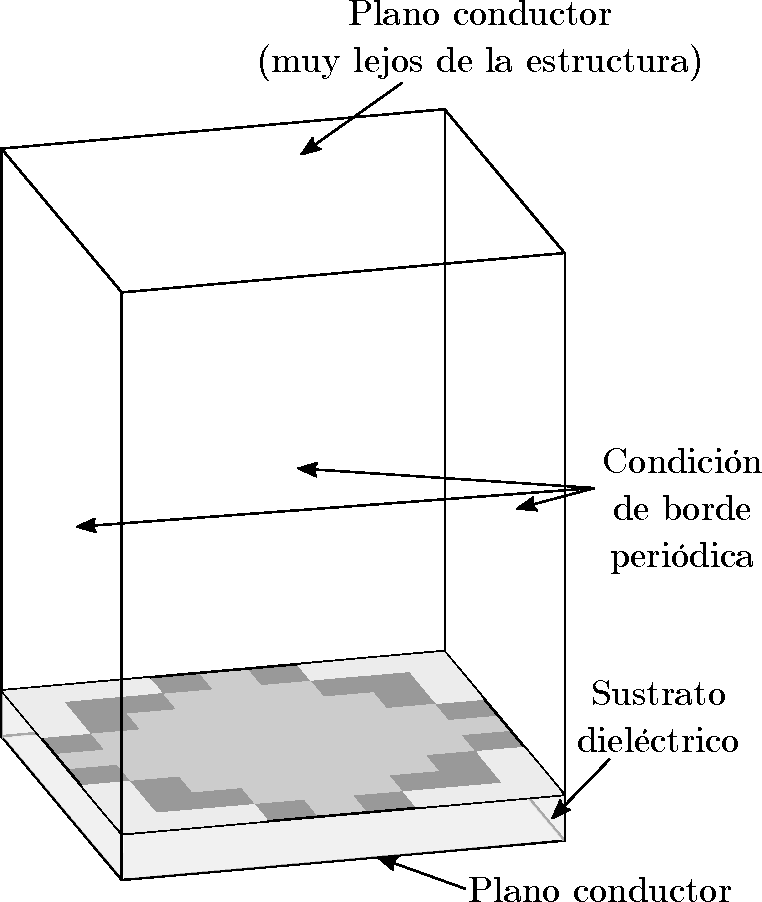
\includegraphics[width=0.6\textwidth]{Modelado/esquema-simulacion-periodica.pdf}
	\caption{Dominio de simulación de una celda unitaria de un metamaterial bidimensional, utilizando condiciones de borde periódicas.}
	\label{fig:esquema-simulacion-periodica}
\end{figure}

El uso de estas condiciones de borde periódicas deriva del teorema de Bloch-Floquet, tratado en la sección \ref{sec:bloch-floquet}. Como se muestra en la ecuación \ref{eq:comportamiento-periodico-campo-bloch}, el campo eléctrico (o magnético) resulta periódico, con la misma periodicidad que el material, a excepción de una variación de fase, dada por el valor de la constante de propagación $\beta$ del medio.

Para obtener el diagrama de dispersión, cada frecuencia $\omega$ debe estar asociada a una o más constantes de propagación de onda $\beta$. O, dicho de otra forma, dada una constante de propagación $\beta$, es necesario encontrar las autofrecuencias asociadas. Fijar el valor de la constante de propagación $\beta$, según la ecuación \ref{eq:comportamiento-periodico-campo-bloch}, equivale a establecer la diferencia de fase entre las paredes opuestas de la celda unitaria ($e^{-j\beta d}$). Una simulación del comportamiento en el tiempo, y una posterior transformada de Fourier para obtener el comportamiento en frecuencia, permite observar picos de amplitud de campo para algunas frecuencias en particular, que son las que autofrecuencias del problema. Dado que la misma diferencia de fase se puede obtener para frecuencias mayores (un ciclo más tarde), se presentará más de un modo.

Como se observó en la sección \ref{sec:diag-de-dispersion}, para la descripción del comportamiento de la relación de dispersión sólo es necesario el cálculo en la denominada zona irreducible de Brillouin, dado que a partir de reflexiones y transposiciones de la misma es posible reconstruir la celda unitaria en el espacio recíproco. Para el caso de celdas unitarias en que hay simetría sobre los ejes $x$ e $y$, y además hay simetría diagonal, la zona irreducible es un triángulo, como se mostró en la figura \ref{fig:rectangulo-cuadrado}.

De esta forma, únicamente hay que fijar, como condiciones de borde, diferencias de fase que se correspondan, entre los distintos puntos que forman una celda de Wignet-Seitz y que se corresponden a la zona irreducible de Brillouin.

% Fullwave: Baccarelli, Paulotto, impreso.
% Hacer estudio gráfico similar al CALOZ, pag 176.


\section{Análisis de campos y modos para distintas estructuras}
\label{sec_estructuras_propuestas}

\subsection{Metamaterial formado por parches cuadrados unidos por finas trazas \textit{microstrip}}
\label{sec:celdas-orlandi}

Uno de los metamateriales más fáciles de construir, y que en general presenta buenos resultados al mismo tiempo que mantiene una geometría sencilla es el que se observa en la figura \ref{fig:celda-orlandi}. En la misma, $d$ es el lado de la celda unitaria (cuadrada), $l$ es el tamaño del lado del cuadrado metálico (de cobre), y $l_m$ y $w_m$ son el largo y el ancho de los puentes que comunican a los parches, respectivamente.

\begin{figure}[h]
	\centering
	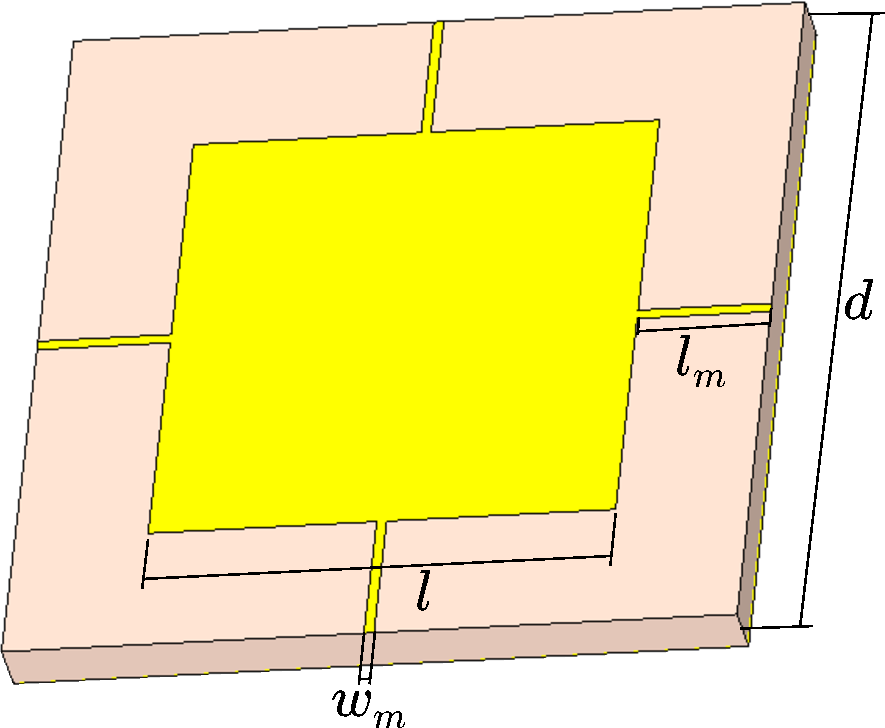
\includegraphics[width=0.4\textwidth]{Modelado/orlandi-celda.pdf}
	\caption{Celda unitaria de un metamaterial formado por parches cuadrados unidos por finas trazas \textit{microstrip}.}
	\label{fig:celda-orlandi}
\end{figure}

Esta geometría resulta sencilla de analizar, debido principalmente a que, como se estudió en la sección \ref{sec:modelo_analitico}, cada aspecto de la misma tiene un equivalente circuital, al menos para las frecuencias más bajas, que varía en función de los parámetros constructivos. La celda unidad propuesta posee una simetría tal que permite realizar un análisis en una zona de Brillouin triangular, como la que se mostró, teóricamente, en la figura \ref{fig:explicacion-zona-brillouin}.

Aplicando el análisis de autovalores explicado en la sección precedente, es posible obtener, para cada condición de borde periódica en que va variando la fase de las paredes opuestas que conforman el contorno condicionado, un conjunto de frecuencias que representan los modos de propagación en cada dirección analizada, lo que permite crear un diagrama de dispersión, similar al mostrado en la figura \ref{fig:diagrama-dispersion-vacio-2d}, aunque con modos superiores.

\begin{figure}[h]
	\centering
	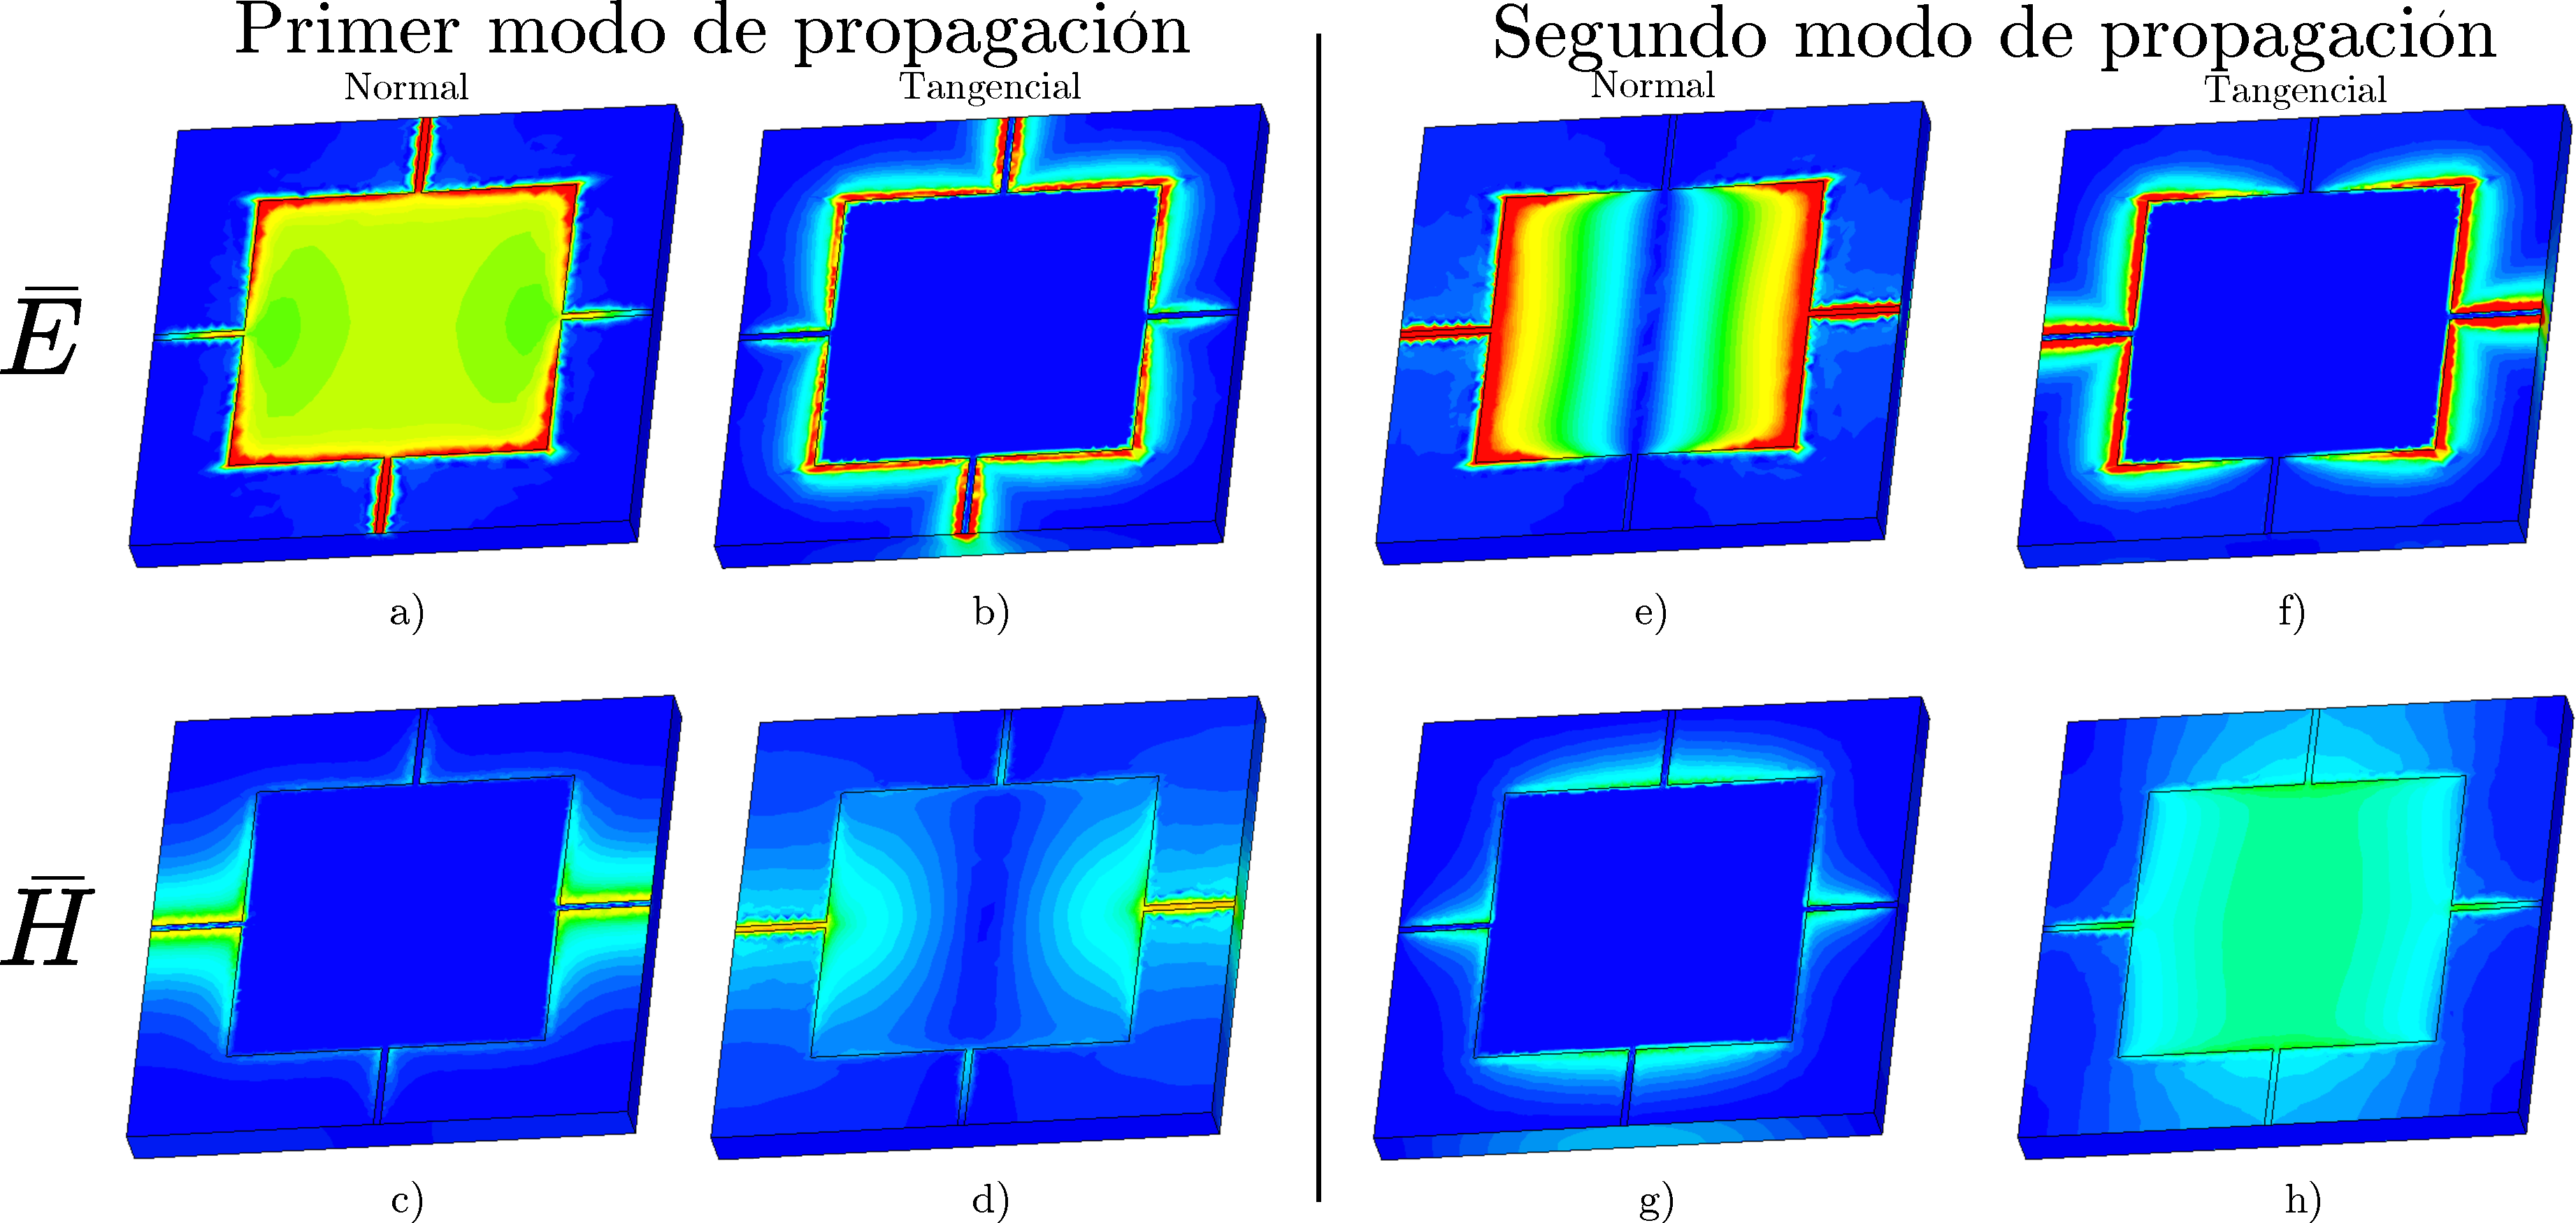
\includegraphics[width=1\textwidth]{Modelado/orlandi-modo1-Enorma-Etangencial.pdf}
	\caption{Comportamiento, en promedio temporal, de los campos eléctrico y magnético sobre una celda unitaria formada por un parche central y 4 puentes laterales, para el primer y segundo modo de propagación.}
	\label{fig:orlandi-analisis-campos}
\end{figure}

En la figura \ref{fig:orlandi-analisis-campos} se ilustran\footnote{Debido a la naturaleza de la simuación con autovalores, que no impone una tensión inicial, los valores obtenidos de los campos no son representativos de la situación física (aunque sí la morfología espacial). Estos valores obtenidos, no mostrados en la figura, suelen ser altos debido al mecanismo de simulación. El análisis que se pretende realizar aquí del comportamiento de los campos es puramente conceptual.}, para los dos primeros modos de propagación, los campos eléctrico y magnético en dirección normal y tangencial a la superficie, considerando una dirección de propagación horizontal (equivalente al punto $M$ en la figura \ref{fig:explicacion-zona-brillouin}).

En la figura \ref{fig:orlandi-analisis-campos} a) se muestra el comportamiento del campo eléctrico promedio perpendicular a la superficie para el primer modo de propagación. Resulta claro que el mismo se concentra debajo del parche metálico que conforma a la celda unitaria, debido a que la presencia de un plano de tierra genera un comportamiento de planas planas paralelas, conformando efectivamente un capacitor. Es también notoria la presencia de campo eléctrico en dirección normal a la superficie en los puentes \textit{microstrip} superior e inferior, debido principalmente a que no hay movimiento de cargas en dirección longitudinal a los mismos, sino que actúan como extensiones al parche central, aumentando ligeramente la capacidad del dispositivo.

El campo eléctrico en la dirección tangencial, también para el primer modo de propagación, es ilustrado en la figura \ref{fig:orlandi-analisis-campos} b), y permite observar la existencia de notorios efectos de \textit{fringing} alrededor de todo el parche, que deben ser considerados en el análisis. Estos efectos son mayores sobre los puentes superior e inferior, nuevamente, mientras que sobre los puentes ubicados horizontalmente parece no haber concentración de cargas. Esto se confirma al analizar las figuras \ref{fig:orlandi-analisis-campos} c) y d), que ilustran el campo magnético en dirección normal y tangencial a la superficie, respectivamente. Se puede observar que no existen campos magnéticos normales a la superficie debajo del parche metálico, sino que, como muestra la figura d), son puramente tangenciales. Debajo del parche, entonces, para el primer modo de propagación, los campos son cuasi-TEM. La presencia de campo magnético sobre los puentes horizontales corrobora la hipótesis de que sobre los mismos se genera corriente, que ingresa al parche metálico para ser conducida.

\begin{figure}[h]
	\centering
	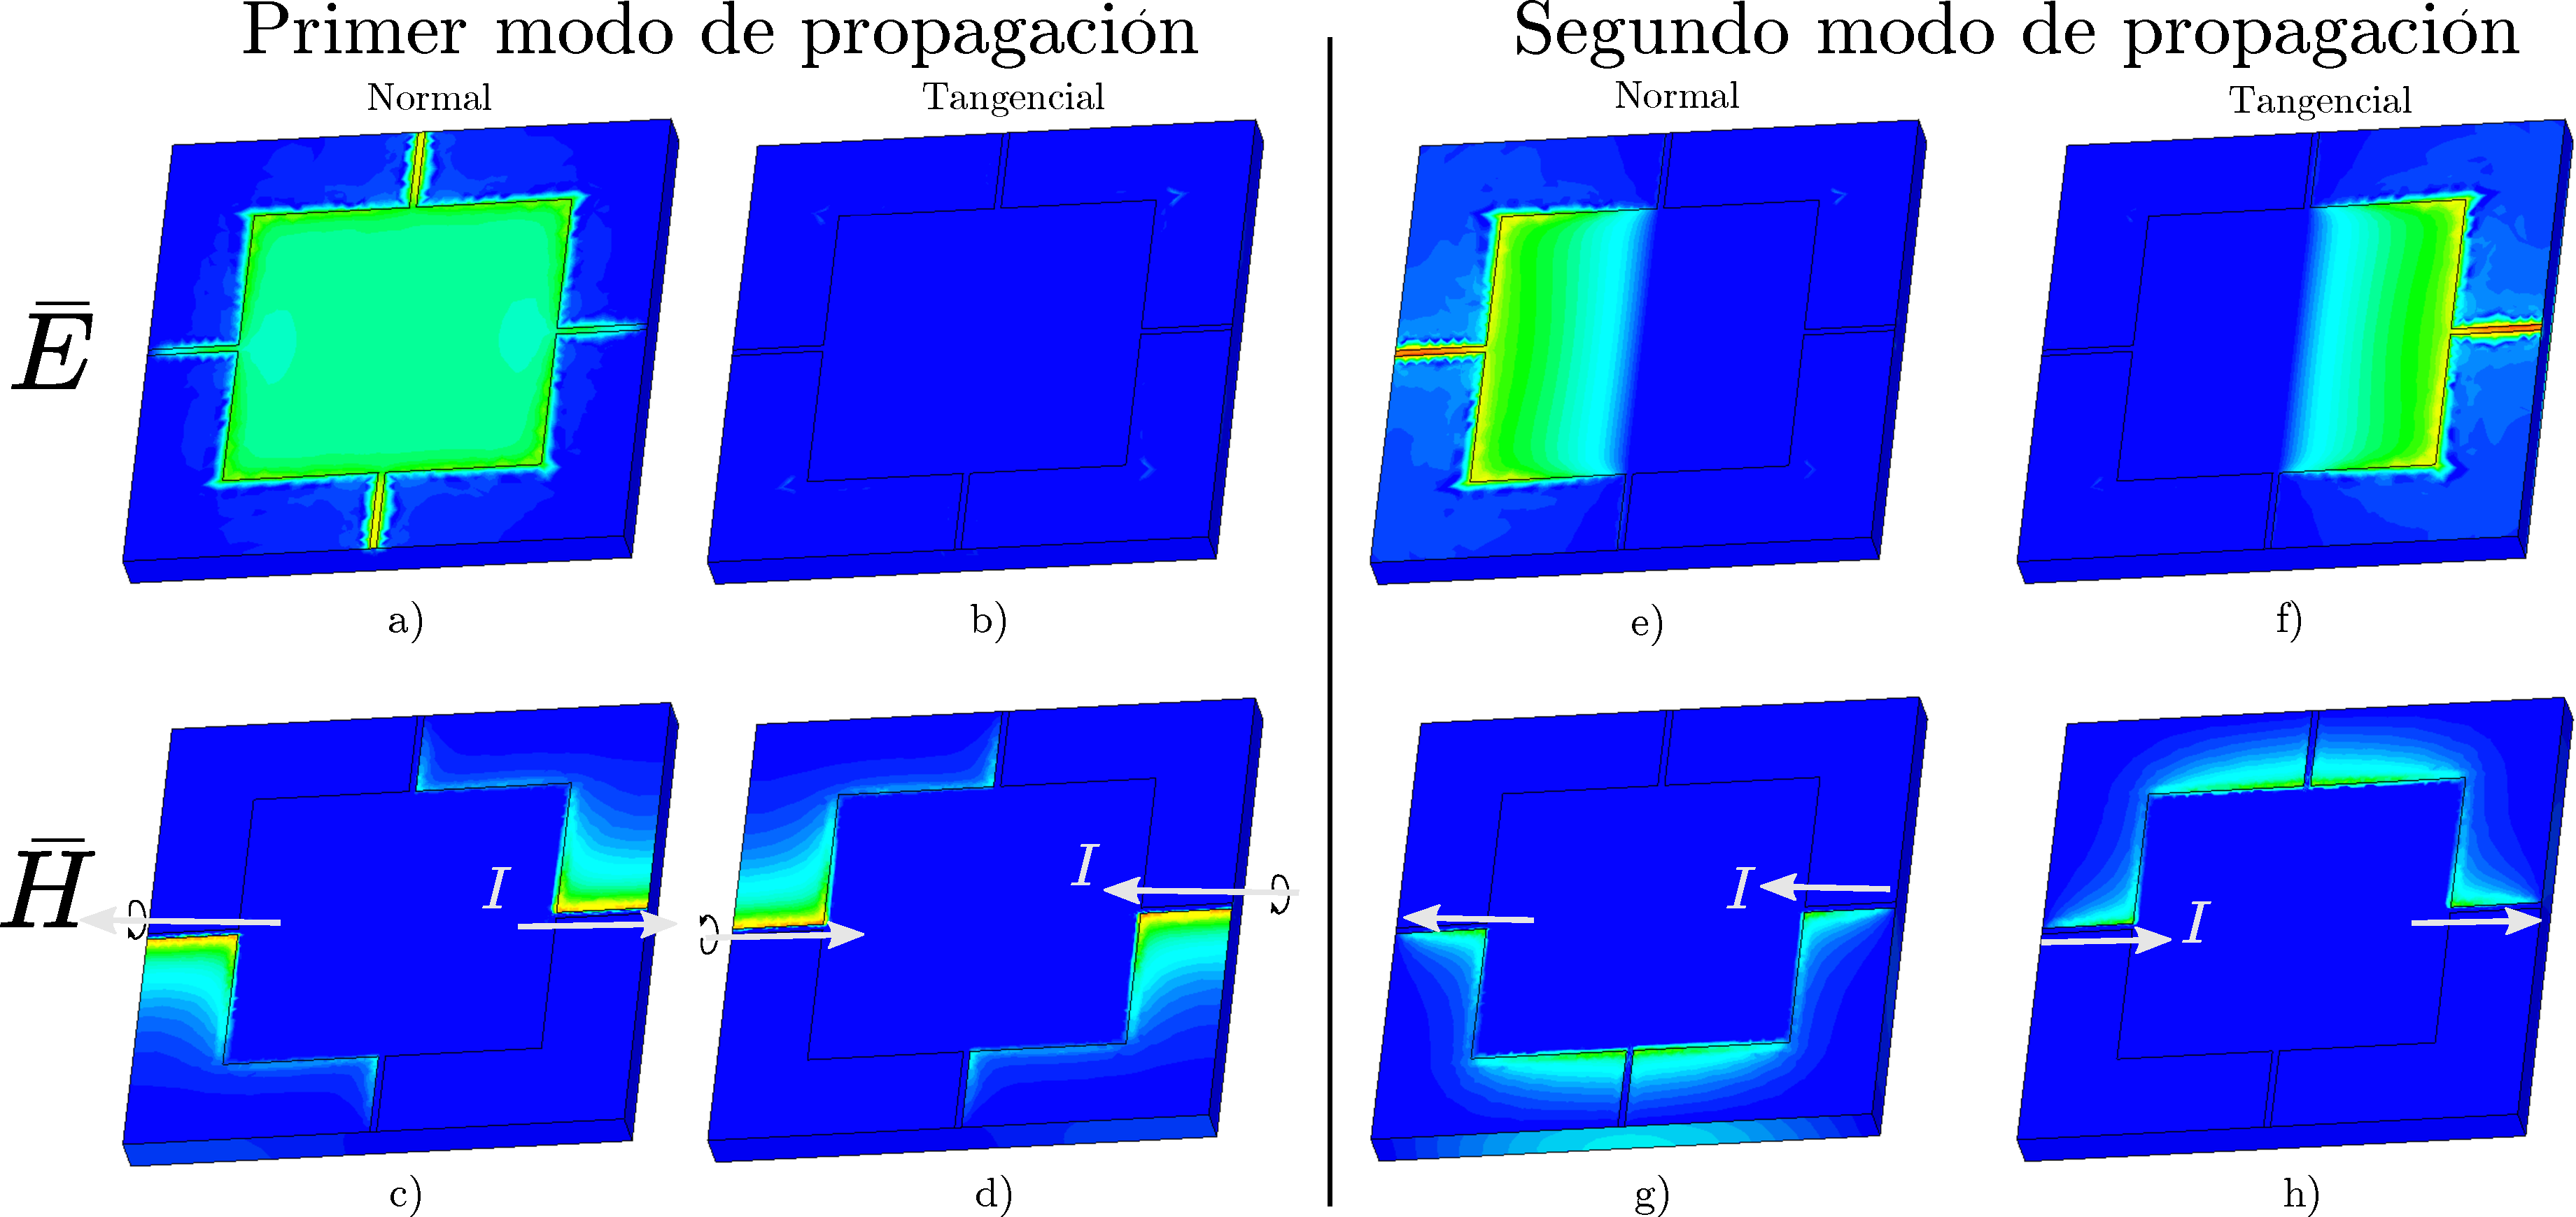
\includegraphics[width=1\textwidth]{Modelado/orlandi-modo1-EH-fases.pdf}
	\caption{Comportamiento, para dos tiempos diferentes, de los campos eléctrico y magnético normales a la superficie, sobre una celda unitaria formada por un parche central y 4 puentes laterales, para el primer y segundo modo de propagación.}
	\label{fig:orlandi-analisis-campos-fases}
\end{figure}

El análisis para el primer modo de propagación continúa en la figura \ref{fig:orlandi-analisis-campos-fases}. En las figuras \ref{fig:orlandi-analisis-campos-fases} a) y b) se muestra el comportamiento del campo eléctrico para dos momentos de tiempo diferentes. Se observa que el parche almacena cargas durante un breve tiempo, y las expele inmediatamente después. Esto se ve corroborado por el comportamiento del campo magnético normal a la superficie, mostrado en escala lineal en las figuras \ref{fig:orlandi-analisis-campos-fases} c) y d), para dos tiempos distintos, y donde se ven colores cuando el campo es positivo en la dirección perpendicular saliente a la superficie del parche. A través del uso de la regla de la mano derecha, se pueden deducir las direcciones de las corrientes sobre los puentes, que son las especificadas por flechas, y donde se observa que son opuestas en el primer modo. Es decir, de forma intuitiva, las corrientes son entrantes al parche de todas direcciones al mismo tiempo, y son salientes del mismo hacia todas direcciones en un tiempo subsiguiente. De esta forma, el parche posee cargas positivas completamente en un tiempo, y luego cargas negativas en el tiempo siguiente, lo cual coincide con la intuición del concepto de un primer modo de propagación, y con el análisis intuitivo detallado.

El segundo modo de propagación, para la misma dirección y posición sobre el diagrama de dispersión (punto "M"), posee un comportamiento más complejo. Como se observa en la figura \ref{fig:orlandi-analisis-campos} e), el campo eléctrico presenta un cero en el centro de la celda unidad, en la figura f) es coherente con esta observación, dado que cerca del centro y de los puentes verticales no hay campo de \textit{fringing}. El campo magnético, por otro lado, mostrado en las figuras g) y h), nuevamente no parece permitir concebir corrientes sobre los puentes verticales, aunque sí en el interior del parche metálico propiamente dicho.

El análisis de dos tiempos diferentes dentro del ciclo para el segundo modo de propagación, mostrado en las figuras \ref{fig:orlandi-analisis-campos-fases} e)-h), permite comprender más intuitivamente el comportamiento. Se observa que el parche central es excitado (posee campo eléctrico vertical) en dos tiempos diferentes, y sólo una de sus mitades lo es cada vez. Hay un desfasaje de $180^\circ$ entre ambos lados del parche. Observando el campo magnético, resula también intuitivo considerar que cuando la mitad izquierda del parche está excitada, es decir, cuando posee cargas almacenadas, formando un capacitor con el plano de tierra, se genera una corriente hacia la celda vecina, que posee un parche con tensión opuesta. En el lado derecho, el efecto es análogo. Es importante notar que, al contrario que en el caso del primer modo, en el segundo modo de propagación las corrientes de los puentes tienen el mismo sentido en cada tiempo.

La figura \ref{fig:dibujito-modos} ilustra, de forma esquemática e informal, el comportamiento de la fase del campo eléctrico para ambos modos de propagación, de manera que se pueda apreciar el requerido aumento de frecuencia para la concreción del segundo modo.

\begin{figure}[h]
	\centering
	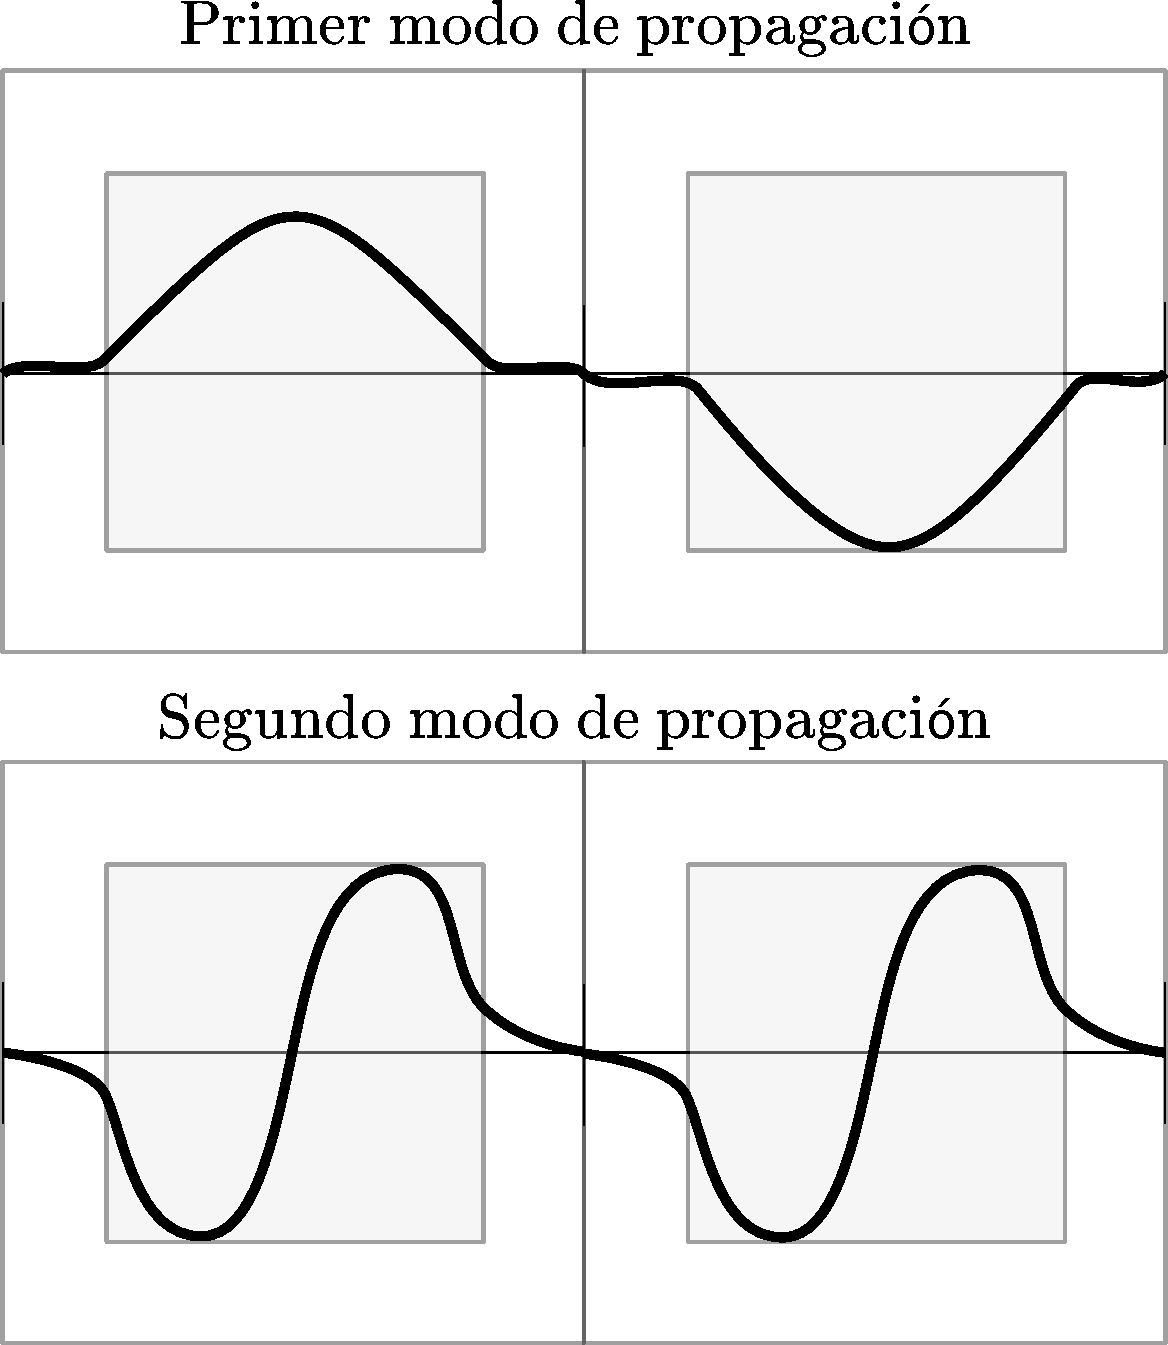
\includegraphics[width=0.4\textwidth]{Modelado/modos-de-propagacion-ilustracion.pdf}
	\caption{Comportamiento, para dos tiempos diferentes, del campo eléctrico sobre una celda unitaria formada por un parche central y 4 puentes laterales, para el primer y segundo modo de propagación.}
	\label{fig:dibujito-modos}
\end{figure}


Para comprender el efecto de la variación de distintos parámetros geométricos, se realizaron varias simulaciones, obteniendo de ellas los diagramas de dispersión.

\subsubsection{Análisis de un diagrama de dispersión típico}

En la figura \ref{fig:diag-dispersion-tipico} se puede observar un diagrama de dispersión típico.

\begin{figure}[h]
	\centering
	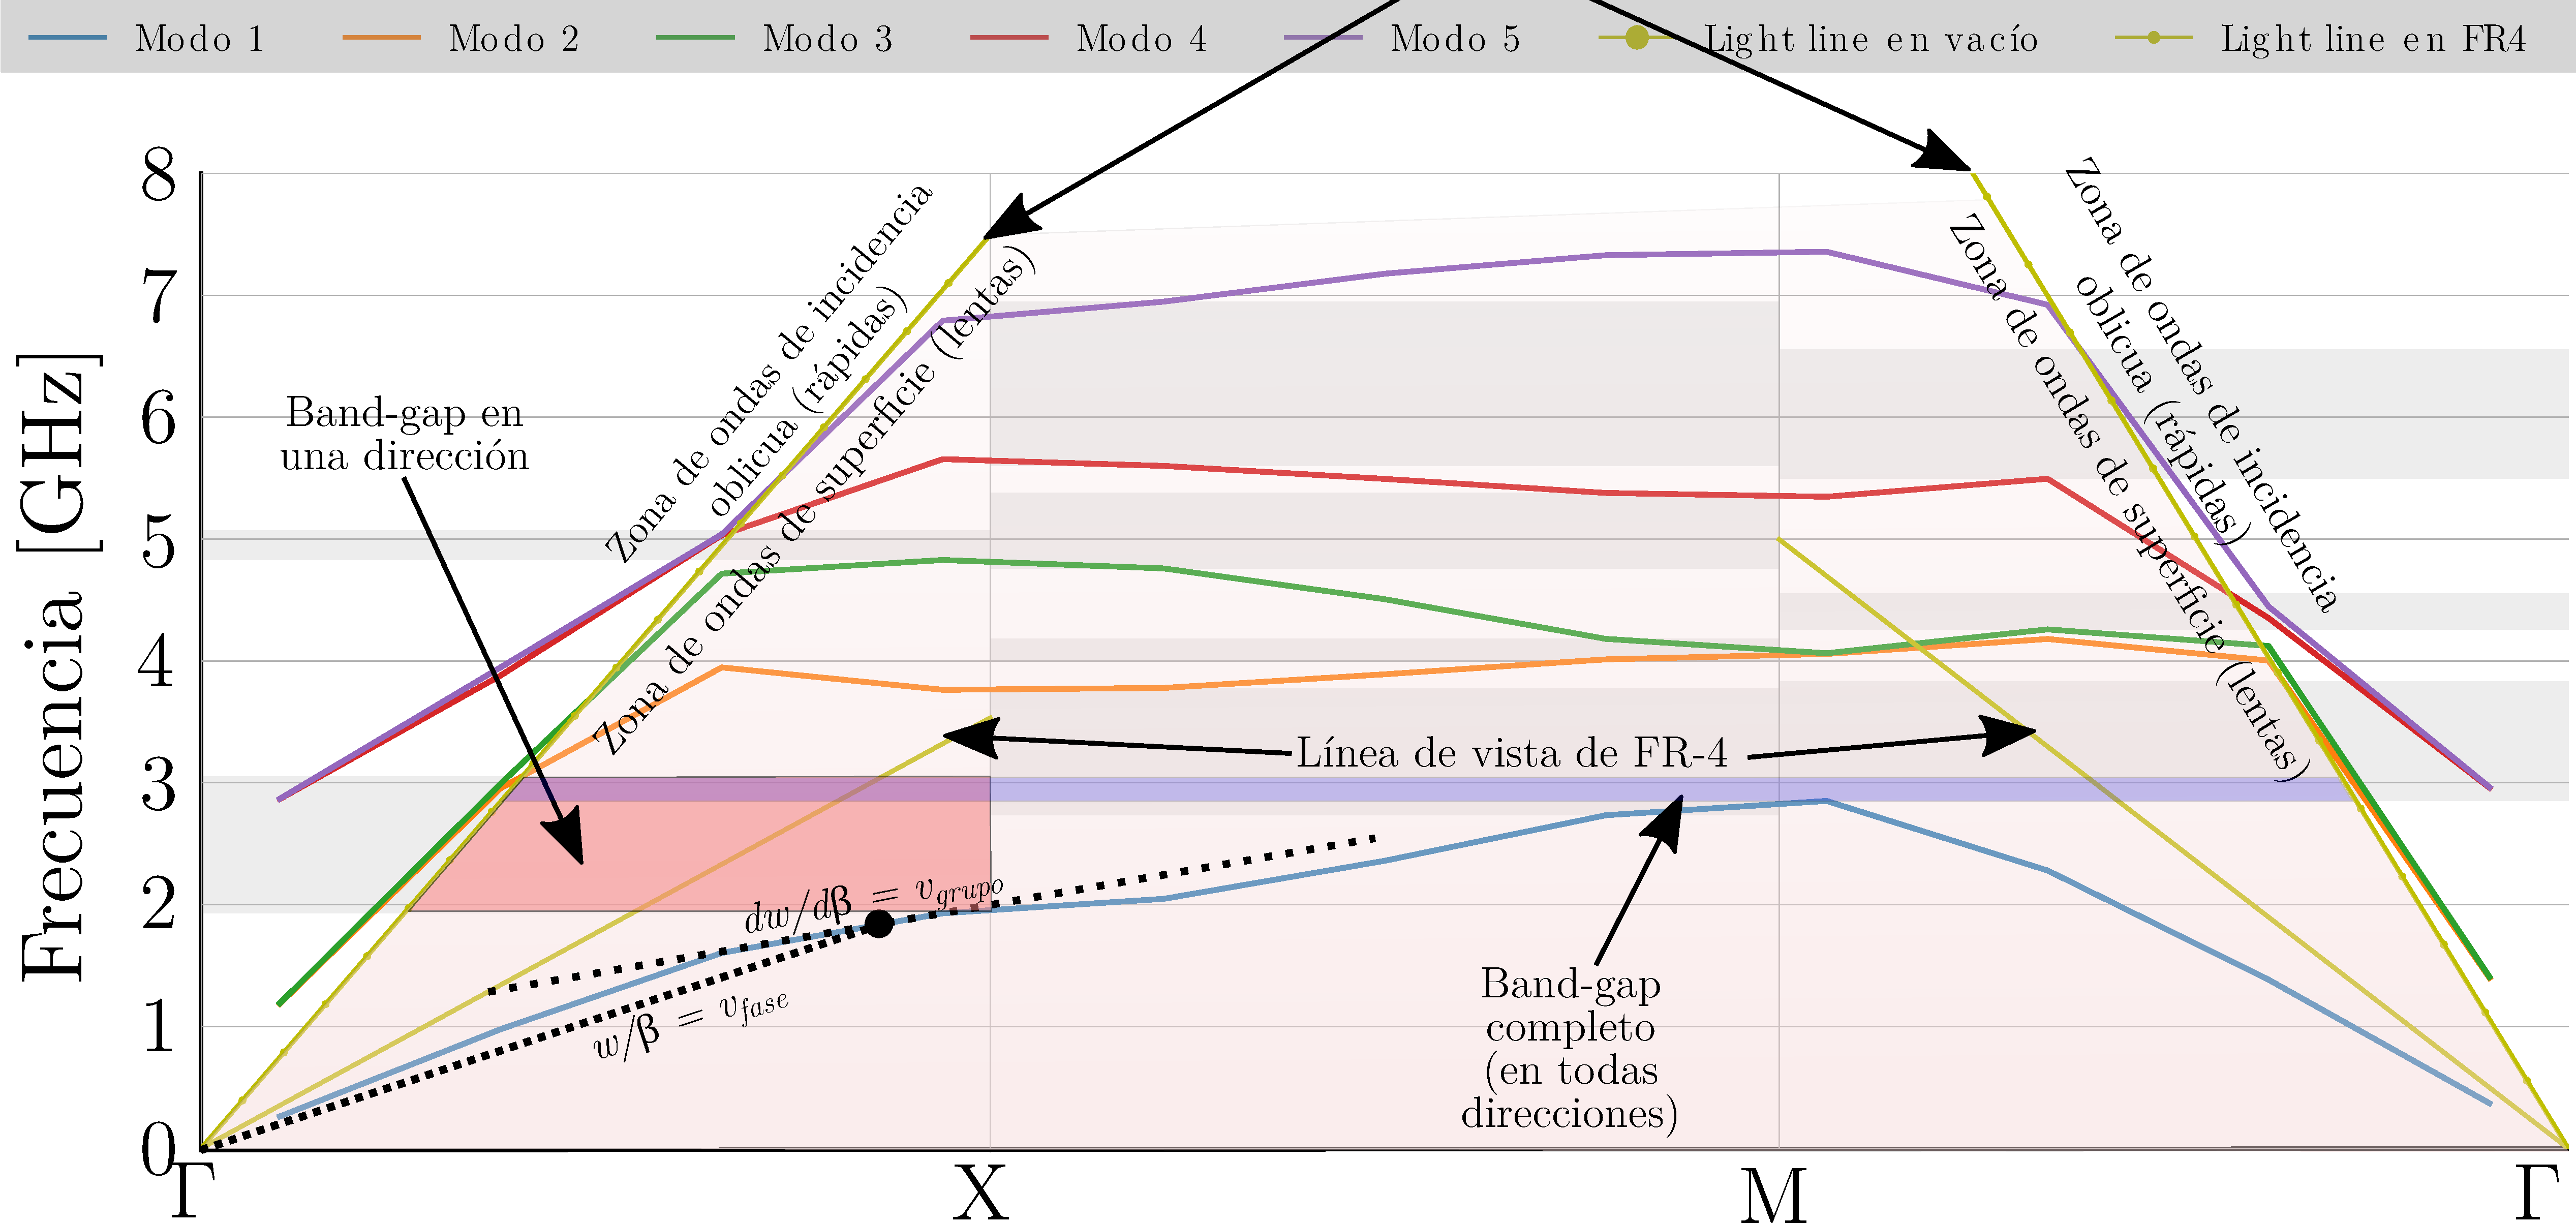
\includegraphics[width=\textwidth]{Modelado/ejemplo-diag-disp.pdf}
	\caption{Ejemplo típico de un diagrama de dispersión que presenta un metamaterial bidimensional.}
	\label{fig:diag-dispersion-tipico}
\end{figure}

La línea azul corresponde al primer modo de propagación, la marrón al segundo, la verde al tercero, la roja al cuarto y la violeta al quinto. Además, se dibujaron las líneas de vista (\textit{light-lines}) para vacío y para FR-4, que indican el comportamiento de una onda plana que circula por esos materiales. Representan el corte del diagrama de dispersión tridimensional mostrado en la figura \ref{fig:diagrama-dispersion-vacio-3d} sobre los bordes de la celda de Brillouin, como se ve en la figura \ref{fig:diagrama-dispersion-vacio-2d}, para los dos materiales. La línea de vista del FR-4 presenta, naturalmente, una pendiente menor a la del vacío, pues la velocidad de propagación sobre ese medio es menor.

La línea de vista del vacío separa las llamadas ondas lentas (\textit{slow waves}), que poseen una velocidad de fase menor a la del vacío ($c$), de las ondas rápidas (\textit{fast waves}), con velocidad de fase superior a $c$. Dado que, para el vacío, $\beta=\omega/c$, si se extiende a definición a dos dimensiones, se obtiene que $\beta_x^2 + \beta_y^2 = \omega^2/c^2$. Cuando el valor de $|\beta|$ supera al correspondiente a la propagación en el vacío para la misma frecuencia, necesariamente la velocidad de fase es menor ($\beta = \omega / v_p$). Cuando la velocidad es mayor, es decir, cuando se analizan resultados para pares $(\omega,\beta)$ que están por encima de la línea de vista, el estudio no se da sobre ondas de superficie, sino sobre ondas incidentes o reflejadas con ángulo determinado. En algunos casos \cite{Maci:Pole-zero-matching}, para algunos usos de metamateriales (especialmente cuando se los diseña de forma que actúen como paredes conductoras magnéticas), esa zona del diagrama de dispersión resulta de gran utilidad \cite{Yang:EBGAntennas}.

Las zonas demarcadas en gris representan, para cada una de las direcciones analizadas, la zona de frecuencias prohibidas o \textit{band-gap}. En particular, para la zona $\Gamma-X$, el primer \textit{band-gap} se demarcó en rojo. Se debe tener en cuenta que se calculan los \textit{band-gaps} para  las tres direcciones de forma separada. Existe un \textit{band-gap} completo (en azul), cuando existe en todas las direcciones analizadas. Para las frecuencias dentro de la zona prohibida completa, no existirá ángulo de incidencia que permita su propagación. Es importante notar que, para los intervalos $\Gamma-X$ y $M-\Gamma$, las zonas prohibidas para la propagación de ondas lentas (\textit{slow-waves}) de superficie se calculan por debajo de la línea de vista del vacío. Por encima de dicha línea, las ondas se propagan libremente.

En general, el diseño de EBGs tiene como objetivo aumentar el ancho de la banda prohibida de frecuencias para la propagación de ondas de superficie, la variación de la frecuencia central de los \textit{band-gaps}, y la independización del mismo de la dirección de propagación (que equivale a lograr \textit{band-gaps} completos). Estos objetivos se logran modificando la geometría de la celda unitaria, aumentando el acoplamiento entre las mismas y conectando los parches al plano de tierra \cite{Marcela:Tesis}. La independización de las zonas prohibidas para cualquier dirección azimutal de propagación de ondas de superficie requiere celdas simétricas, aunque para ciertas aplicaciones la anisotropía es buscada \cite{Maci:Pole-zero-matching}.

El diagrama de dispersión, además, da una idea de las velocidades de fase ($v_p = w/\beta$) y grupo ($v_g = d\omega / d\beta$) para los modos existentes.

%% Analizar Vfase, Vg, y por qué cambian según la posición en el diagrama de briloouin. Ver Mohajer-Irarani, Ramahi. Esto va de la mano con ¿por qué los ebgs son tanto más chico que lambda? porque la velocidad de propagación es menor adentr del sustrato, en los modos atrapadao. Eso se puede ver en Goussetis, Feresidis, Vardaxoglow (periodically loaded 1 D metallodielectric..). Vincular con el tema de Forward y Backward waves (Kubacki, Lamari, Rudyk).

%% Se debe tener en cuenta que un bandgap no indica que no hay transferencia de poencia. Puede hacer un bandgap, que significa que no hay ondas propagantes, pero sí existen ondas evanescentes, que pueden, si llegan con suficiente energía, excitar a celdas cercanas y generar leaky waves y transporte de potencia. Es un gran problema. Ver Mohajer-Irarani, Ramahi.

%%%% ESTARRIA MUY BUENO EN ALGUN MOMENTO PONER UN DIAGRAMA DE DISPERSION DE UN SLAB DESNUDO Y OTRO DE UN SLAB CON DIELECTRICO; PARA UNIIR CON LA PARTE TEÓRICA ANTERIOR.

\subsubsection{Efecto de la variación del ancho del puente \textit{microstrip}}

La primera variación analizada es la del ancho de los puentes \textit{microstrip} que unen a los parches metálicos que conforman la estructura. Estableciendo una celda de $2\;\text{cm}$ de lado, y un parche de $1.8\;\text{cm}$, para el caso de sustrato FR4 de $1.6\;\text{mm}$ de espesor, se obtuvieron los diagramas de dispersión sobre el borde de la celda de Brillouin que se muestran en la figura \ref{fig:diagdisp-orlandi-variacion-ancho-puente}.

\begin{figure}[h]
	\centering
	\includegraphics[width=1\textwidth]{Modelado/Orlandi-DeltaAnchoConector.pdf}
	\caption{Diagramas de dispersión para la variación del ancho de los puentes \textit{microstrip} que conforman una celda unitaria cuadrada, de lado $2\;\text{cm}$, parche de $1.8\;\text{cm}$, con sustrato de FR-4 de $1.6\;\text{mm}$ de espesor.}
	\label{fig:diagdisp-orlandi-variacion-ancho-puente}
\end{figure}

En la misma se observa que la formación de una zona prohibida completa entre los dos primeros modos de propagación, se ve dificultada cuando el ancho del puente aumenta, debido a que, para todas las direcciones de propagación, el ancho de los \textit{band-gaps} disminuye drásticamente.


\begin{figure}[h]
	\centering
	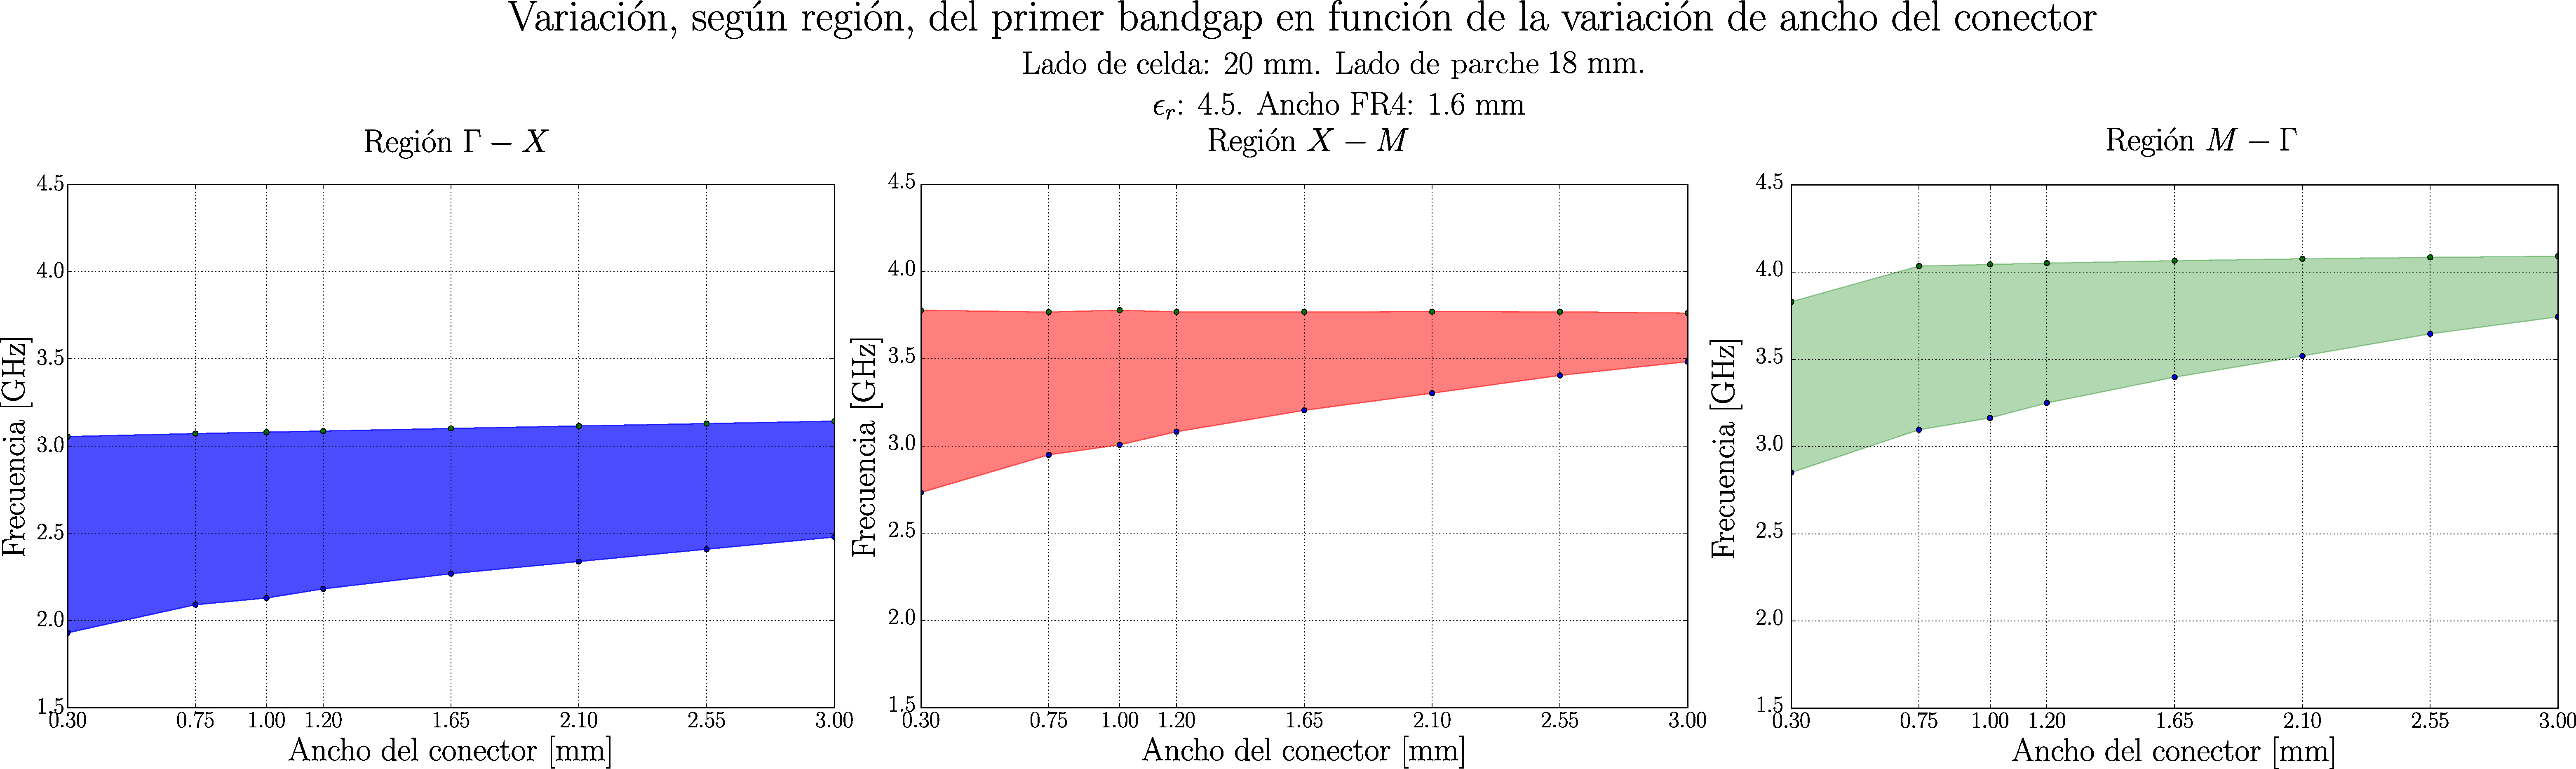
\includegraphics[width=1\textwidth]{Modelado/Orlandi-DeltaAnchoConector-comparacion.pdf}
	\caption{Comparación del ancho del primer band-gap (entre el primer y el segundo modo de propagación) para las tres direcciones analizadas, en función del ancho del puente que une los parches metálicos.}
	\label{fig:comparacion-diagdisp-orlandi-variacion-ancho-puente}
\end{figure}

La principal causa se puede deducir de la figura \ref{fig:comparacion-diagdisp-orlandi-variacion-ancho-puente}, donde es notorio el crecimiento generalizado de las frecuencias necesarias para obtener el primer modo de propagación (la curva azul de la figura \ref{fig:diagdisp-orlandi-variacion-ancho-puente} se eleva), lo que se condice con una aumento en la velocidad de propagación en el metamaterial. Una explicación intuitiva, válida únicamente para las frecuencias en que se puede aplicar el modelo cuasiestático y considerar corrientes y tensiones sobre los conductores que conforman la estructura, se basa en la posible disminución de la resistencia al paso de corriente, lo que permite una carga y descarga del capacitor de placas planas paralelas (formado por el parche y el plano de tierra) más rápida.

Para modos superiores, especialmente para el rango de frecuencias entre el cuarto y el quinto modo, existe una zona prohibida que se extiende en todas direcciones, pero se da para frecuencias mucho más altas, de escaso valor práctico.

\clearpage
\subsubsection{Efecto del escalamiento de la celda unitaria}

\begin{figure}[h]
	\centering
	\includegraphics[width=1\textwidth]{Modelado/Orlandi-DeltaTamanioCelda-RelacionParcheFija.pdf}
	\caption{Diagramas de dispersión para la variación del ancho de las celdas unitarias (y, en consecuencia, también del parche que contiene) que conforman una celda unitaria cuadrada. El lado del parche es $3/4$ del lado de la celda unitaria. El sustrato de FR-4 de $1.6\;\text{mm}$ de espesor.}
	\label{fig:diagdisp-orlandi-variacion-tam-celda-unitaria}
\end{figure}

\begin{figure}[h]
	\centering
	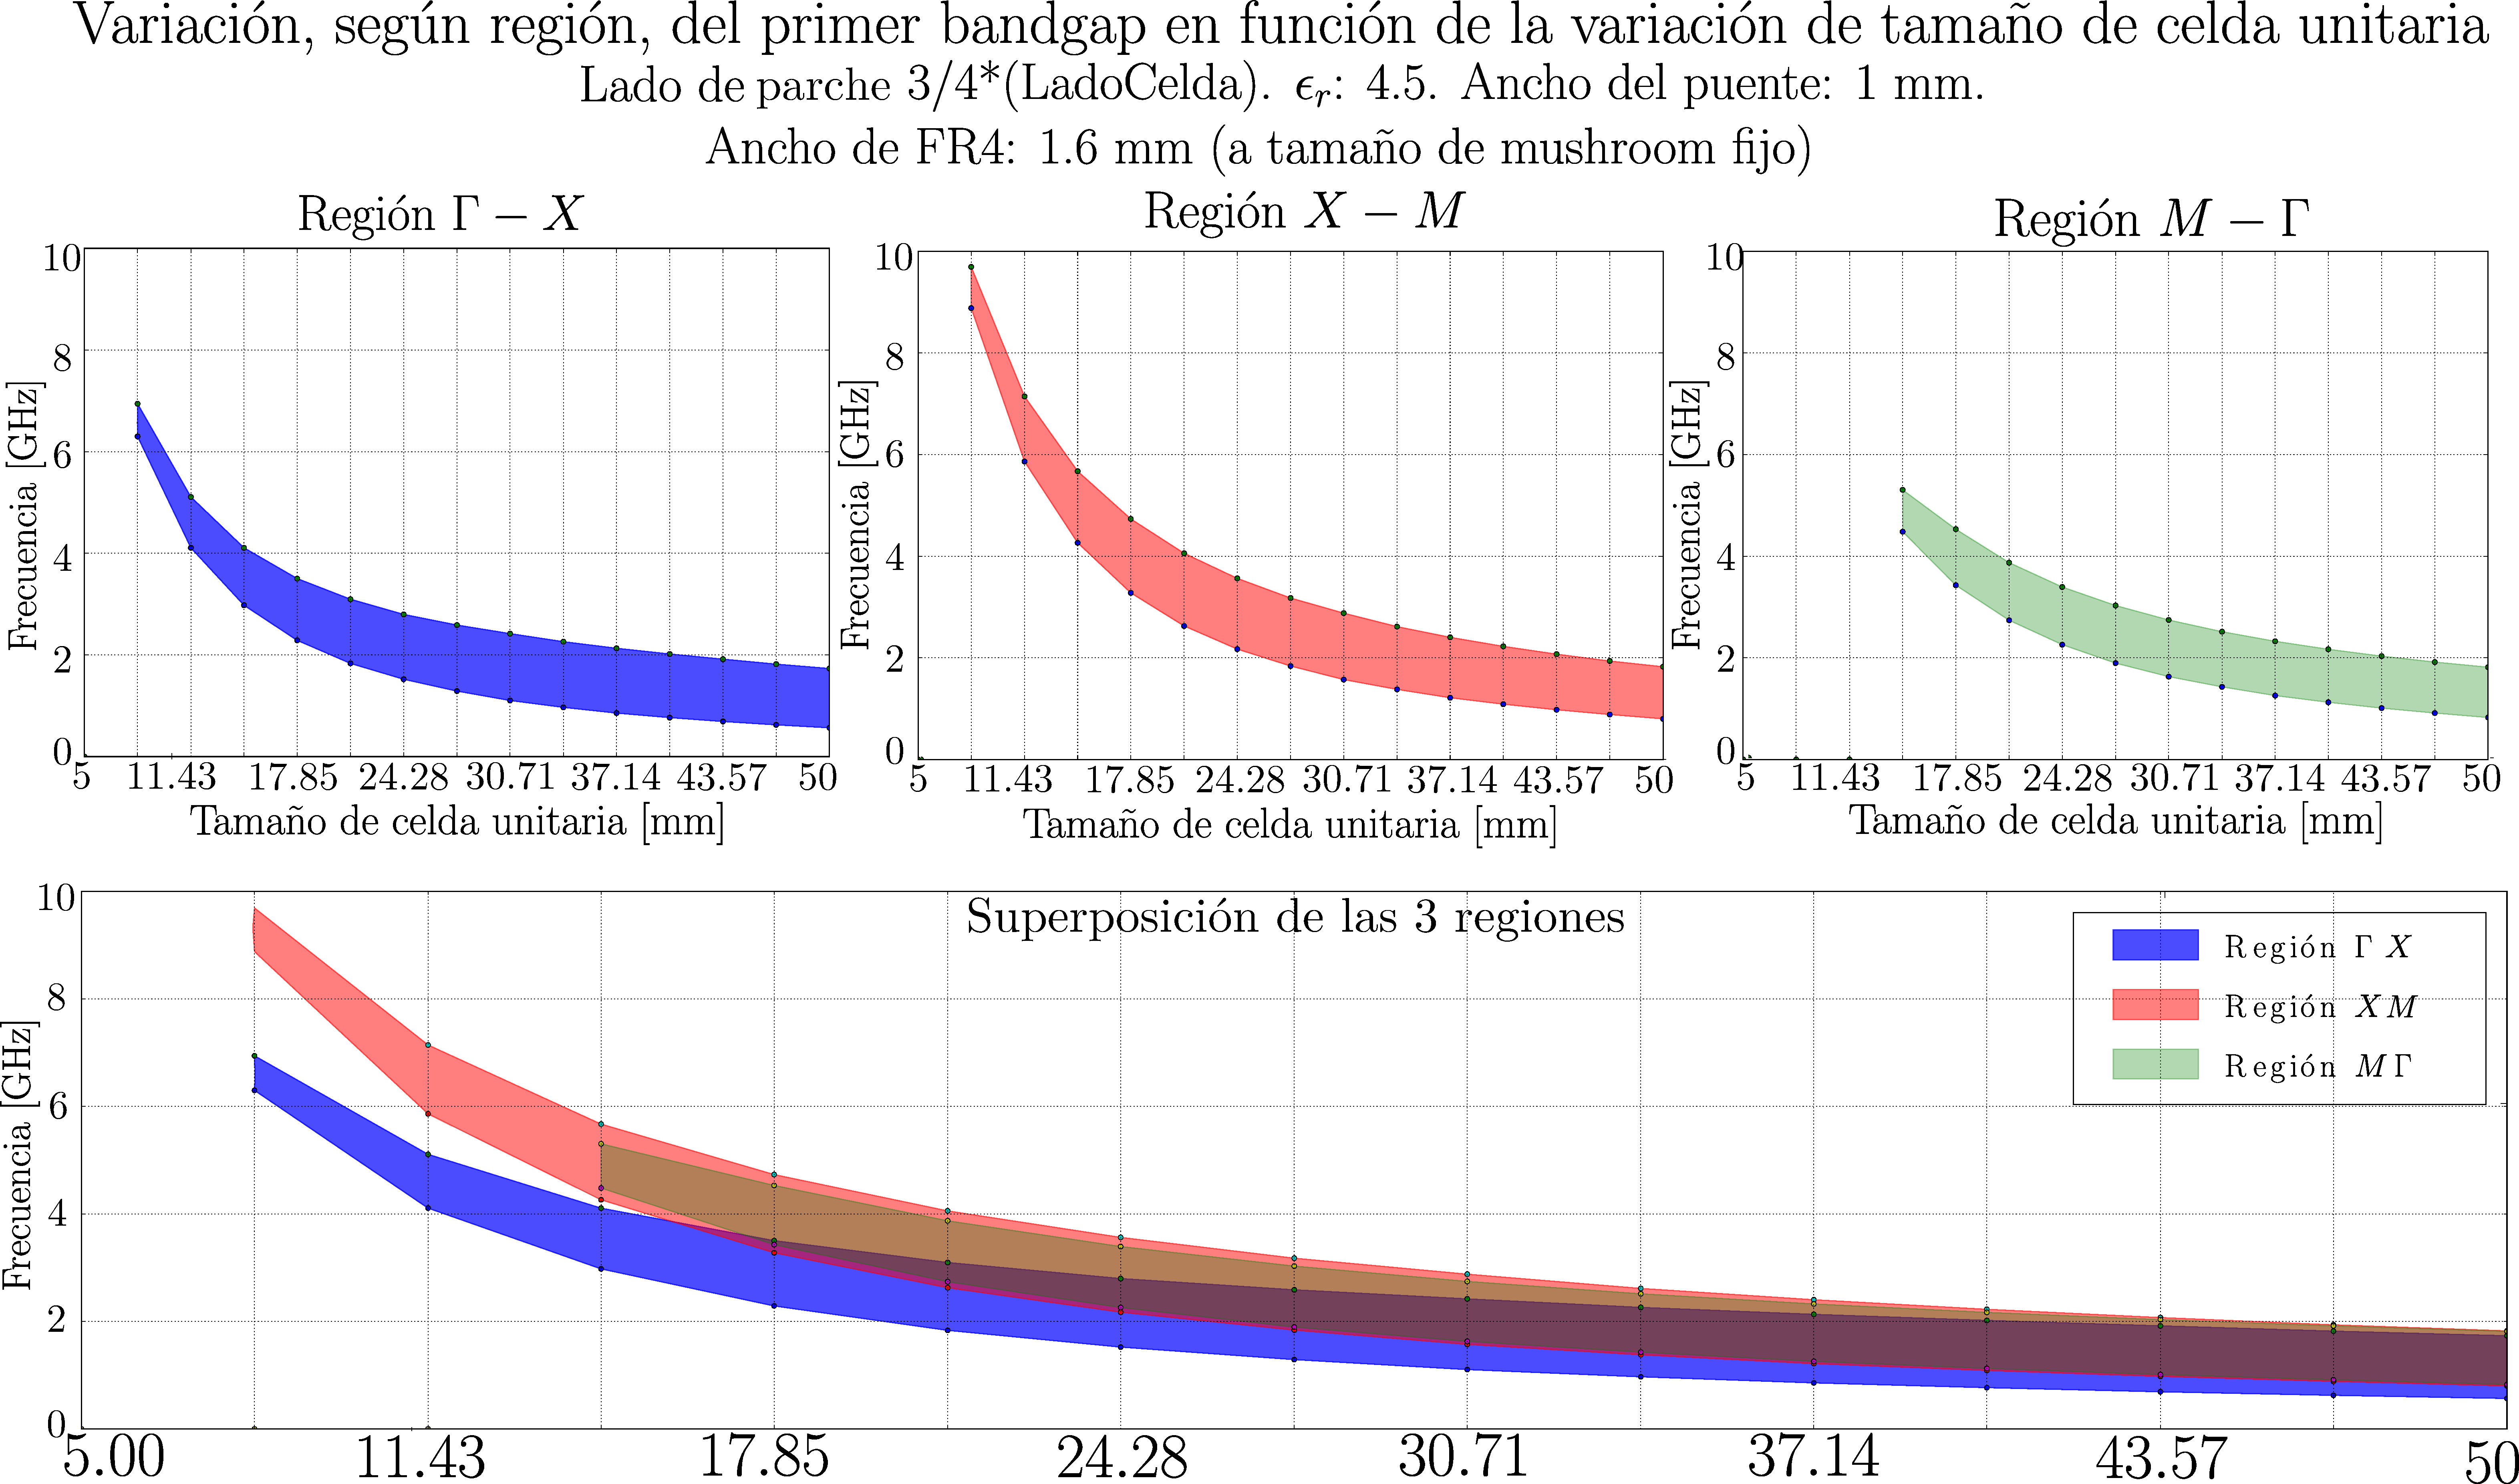
\includegraphics[width=1\textwidth]{Modelado/Orlandi-DeltaTamanioCelda-RelacionParcheFija-Comparacion.pdf}
	\caption{Compraración del ancho del primer band-gap (entre el primer y el segundo modo de propagación) para las tres direcciones analizadas, en función del tamaño de la celda unitaria.}
	\label{fig:comparacion-diagdisp-orlandi-variacion-tam-celda-unitaria}
\end{figure}

Un escalamiento de la celda unitaria, debido a la linealidad de las ecuaciones de Maxwell, debería únicamente generar un cambio en las frecuencias centrales de los \textit{band-gaps}. Para celdas unitarias pequeñas, las frecuencias centrales de las zonas prohibidas son altas, y resulta más difícil obtener un \textit{bandgap} completo, como se observa en la figura \ref{fig:diagdisp-orlandi-variacion-tam-celda-unitaria}.

En la figura \ref{fig:comparacion-diagdisp-orlandi-variacion-tam-celda-unitaria} se puede observar el comportamiento del primer \textit{bandgap} (ubicado entre el primer y el segundo modo de propagación), en función del tamaño de la celda unitaria analizada. A medida que la misma disminuye, las frecuencias centrales decaen a un ritmo de $sarasa$. La variación del tamaño de la celda unitaria, por sí solo, facilita la superposición de zonas prohibidas en todas las direcciones sólo para frecuencias bajas, y cuando la celda unitaria es grande. La superposición de las tres direcciones de propagación analizadas se puede observar en la gráfica inferior de la figura \ref{fig:comparacion-diagdisp-orlandi-variacion-tam-celda-unitaria}.

El comportamiento de la primer zona prohibida se puede explicar intuitivamente considerando que, de no variar la velocidad de propagación en el medio, y dado que $\omega =k*v_p$, entonces al variar el número de onda requerido por aumentar el tamaño de la celda unitaria (disminuye, permitiendo que el primer modo se corresponda con una longitud de onda mayor), el valor de $\omega$ debe disminuir en consecuencia.

A este efecto se debe añadir el correspondiente al aumento del efecto capacitivo por el aumento del tamaño del parche. Si se considera, como se explicó antes, que un análisis a bajas frecuencias, utilizando razonamientos cuasiestáticos, nos conduce a un filtro LC equivalente. La frecuencia de resonancia de ese tipo de filtro es, en general, y sin considerar pérdidas, $f_r \approx 1/\sqrt{LC}$. Dado que se está escalonando la celda unitaria, y que por tanto también está creciendo el tamaño del parche, el valor de la capacidad aumenta. La relación entre la capacidad y el tamaño del parche es cuadrática, como se puede ver en la ecuación \ref{eq:Cp_Lp}, y la inductancia no aumentará apreciablemente en comparación. De esta forma: $f_r \propto 1/\sqrt{l^2} = 1/l$, con $l$ el tamaño del parche, según la figura \ref{fig:celda-orlandi}.

Resulta importante destacar que la variación del tamaño de la celda unitaria en su conjunto es la forma más fácil (aunque en general, la menos conveniente) de modificar la frecuencia de trabajo del EBG.

\clearpage

\subsubsection{Efecto de la variación del tamaño del parche metálico}

\begin{figure}[h]
	\centering
	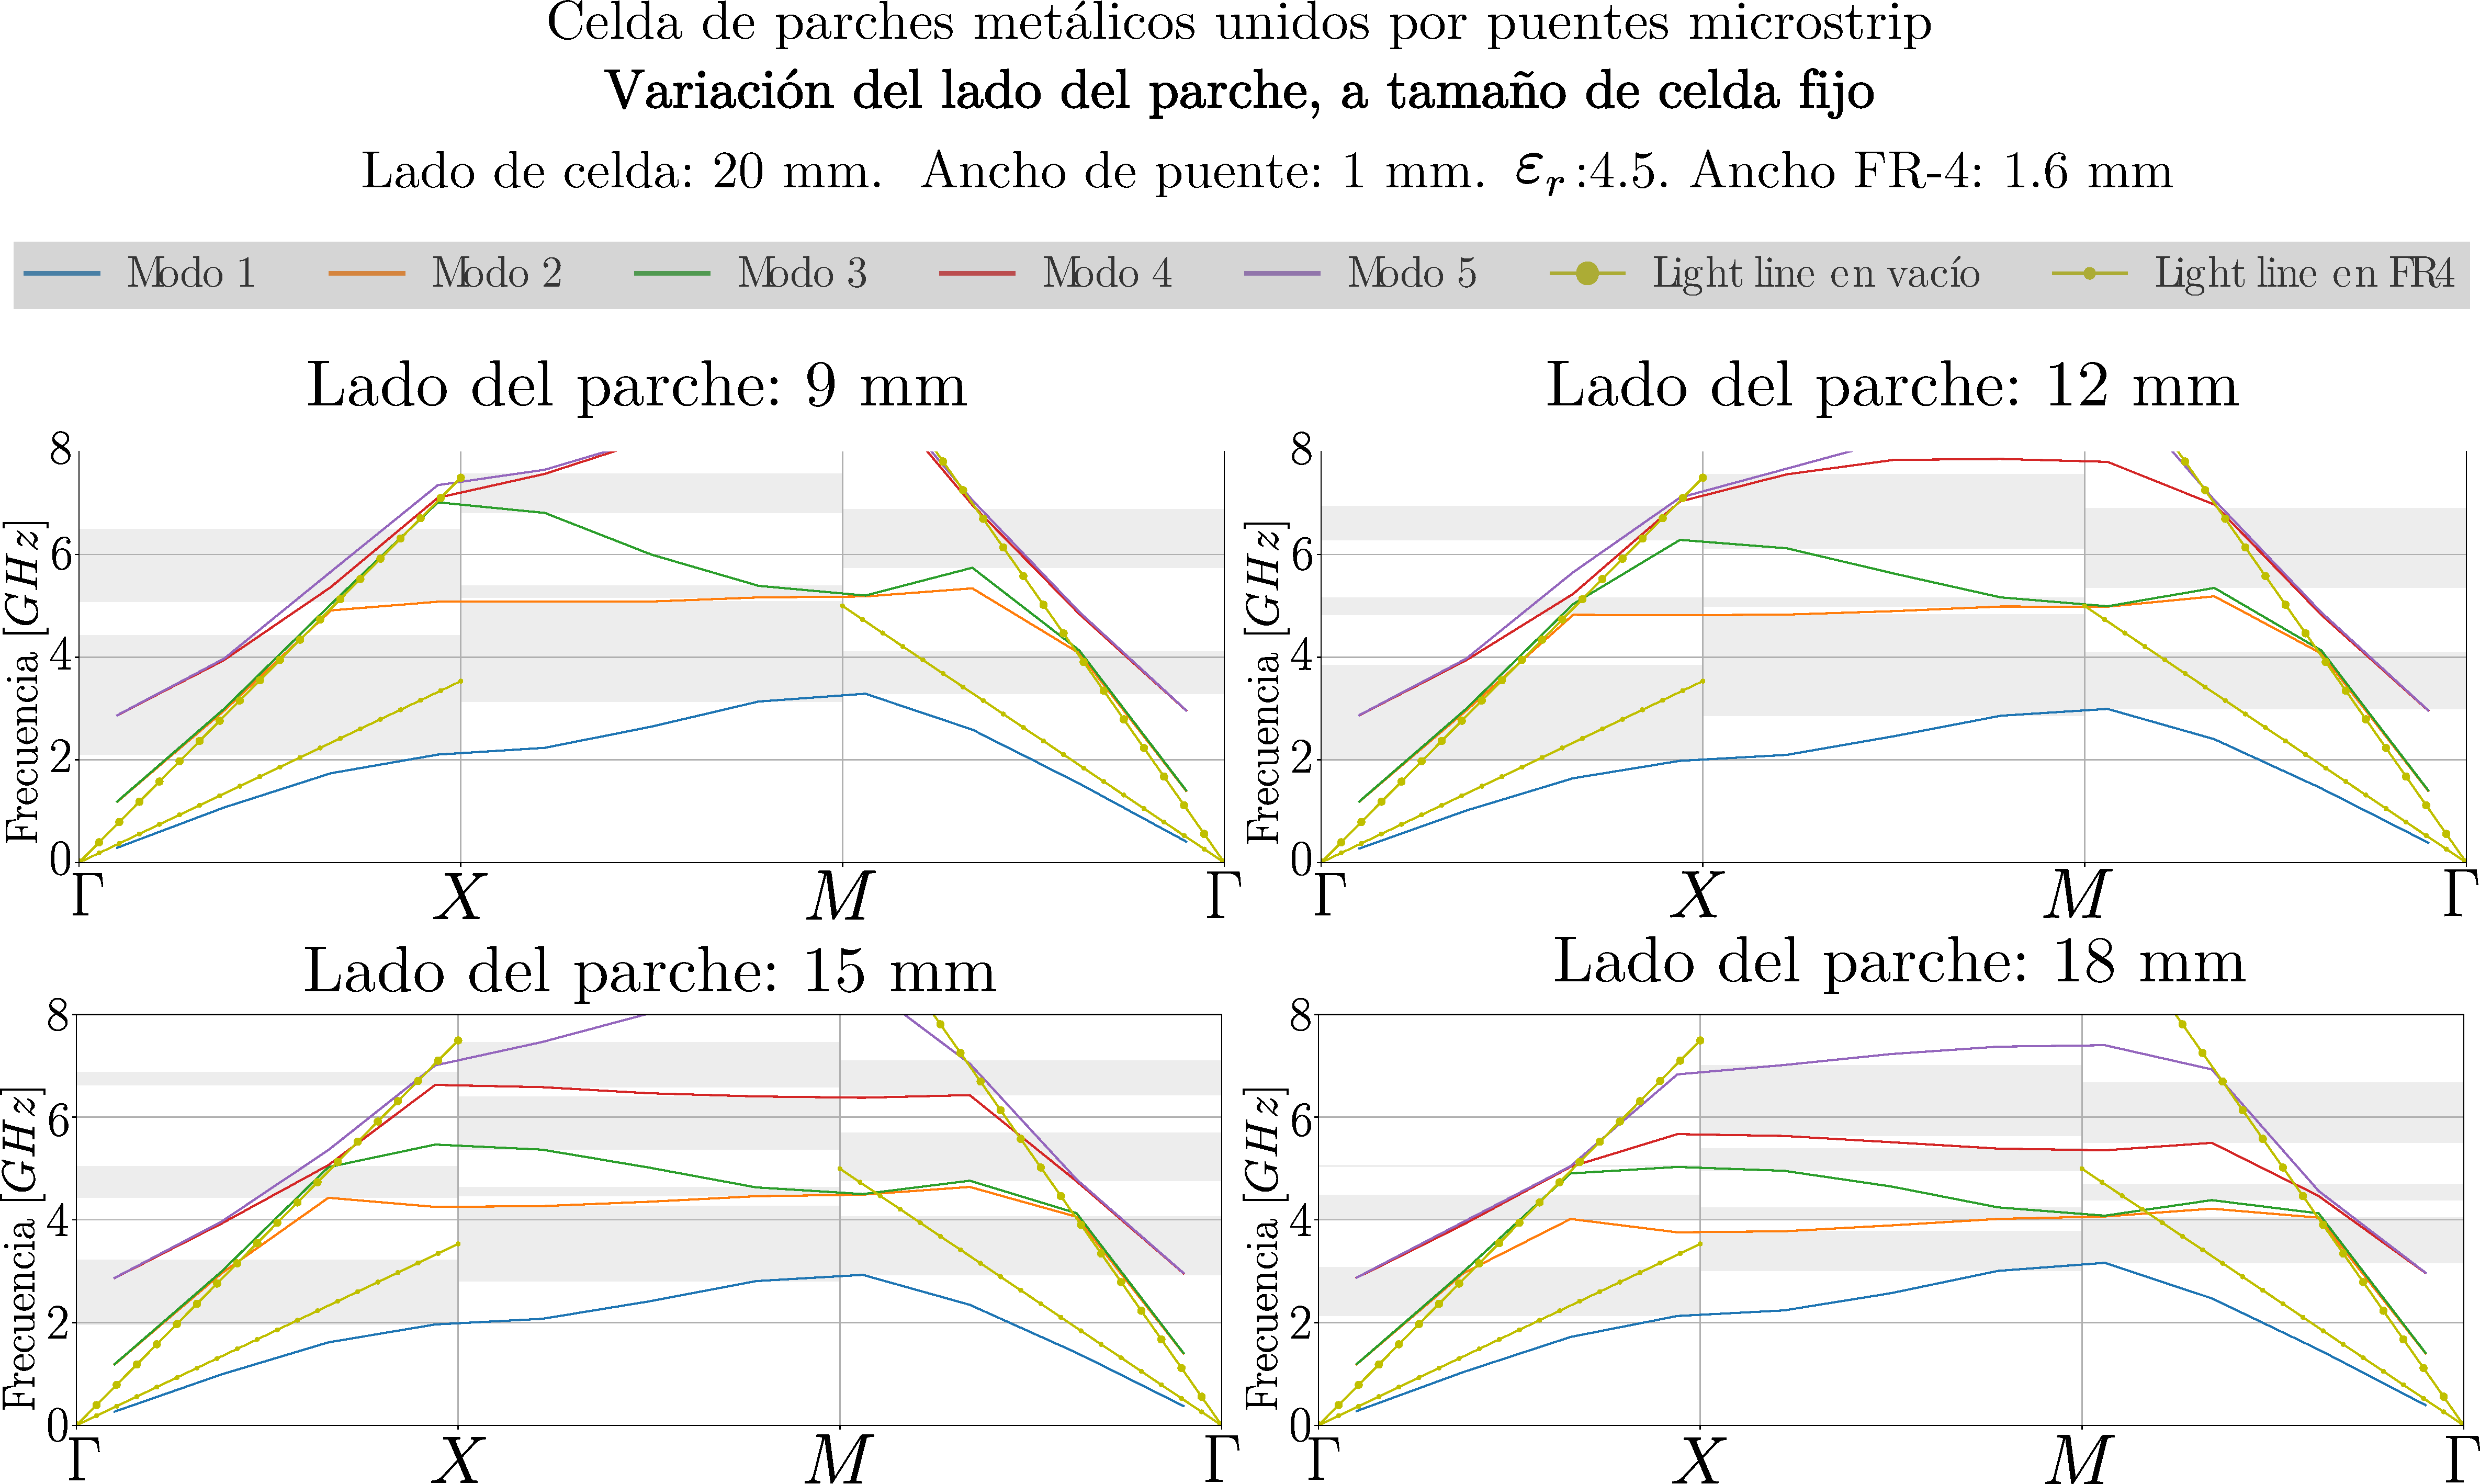
\includegraphics[width=1\textwidth]{Modelado/Orlandi-DeltaParcheMetalicoCeldaFija.pdf}
	\caption{Diagramas de dispersión para la variación del tamaño del parche metálico, sin una variación en el tamaño de la celda unitaria. El sustrato de FR-4 de $1.6\;\text{mm}$ de espesor.}
	\label{fig:diagdisp-orlandi-variacion-tam-parche}
\end{figure}


\begin{figure}[h]
	\centering
	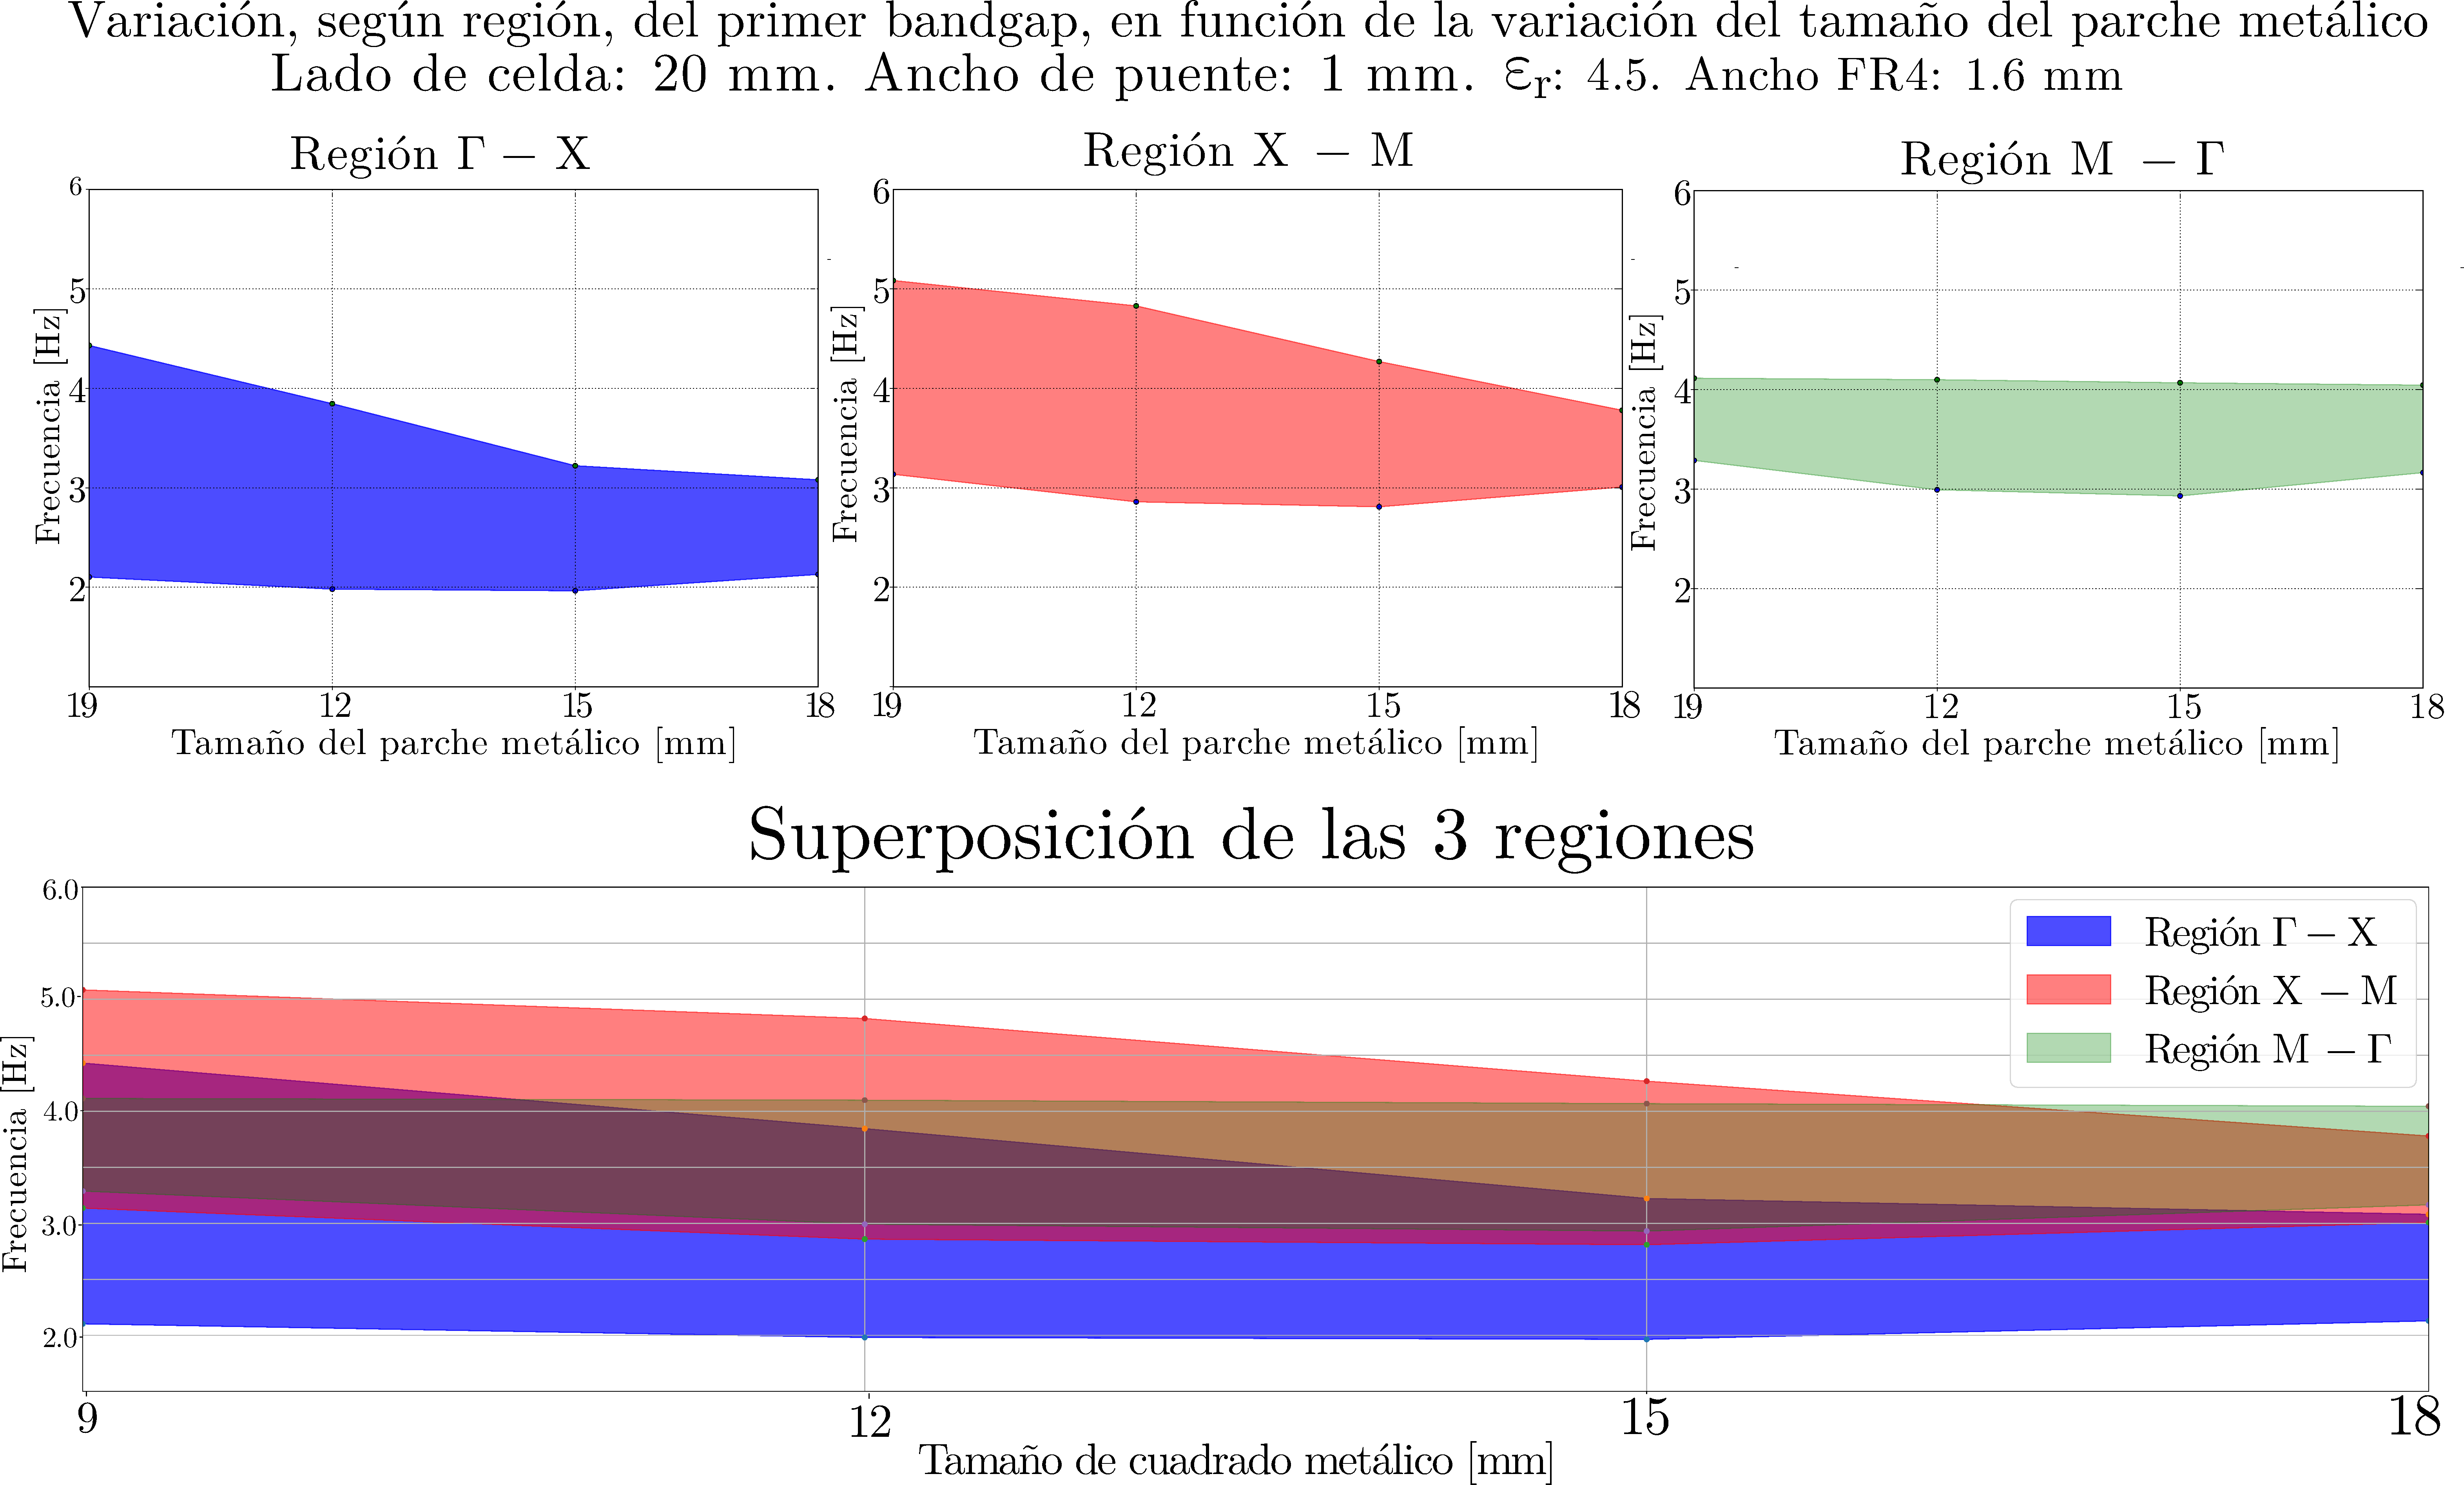
\includegraphics[width=1\textwidth]{Modelado/Orlandi-DeltaParcheMetalicoCeldaFija-Comparacion.pdf}
	\caption{Compraración del ancho del primer band-gap (entre el primer y el segundo modo de propagación) para las tres direcciones analizadas, en función del tamaño del parche.}
	\label{fig:comparacion-diagdisp-orlandi-variacion-tam-parche}
\end{figure}

La figura \ref{fig:diagdisp-orlandi-variacion-tam-parche} muestra que, al contrario que en el caso anterior, la mera variación del tamaño del parche metálico, sin la modificación del tamaño de la celda unitaria, no genera los mismos efectos. La variación de la capacidad, como antes, da lugar a una disminución en la frecuencia central del primer \textit{bandgap}.

Por otro lado, la inductancia impuesta por los puentes disminuye considerablemente cuando el tamaño del parche aumenta sin que lo haya la celda unitaria en general. En este sentido, manteniendo la analogía con el filtro LC presentado antes, dado que el ancho de banda de resonancia de un filtro LC es aproxidamente $BW_r \approx \sqrt{L/C}$, si disminuye el valor de la inductancia (por puentes más cortos) y, al mismo tiempo, aumenta el valor de la capacidad (por el aumento del efecto de capacitor de placas planas paralelas y las capacidades mutuas entre celdas vecinas) , el ancho de banda disminuirá notablemente.

Como se puede ver en la figura \ref{fig:comparacion-diagdisp-orlandi-variacion-tam-parche}, un mayor ancho de banda prohibida se obtiene con parches de tamaño moderado, con los que además es posible obtener bandas prohibidas completas.


\subsubsection{Variación de la longitud de los puentes}


\begin{figure}[h]
	\centering
	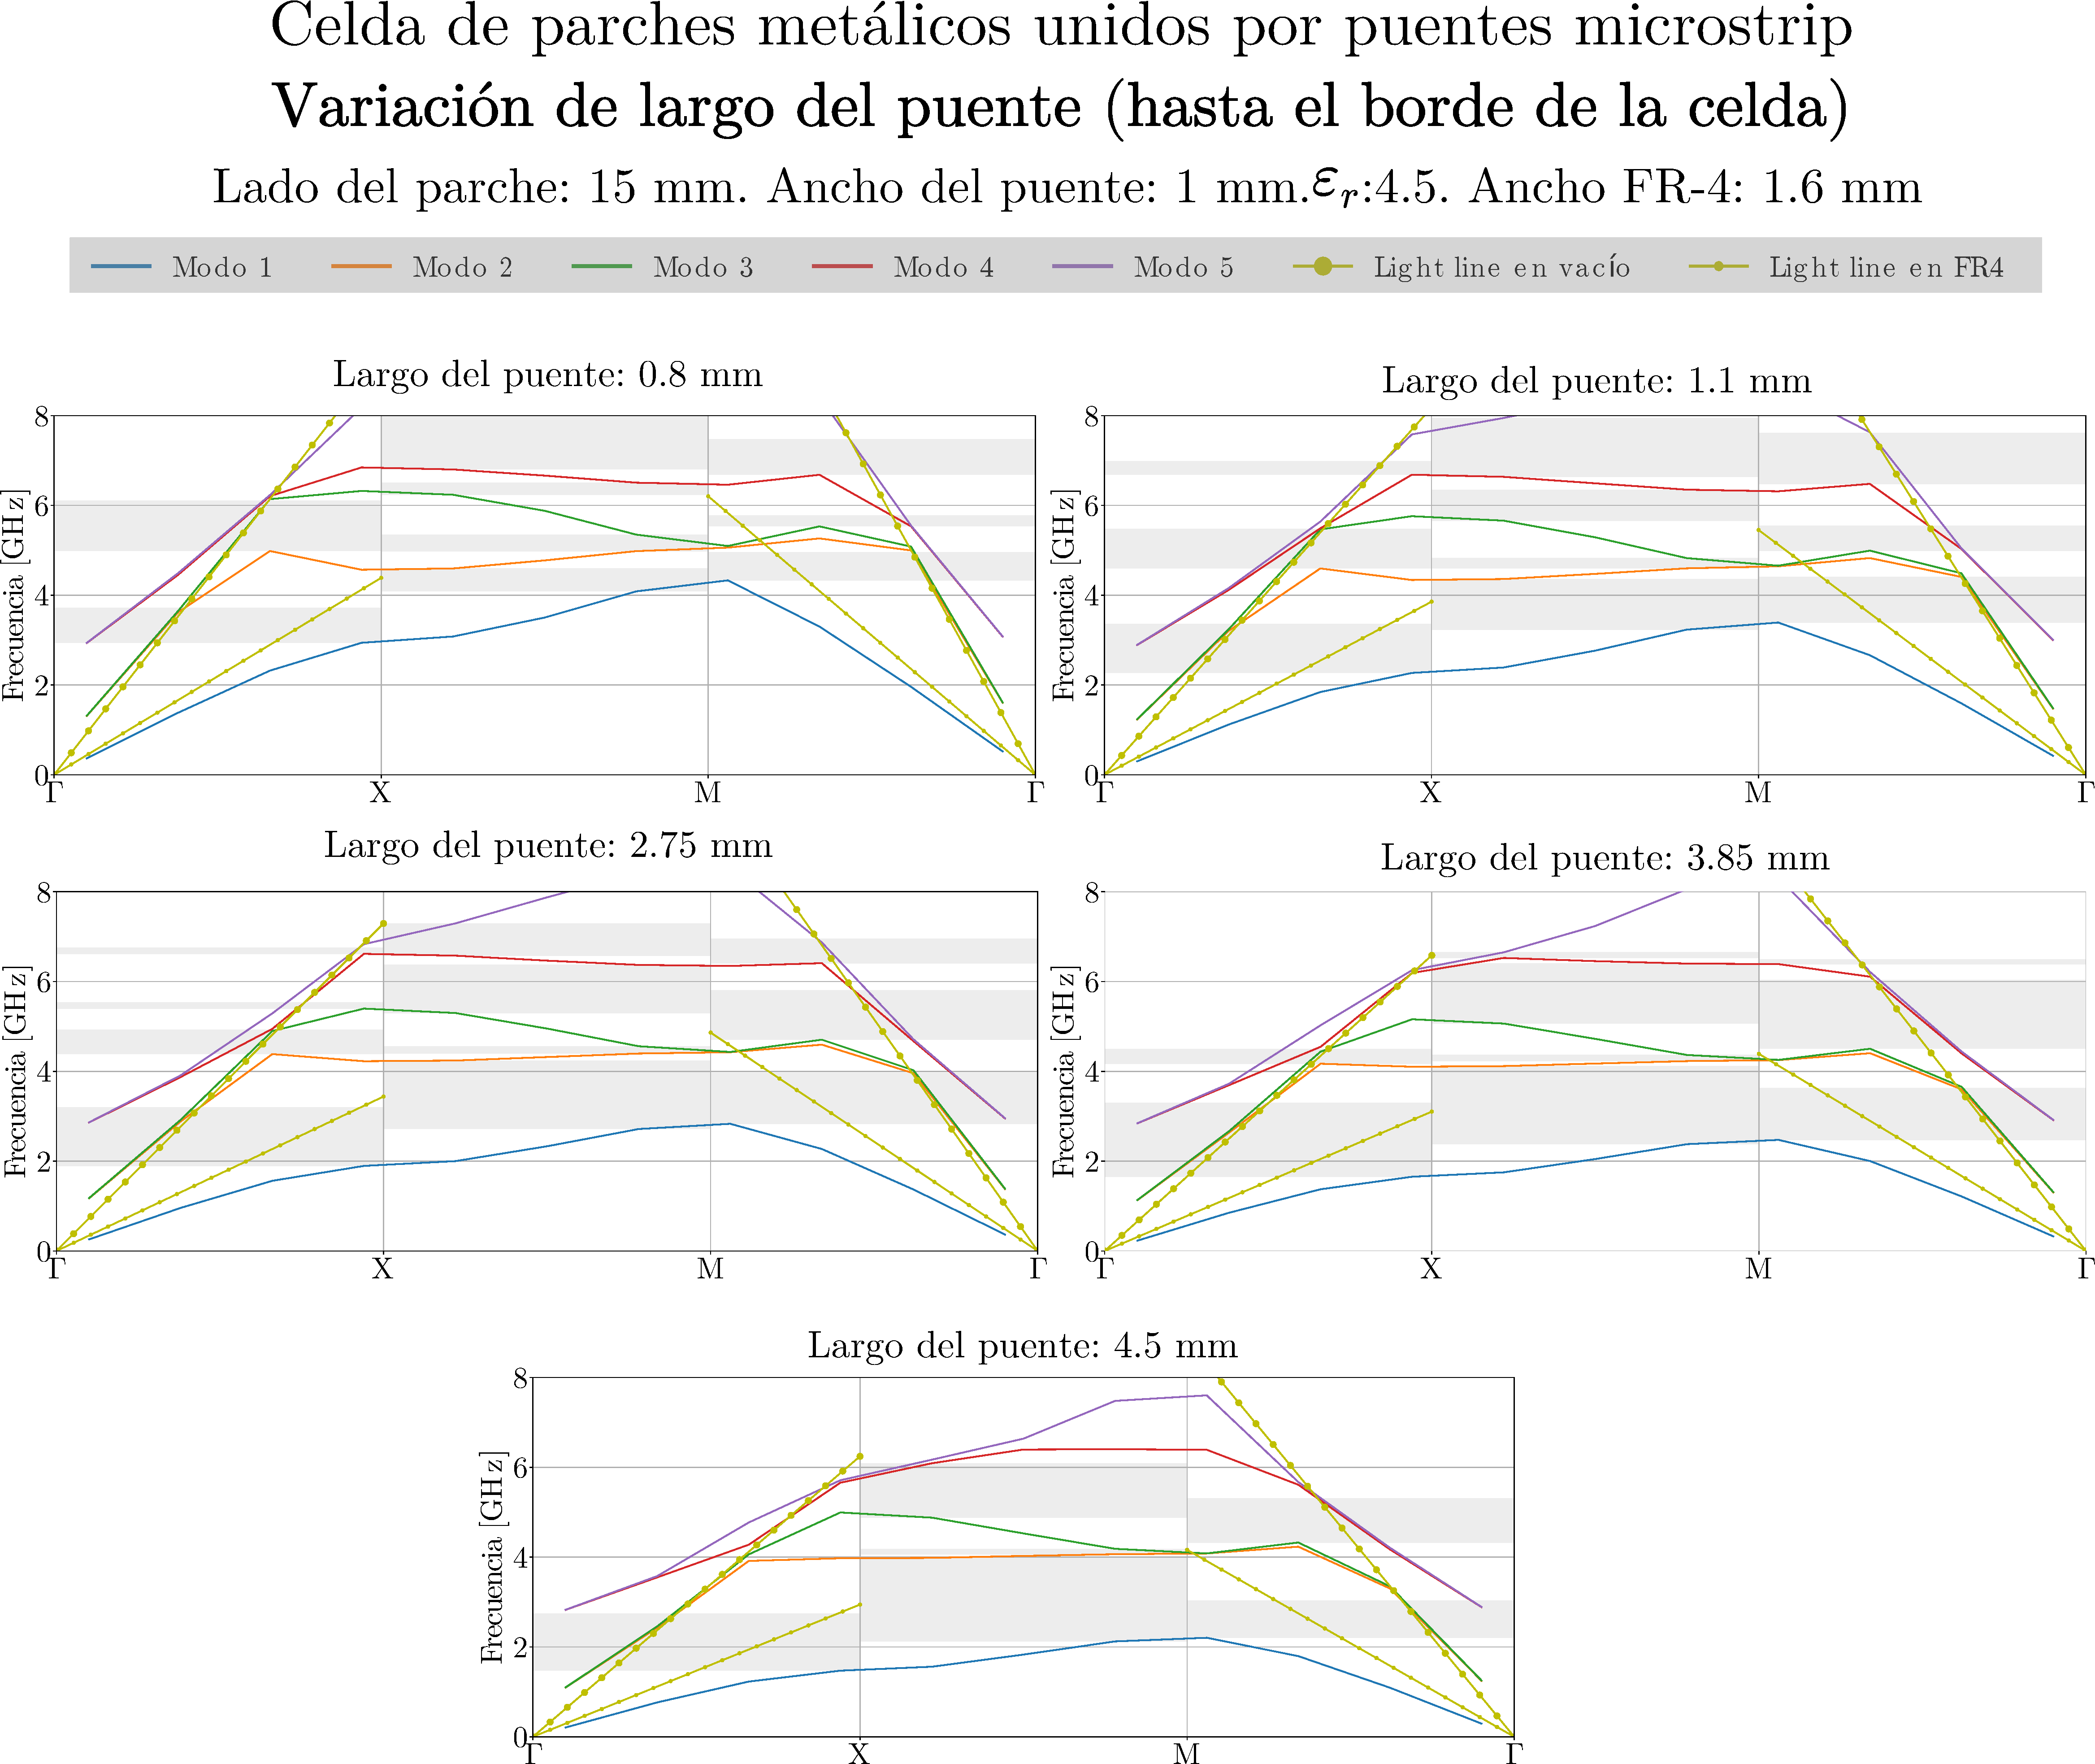
\includegraphics[width=1\textwidth]{Modelado/Orlandi-DeltaSeparacionParches-DeltaTamanioCelda-ParcheFijo.pdf}
	\caption{Diagramas de dispersión para la variación del largo de los puentes, que equivale a un aumento del tamaño de la celda unitaria, si las dimensiones del parche \textit{microstrip} se mantienen fijas. El sustrato de FR-4 de $1.6\;\text{mm}$ de espesor.}
	\label{fig:diagdisp-orlandi-variacion-long-puentes}
\end{figure}



\begin{figure}[h]
	\centering
	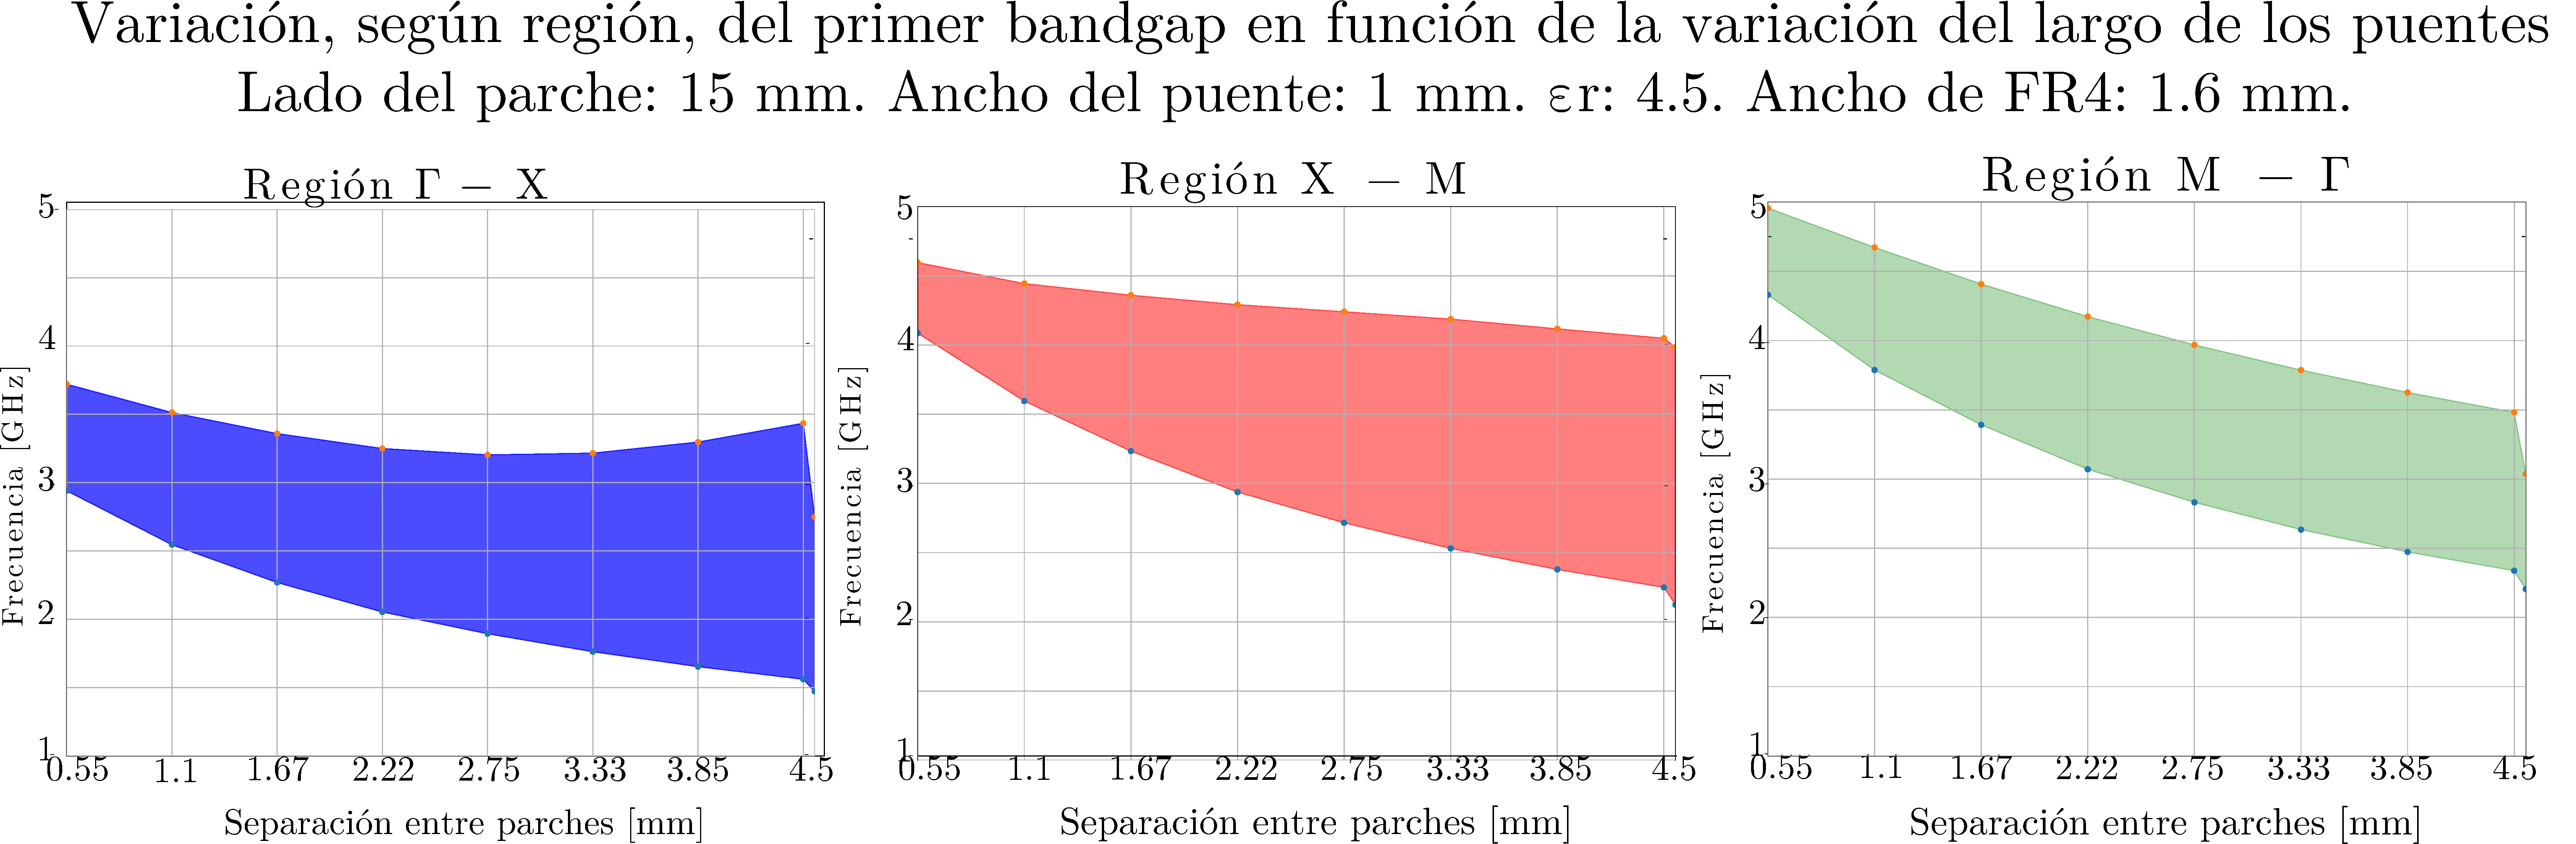
\includegraphics[width=1\textwidth]{Modelado/Orlandi-DeltaSeparacionParches-DeltaTamanioCelda-ParcheFijo-Comparacion.pdf}
	\caption{Compraración del ancho del primer band-gap (entre el primer y el segundo modo de propagación) para las tres direcciones analizadas, en función del largo de los puentes que unen a los parches.}
	\label{fig:comparacion-diagdisp-orlandi-long-puentes}
\end{figure}


Para la variación de la longitud de los puentes es necesario, nuevamente, modificar el tamaño de la celda unitaria, por lo que, necesariamente, a medida que exista una mayor separación entre los parches (y por tanto una mayor longitud de puentes), la frecuencia central de la banda prohibida disminuirá.

Por otro lado, dado que la capacidad no cambiará (excepto aquella correspondiente al efecto de capacidad entre parches cercanos, que estarán cada vez más alejados), los efectos más notorios, bajo un análisis cuasiestático, se darán por el aumento de la inductancia. El alejamiento de los parches metálicos entre sí disminuirá la capacidad total de cada celda unitaria, pero los efectos no son lo suficientemente notorios. Si los puentes no exisitieran, el efecto sería el opuesto al que se da en esta geometría \cite{Yang:EBGAntennas}. Este aumento en la inductancia generará un mayor ancho de banda, que se ve reflejado en la figura \ref{fig:comparacion-diagdisp-orlandi-long-puentes}.

\subsubsection{Efecto de la variación del ancho del sustrato dieléctrico}

\begin{figure}[h]
	\centering
	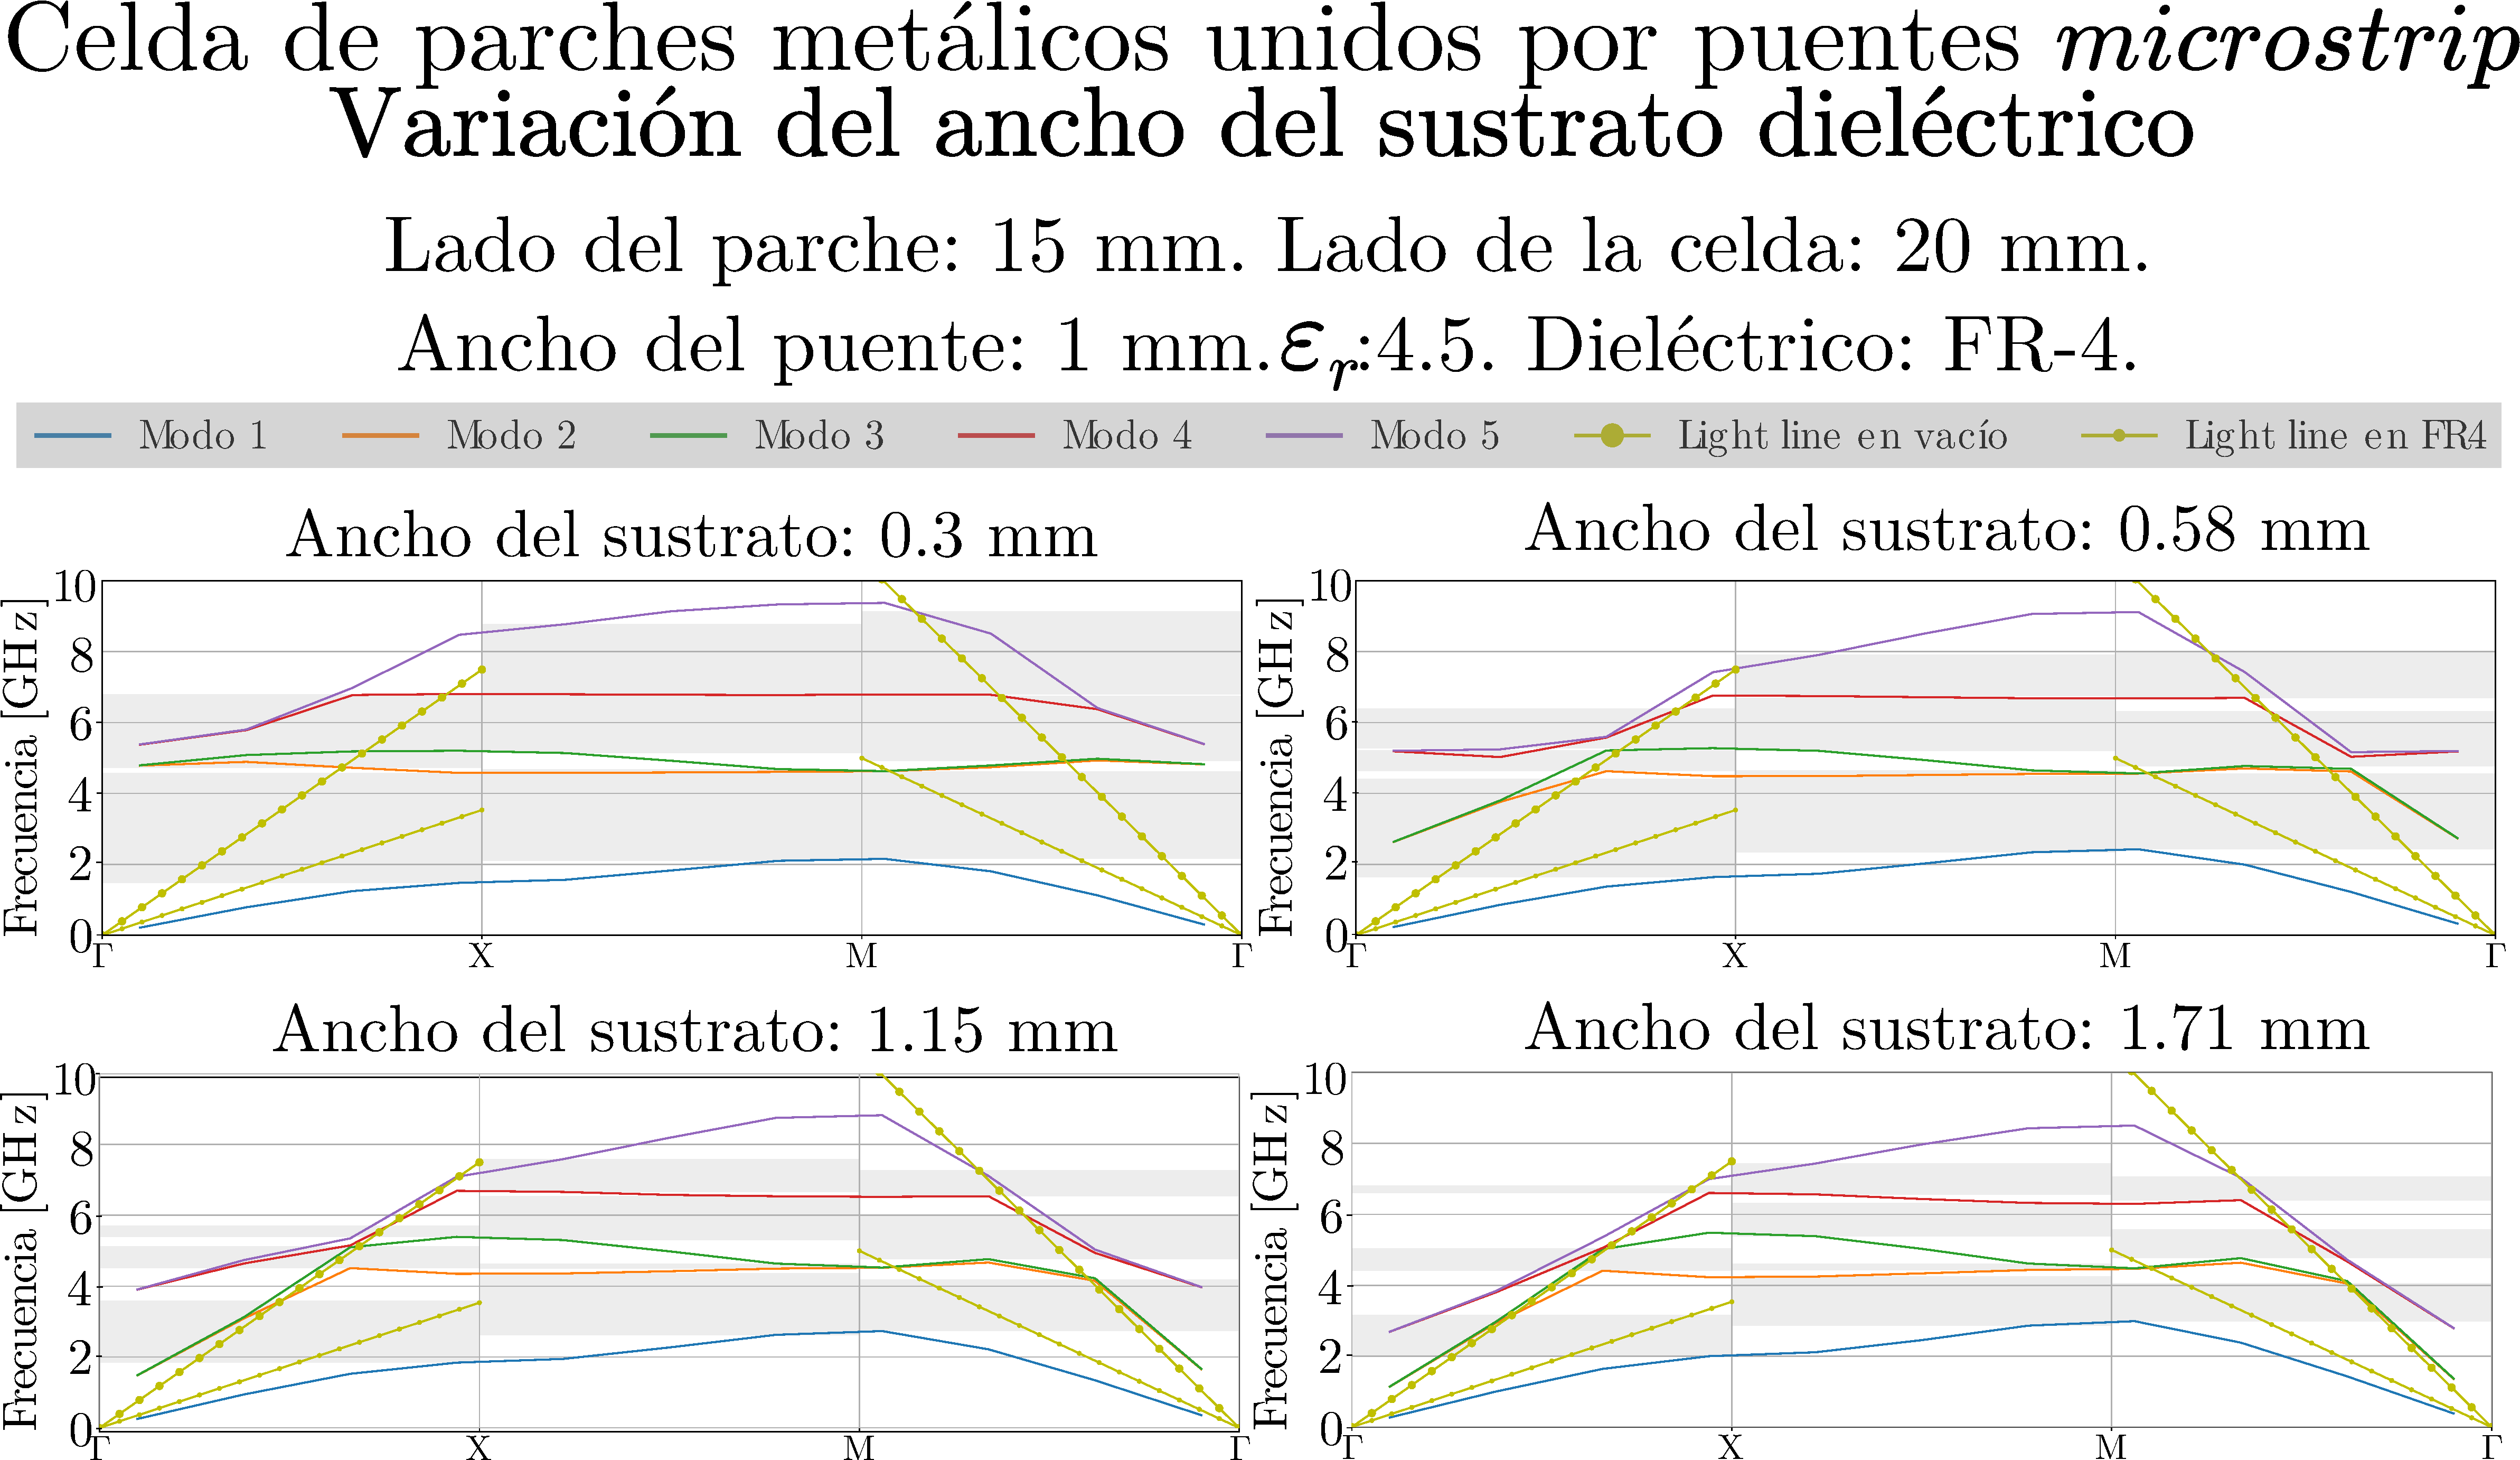
\includegraphics[width=1\textwidth]{Modelado/Orlandi-DeltaAnchoSustrato.pdf}
	\caption{Diagramas de dispersión para la variación del ancho del sustrato dieléctrico. El sustrato de FR-4 de $1.6\;\text{mm}$ de espesor.}
	\label{fig:diagdisp-orlandi-variacion-ancho-diel}
\end{figure}


\begin{figure}[h]
	\centering
	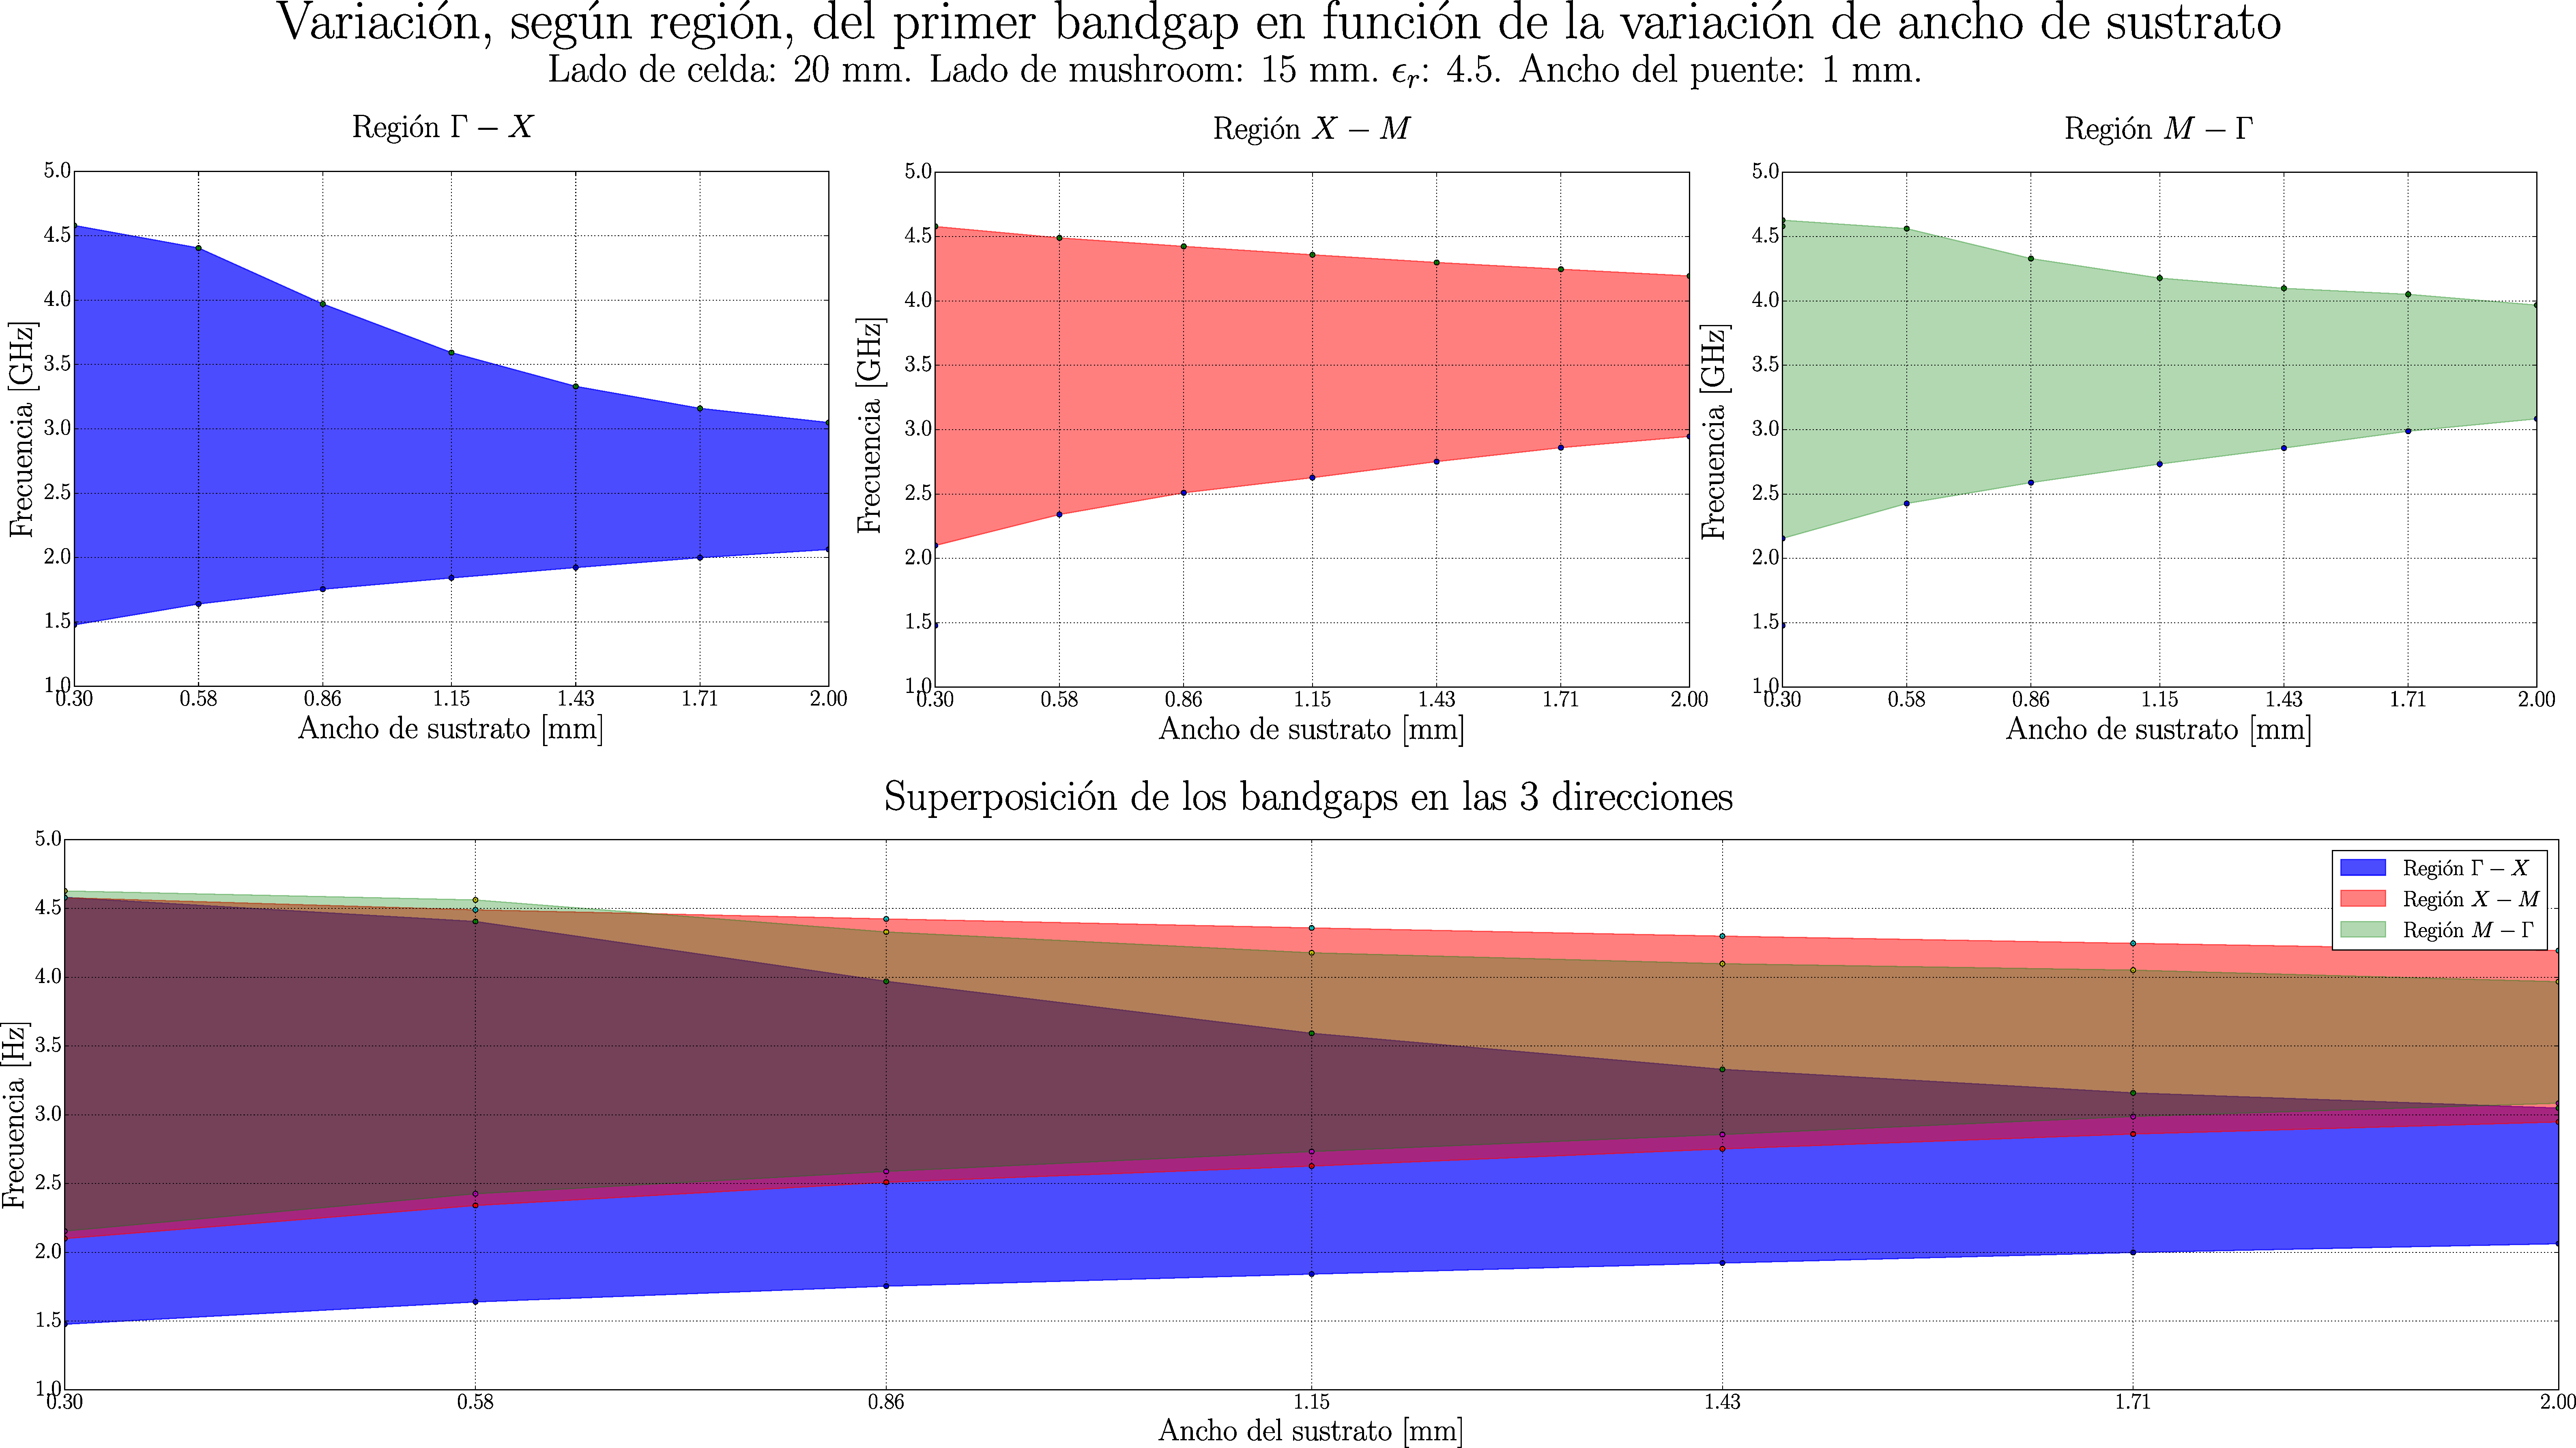
\includegraphics[width=1\textwidth]{Modelado/Orlandi-3direcciones-anchoSustrato-Comparacion.pdf}
	\caption{Comparación del ancho del primer band-gap (entre el primer y el segundo modo de propagación) para las tres direcciones analizadas, en función del ancho del sustrato dieléctrico.}
	\label{fig:comparacion-diagdisp-orlandi-variacion-ancho-diel}
\end{figure}

La variación del ancho del sustrato tiene importantes consecuencias en el EBG. Por un lado, es importante notar que el comportamiento del ancho de banda es opuesto al que se obtiene considerando el modelo cuasiestático: Un aumento en la capacidad (debido al acercamiento de los planos paralelos que forman los parches y el plano conductor inferior, cuando disminuye el ancho del sustrato), debería dar lugar a una disminución notoria en el ancho de banda. Sin embargo, como se observa en la figura \ref{fig:comparacion-diagdisp-orlandi-variacion-ancho-diel}, se da el efecto contrario.

El comportamiento resulta más intuitivo si se recuerda que, como se explicó en la sección \ref{cap_intro_electro}, un sustrato delgado dificulta la aparición de ondas de superficie, volviendo a las zonas prohibidas de propagación más notorias.

A medida que aumenta el tamaño del mismo, disminuye el ancho de banda de la zona prohibida, y resulta más dificultoso obtener un \textit{bandgap} completo.

\clearpage

\subsection{Celda de Yang}
\label{sec:celda-yang}

La búsqueda de estructuras que requirieran un menor tamaño de celda unitaria para lograr zonas prohibidas en frecuencias bajas, impulsó a Fei-Ran Yang, Kuang-Ping Ma, Yongxi Qian y Tatsuo Itoh, en 1991, a presentar \cite{Yang:UCPBG} la geometría mostrada en la figura \ref{fig:celda-yang}. En la misma, como se puede observar, se intentó maximizar la longitud de los puentes, estableciendo lo que se conoce como un \textit{inset} en el parche \textit{microstrip}. De esta forma, el parche puede crecer, y por tanto aumentar la capacidad, sin que por ello la inductancia deba disminuir. Esto permite, además, que los parches de las distintas celdas unitarias se ubiquen a corta distancia unos de otros, aumentando entonces el acoplamiento capacitivo entre ellos, y por tanto la capacidad del sistema completo. A pesar de las modificaciones, la simetría se mantuvo, por lo que las rectas de análisis de la zona irreducible de Brillouin son las mismas que para el caso de la celda analizada en la sección \ref{sec:celdas-orlandi}.

\begin{figure}[h]
	\centering
	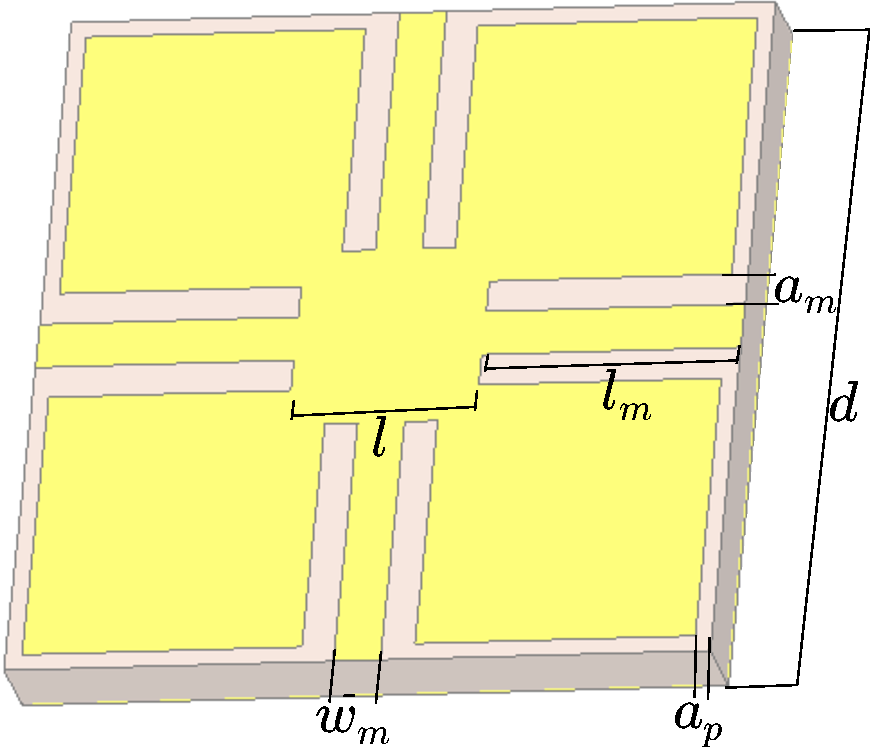
\includegraphics[width=0.4\textwidth]{Modelado/yang-celda.pdf}
	\caption{Celda unitaria del metamaterial presentado en 1999 por Yang, Ma, Qian e Itoh.}
	\label{fig:celda-yang}
\end{figure}

Aplicando, nuevamente el análisis de autovalores con condiciones de borde periódicas, se puede observar el comportamiento de los campos, más complejo que en la celda unitaria analizada antes. El mismo se muestra en la figura \ref{fig:yang-analisis-campos}.

Para el primer modo de propagación, resuelta evidente que, como en la estructura de parches cuadrados unidos por puentes analizada antes, el campo eléctrico es principalmente normal al plano sobre el que se ubica la estructura, y se ubica mayormente bajo el parche, donde se presenta el efecto de placas planas paralelas. Sin embargo, debido  a que ahora los puentes parten desde el interior del parche, existen también componentes tangenciales a la superficie. Estas componentes, como se puede observar en la figura \ref{fig:yang-analisis-campos} b) (para el primer modo) y f) (para el segundo modo), son muy notorias en los bordes de la celda unidad, por lo que los efectos de acoplamiento capacitivo mutuo entre celdas son mucho más notorios que en la celda analizada antes.

\begin{figure}[h]
	\centering
	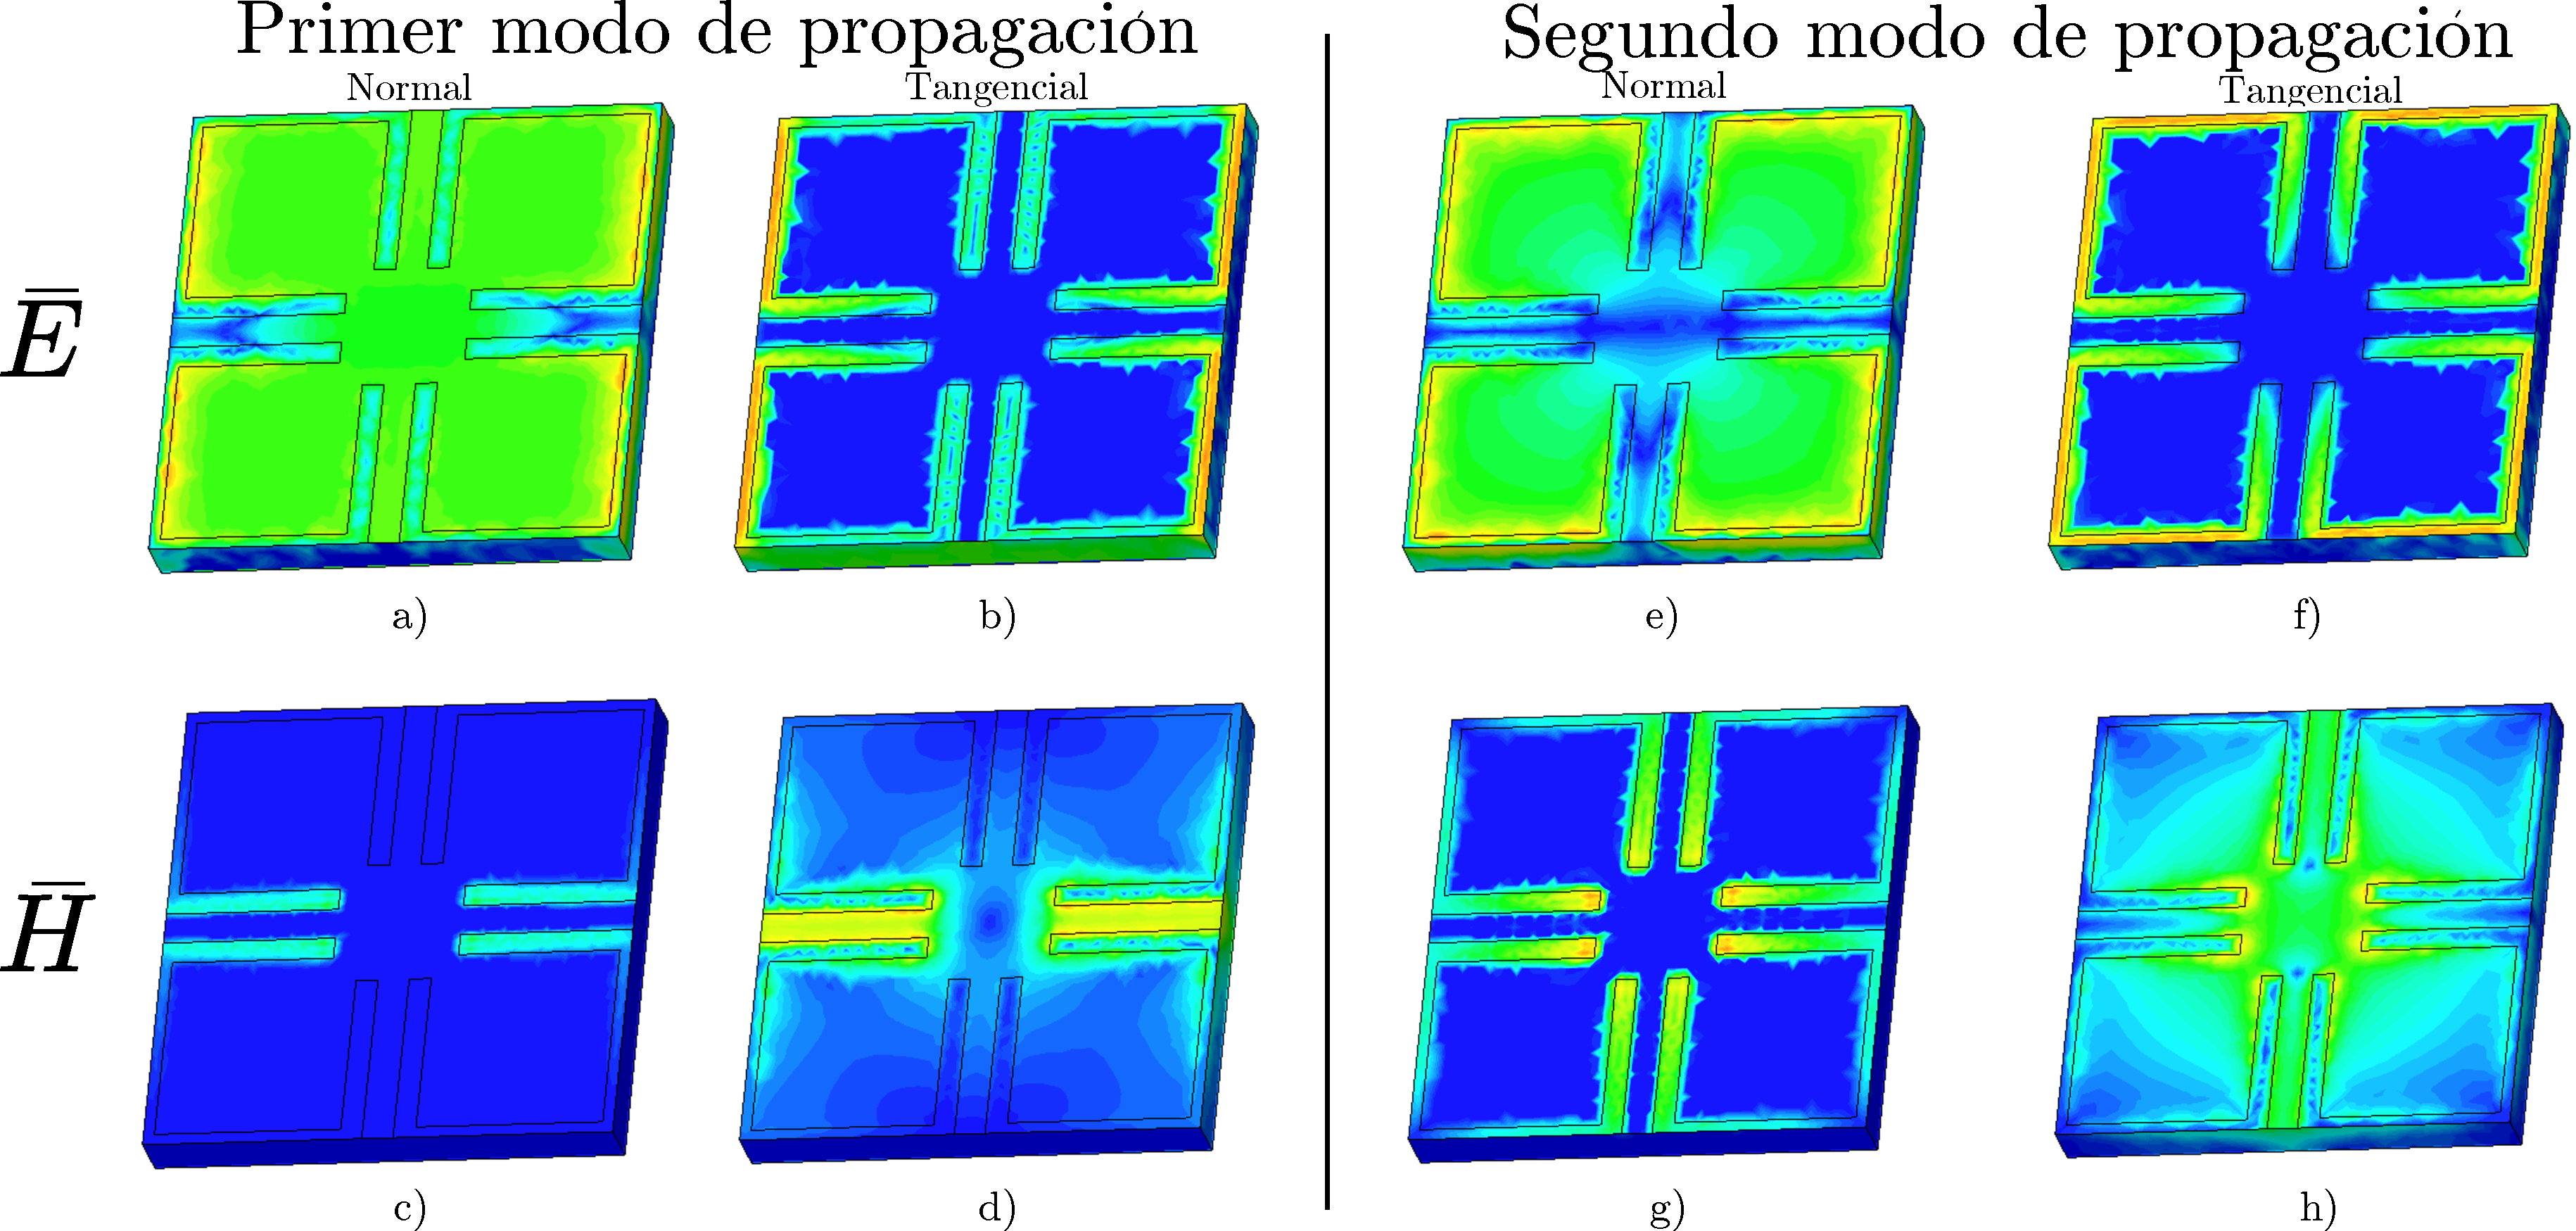
\includegraphics[width=1\textwidth]{Modelado/yang-modo1-Enorma-Etangencial.pdf}
	\caption{Comportamiento, en promedio temporal, de los campos eléctrico y magnético sobre una celda unitaria de Yang, para el primer y segundo modo de propagación.}
	\label{fig:yang-analisis-campos}
\end{figure}

Los campos magnéticos, por otro lado, para el primer modo de propagación son muy similares a los que presenta la celda analizada antes, incluyendo su variación temporal, que puede verse en las figuras \ref{fig:yang-analisis-campos-fases} c) y d) para dos tiempos distintos dentro del periodo. En el primero de ellos, cuando el campo eléctrico tiene amplitud máxima sobre el parche (figura a)), la corriente saliente al parche a través de los puentes horizontales crece. De la misma forma, cuando la tensión en el parche decrece a su mínimo, la corriente entrante al parche es máxima.

Para el segundo modo de propagación, el campo eléctrico, en promedio (figura \ref{fig:yang-analisis-campos} e) y f)) tiene un comportamiento muy similar al primer modo de propagación, pero como se puede observar en las figuras correspondientes de la figura \ref{fig:yang-analisis-campos-fases}, para tiempos distintos, el campo es mayor, alternadamente, en la parte superior e inferior de los parches. El campo magnético normal a superficie, en promedio, se puede observar, para este modo de propagación, presente en todas las aperturas metálicas de la celda unidad, indicando que sobre los parches y los bordes del parche circula una corriente notoria. En las figuras \ref{fig:yang-analisis-campos-fases} g) y h) se puede observar el campo magnético para dos momentos de tiempo distinto. Este campo magnético sugiere que en los puentes horizontales hay corrientes en ambas direcciones en todo momento (debido a que las dos aperturas que lo rodean presentan un campo magnético normal saliente), mientras que los puentes verticales poseen corrientes en un único sentido y, al contrario que para el caso de los puentes horizontales del primer modo, en este caso el sentido es el mismo.

\begin{figure}[h]
	\centering
	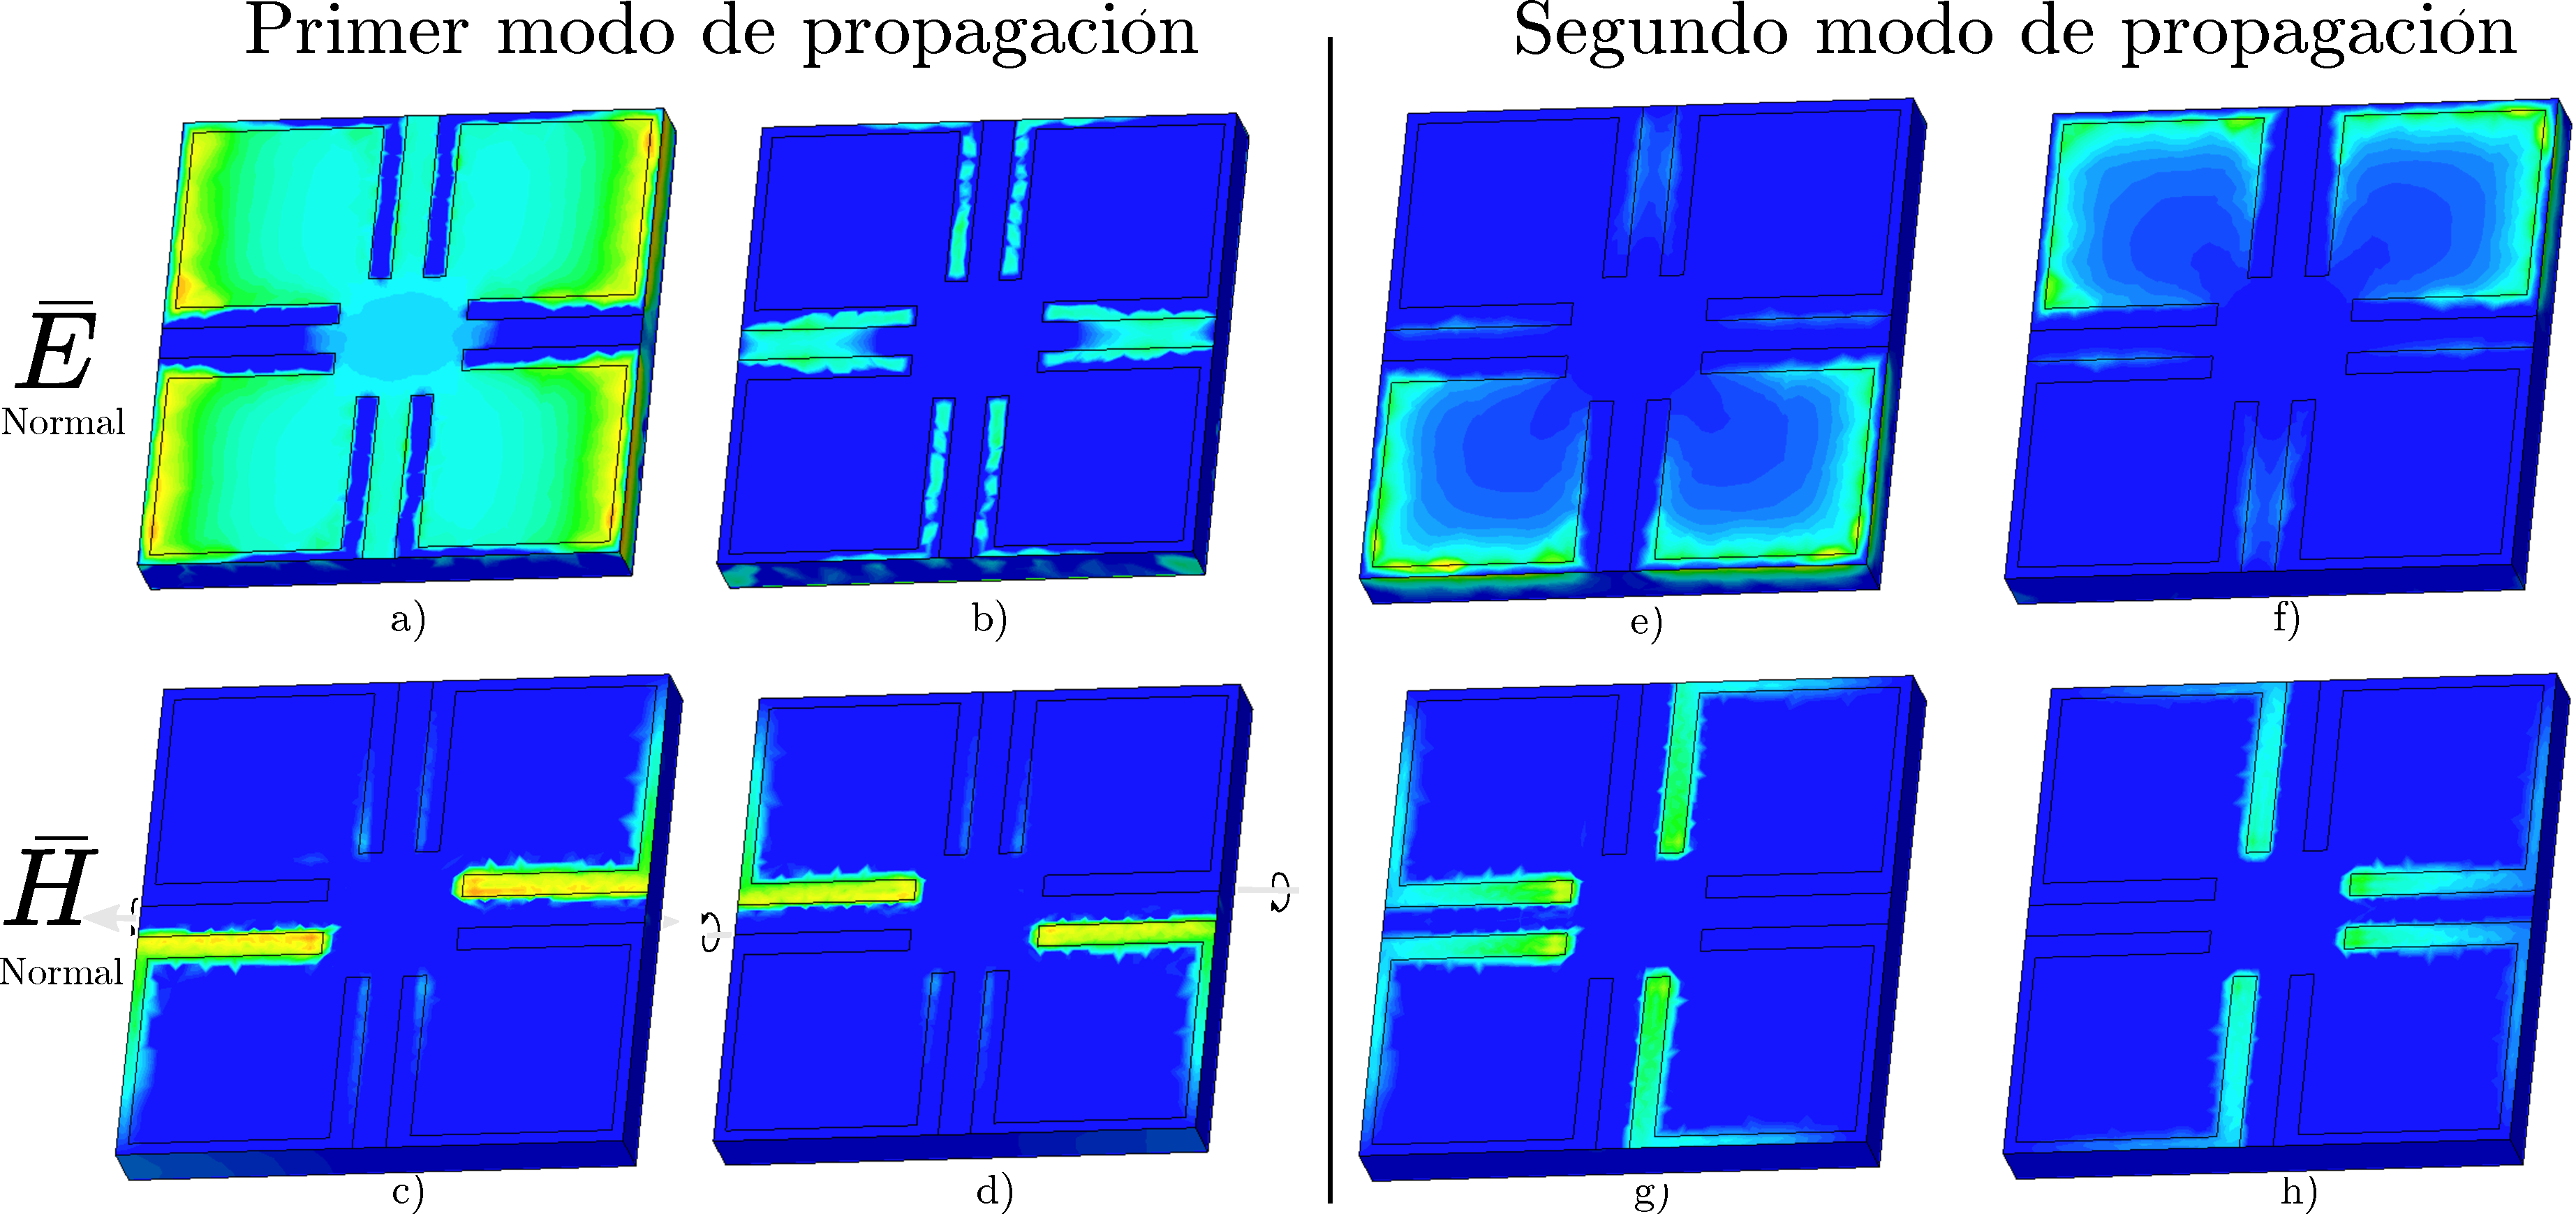
\includegraphics[width=1\textwidth]{Modelado/yang-modo1-EH-fases.pdf}
	\caption{Comportamiento, para dos tiempos diferentes, de los campos eléctrico y magnético normales a la superficie, sobre la celda propuesta por Yang, Ma, Qian e Itoh, para el primer y segundo modo de propagación.}
	\label{fig:yang-analisis-campos-fases}
\end{figure}


Se debe tener en cuenta que el uso de esta estructura presenta mayores dificultades, especialmente cuando su construcción se realiza por técnicas rudimentarias. Sin embargo, gracias a un mejor aprovechamiento del espacio, que permiten obtener una mayor capacidad e inductancia por celda unitaria, la geometría permite diseñar celdas unitarias más pequeñas para lograr zonas prohibidas para frecuencias de microondas que las que se pueden lograr utilizando la geometría analizada en la sección \ref{sec:celda-orlandi}.

\section{Modelado circuital}

La forma más sencilla de modelar el comportamiento resonante es la representación circuital, como la discutida en la sección \ref{sec:modelo_analitico}. En la misma deben intervenir capacitores e inductores con valores seleccionados en función del comportamiento de la energía en la estructura. Si bien los efectos de altas frecuencias no podrán ser analizados bajo esta representación, sí debería ser posible observar, al menos en forma general, los fenómenos analizados para las frecuencias de trabajo, de manera que se pueda realizar una acercamiento intuitivo y conceptual al problema.

Para el caso particular de la celda de Yang presentada en la sección \ref{sec:celda-yang}, a raíz de la visualización del comportamiento de los campos, resulta fácil comprender que, si bien los fenómenos que intervienen son numerosos, los más importantes están fuertemente vinculados a la circulación de corriente por el puente y al desarrollo del campo eléctrico entre las celdas.

Se propusieron distintos circuitos, de diversa complejidad, para representar a cada celda unitaria propuesta por Yang, basados principalmente en el circuito mostrado en la figura \ref{fig:circuito-equivalente-kim-parches} y se analizaron los parámetros S21 de cada uno, en vistas de lograr un comportamiento similar al obtenido cuando se utiliza el software CST Microwave Studio para simular la estructura. El primero de los circuitos propuestos se puede observar en la figura \ref{fig:primerCircuitoPropuesto}. En el mismo se intentó utilizar la estructura LC paralela resonante para obtener un bandgap para el rango de frecuencias estudiado.

La estructura LC paralela posee una frecuencia de resonancia en $f=1/(2 \pi \sqrt{LC})$, en la que abandona su comportamiento inductivo, y adopta un comportamiento predominantemente capacitivo. Para esa frecuencia, existe un intercambio de energía entre el inductor y el capacitor, de forma que la impedancia de entrada presenta un máximo. A esta frecuencia, entonces, el circuito se comporta como un filtro de tipo notch, que podría explicar parte del comportamiento de bandgap en microondas.

Los valores geométricos de la celda unitaria utilizada como testigo son los que se muestran en la tabla \ref{table:CeldaUnitariaAnalisisiCircuital}, en función de los valores descriptos en la figura \ref{fig:primerCircuitoPropuesto}. Se consideró la permitividad relativa del FR-4, de 4.4.

\begin{tabular}{|c|c|c|c|c|c|}
	\label{table:CeldaUnitariaAnalisisiCircuital}
	\hline 
	$d$ & $l$ & $w$ & $d_l$ & $g$ & $h$ & $d_w$\\ 
	\hline 
	$22.6\;mm$ & $6\;mm$ & $1.1\;mm$ & $0.8\;mm$ & $0.8\;mm$ & $1.6\;mm$ & $16.6\;mm$\\ 
	\hline 
\end{tabular} 

La inductancia parcial del puente, $L_b$, se obtiene en base a 3 cálculos independientes, provenientes de modelos distintos de comportamiento de estructuras \textit{microstrip}. El primero de ellos es el mostrado en la ecuación \ref{eq:cgap-y-lgap}, repetido en la ecuación \ref{eq:lbridge1-circuital} por comodidad.

\begin{equation}
\label{eq:lbridge1-circuital}
L_{b} = 0.2\; \text{nH/mm} \cdot \ln (2\pi \frac{h}{w}).
\end{equation}

El segundo método es el propuesto por C. Paul en \cite{CPaul:InductanceLoopAndPartial}:

\begin{equation}
\label{eq:lbridge2-circuital-cpaul}
L_{b} = \begin{cases}
			\frac{60 l}{c} \ln \left( \frac{8h}{w} + \frac{w}{4h} \right) \text{ para } \frac{w}{h}\leq 1\\
			\frac{120 \pi l}{c} \frac{1}{w/h+1.393+0.667\ln(w/h+1.444)} \text{ para } \frac{w}{h} \g 1 \\
		\end{cases}
\end{equation}

Por último, la inductancia parcial se calculó utilizando el software Ansys Q3D Extractor de Ansoft, que realiza simulaciones cuasiestáticas utilizando el método BEM (\textit{Boundary Element Method}), basado en la resolución de las funciones de Green, y que por lo tanto sólo requiere la discretización de la fuente de campo, y no del espacio circundante.

Los valores de $L_b$ obtenidos se muestran en la tabla \ref{table:Lb}.

\begin{tabular}{|c|c|c|}
	\label{table:Lb}
	\hline 
	Método 1 & Método 2 & Método 3\\ 
	\hline 
	$7.34\;nH$ & $8.2\;nH$ & $7.7\;nH$\\ 
	\hline 
\end{tabular}

El valor de la capacidad entre las protuberancias de las celdas unitarias, $C_g$, se calculó utilizando la expresión de la ecuación \ref{eq:lbridge1-circuital}, repetida aquí por comodidad, y bajo la nomenclatura del problema:

\begin{equation}
\label{eq:cgap1-circuital}
C_{g} = \frac{d_w\epsilon_0(1+\epsilon_r)}{\pi}\cosh^{-1}(\frac{2 d_w + g}{g}).
\end{equation}

Además, se utilizó también Q3D Extractor para obtener un valor aproximado de capacidad entre dos celdas unitarias, utilizando la geometría mostrada en la figura \ref{fig:capacidad-cg-Q3D}. Se consideró, tanto en la ecuación \ref{eq:cgap1-circuital} como en la simulación, que la principal responsabilidad por la capacidad entre celdas vecinas recae sobre las esquinas más próximas de las celdas unitarias. Además, para la simulación fue necesario eliminar el puente \textit{microstrip} que las conectaba, debido a que, dado que la simulación es cuasiestática, si el conductor es el mismo, la capacidad resulta nula.

\begin{figure}[h]
	\centering
	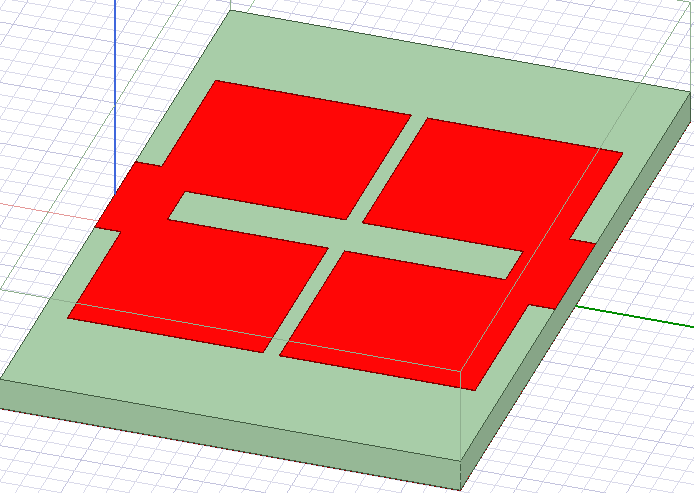
\includegraphics[width=1\textwidth]{Modelado/capacidad-cg-Q3D.png}
	\caption{Geometría utilizada para calcular la capacidad entre celdas vecinas con Q3D Extractor.}
	\label{fig:capacidad-cg-Q3D}
\end{figure}

\begin{tabular}{|c|c|c|}
	\label{table:Lb}
	\hline 
	Aproximación matemática & Simulación \\ 
	\hline 
	$475 fF\;$ & $211 fF$\\ 
	\hline 
\end{tabular}

Se observa que los valores son disímiles entre sí, por lo que, en el circuito, el valor de esta capacidad deberá ser obtenido por deducción en base al comportamiento en frecuencia, manteniendo estos valores como referencia.


\section{Modelado por líneas de transmisión}
%%%%

Además del acercamiento a través del uso de circuitos equivalentes de primer orden, en general es posible expresar el problema a partir de su generalización como un conjunto de líneas de transmisión efectivas (en lugar de líneas de transmisión propiamente dichas), discretizando el espacio de forma que cada paso de discretización resulte mucho menor a $\lambda/4$ \cite{Caloz:ElectromagneticMetamaterials}, aproximadamente. Este acercamiento, y el uso de líneas de transmisión generalizadas (donde se pueden considerar capacidades en serie e inductancias en paralelo) resultan útiles para describir distintos tipos de metamateriales, incluyendo aquellos que son conocidos como ``de mano izquierda" \cite{Caloz:ElectromagneticMetamaterials}.

Para el caso bidimensional, la discretización debe ser también bidimensional, lo que conlleva mayores esfuerzos numéricos. Un problema práctico cualquiera puede contener una enorme cantidad de celdas unitarias, con bordes complejos y medios inhomogéneos, lo que obliga a considerar las propiedades de las celdas unitarias de la forma lo más sencilla posible, y para aumentar la densidad de las mismas con el menor impacto posible en el tiempo de procesamiento.

Existen numerosos métodos que utilizan líneas de transmisión para simular metamateriales, entre los que destacan el método de TMM (\textit{Transmission-Matrix Method}) y de TLM (\textit{Transmission-Line Matrix Method}). Si bien los nombres son similares, la resolución del problema varía fundamentalmente \cite{Caloz:ElectromagneticMetamaterials}. En este trabajo se desarrollará brevemente el método de TLM, que luego será implementado y explicado en detalle en la sección \ref{subsec_estudio_tlm}.

El método de matrices\footnote{Aquí el término matrices se refiere a un arreglo bidimensional, y no a un objeto matemático.} de líneas de transmisión consiste en la discretización espacial del problema físico en pequeñas subceldas. El comportamiento de los campos electromagnéticos en las mismas se concentra en un nodo o punto en el espacio, y las relaciones de adyacencia entre ellas se modelan utilizando líneas de transmisión que vinculan los nodos. Estas líneas son capaces de transmitir impulsos cortos sin distorsión, y de distribuirlos, en cada uno de los nodos, de acuerdo a un algoritmo local para cada subcelda \cite{Caloz:ElectromagneticMetamaterials}, hacia cada uno de los nodos adyacentes. Este algoritmo local no es más que la multiplicación del pulso incidente por los parámetros S de transmisión y reflexión en cada tiempo, que se pueden obtener a partir del análisis de la celda y sus vecinas. De esta manera, se discretiza un circuito equivalente al problema físico a resolver, y se simula la propagación de ondas electromagnéticas a partir del \textit{scattering} de impulsos en una red n-dimensional de nodos unidos por lineas de transmisión.

El algoritmo fue propuesto inicialmente en 1971 por Johns y Beurle \cite{JohnsBeurle:TLM}, y provee soluciones en el dominio del tiempo, a partir del estudio de la propagación de impulsos electromagnéticos muy cortos en las estructuras. La información en el dominio de la frecuencia se obtiene realizando una transformada de Fourier\footnote{Numéricamente, se suele realizar una transformada discreta de Fourier, cuya implementación más conocida es la Fast Fourier Transform (FFT)} de la respuesta de la red al impulso, como en todo método numérico en el dominio del tiempo. Esta metodología lo vuelve útil especialmente para aplicaciones de gran ancho de banda, donde se desea obtener características en un amplio rango de frecuencias con una única simulación.

El método fue generalizado, más tarde, al estudio de estructuras tridimensionales, donde se reemplazaron los conceptos de capacidad e inductancia de la línea de transmisión, por parámetros físicos del medio. En general, la capacidad e inductancia asociadas a las líneas de transmisión que unen los nodos que representan un medio en particular son elegidas de forma que la impedancia característica coincida con la impedancia intrínseca del mismo. En general, las pérdidas en el medio se tienen en cuenta a partir del uso de resistencias, o la aplicación de una constante de atenuación en cada cálculo de \textit{scattering} sobre los nodos.

% Cuentas! Wu, Lin, Wang, Wang, Chen

%%%%
\subsection{Algoritmo utilizando programación orientada a objetos}
\label{subsec_estudio_tlm}
%%%%
La simulación se corre a través de un \textit{script} editable de Python, donde se establecen las condiciones de la simulación en forma manual, y se determina si se leerán resultados calculados previamente o se calcularán nuevos. En el mismo, además, se permite elegir si se considerarán  las capacidades de acople entre elementos, la cantidad de tiempos a simular y las frecuencias superior e inferior de análisis. Se debe tener en cuenta, además, que se especifica la discretización espacial (cantidad de milímetros de cada estructura simulada, denominada \textit{Pixel}). La discretización espacial se relaciona con la temporal, dado que en TLM están vinculadas por la velocidad de propagación de una onda electromagnética en el medio. Así, la primera deberá asegurar que la segunda permita cumplir con las condiciones del teorema de Nyquist para la caracterización de las señales calculadas (esto significa que, dado que la velocidad de propagación, $v_p=\frac{\Delta l}{\Delta t}$ relaciona las discretizaciones espacial y temporal, la discretización espacial debe ser tal que $\Delta l = v_p \frac{\Delta t}{2}$ para cumplir las condiciones del teorema de Nyquist, lo que deriva en que $\Delta l = \frac{v_p}{2f}$, con $f$ la frecuencia de interés, que en nuestro caso es $2.4\;\text{GHz}$).

\begin{figure}[h]
	\centering
	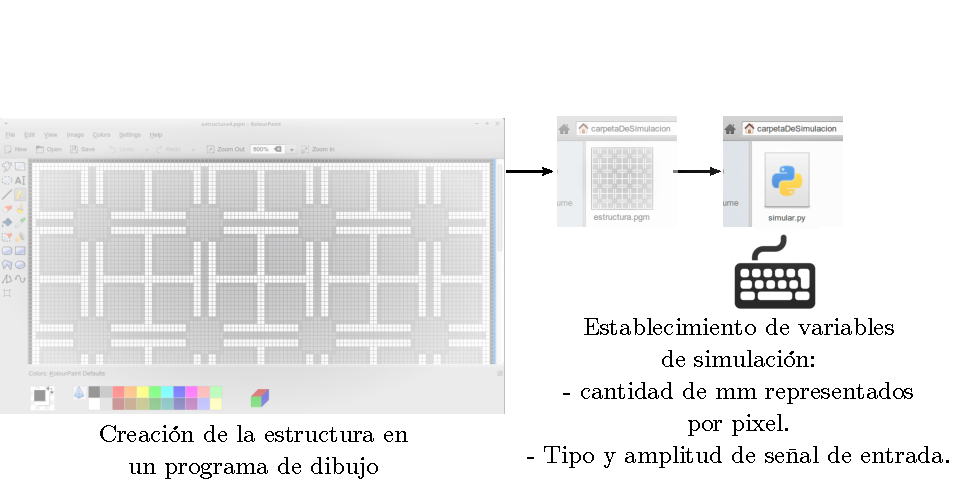
\includegraphics[width=\textwidth]{Modelado/ProcedimientoUsuario.pdf}
	\caption{Esquema de ingreso de datos al simulador.}
	\label{fig:esquema-ingreso-datos}
\end{figure}

Como se esquematiza en la figura \ref{fig:esquema-ingreso-datos}, la entrada de datos se realiza a través de un archivo con formato \textsc{.PGM} ASCII\footnote{El formato PGM es un antiguo formato de almacenamiento de imágenes en escala de grises. Estos archivos pueden ser modificados por programas de edición de imágenes, como Microsoft Paint y Kolourpaint, y además por editores de texto plano. Cuando se utiliza uno de estos últimos, se observa que las primeras líneas indican la cantidad de filas ($n$) y columnas ($m$) en que se disponen los pixeles de la imagen, y luego la lista de valores entre 1 y 255 que indican la opacidad/claridad del pixel. Los primeros $m$ valores corresponden a los pixeles, de izquierda a derecha, que corresponden a la primer fila; los siguientes $m$ valores corresponden a la segunda fila, etc.}, que establece una matriz de \textit{pixeles}, cada uno con un valor, entre 1 y 255, donde 1 representa el negro, 255 el blanco, y los valores intermedios corresponden a una escala de grises. El archivo se puede generar a partir de un programa de edición de imágenes, lo que facilita la creación de estructuras a simular, ya que la misma sólo debe ser dibujada con la resolución requerida. Si la imagen creada ocupa una mayor cantidad de \textit{pixeles} (tiene una mayor resolución), la granularidad espacial utilizada en la simulación será mayor, dado que existe una relación 1 a 1 entre la densidad de \textit{pixeles} gráficos y la discretización utilizada, lo que significa que la discretización es realizada por el usuario en el momento de crear la imagen, y el mallado es rectangular y estático.

La lectura de la imagen del disco genera un objeto \textit{Superficie}, que almacena, en forma ordenada, los \textit{Pixeles} dibujados, que son objetos con características eléctricas variables, en función de su color en la imagen, como se muestra en la figura \ref{fig:tiposdepixeles}. En la misma se pueden observar 4 tipos de \textit{pixeles}:

\begin{figure}[h]
	\centering
	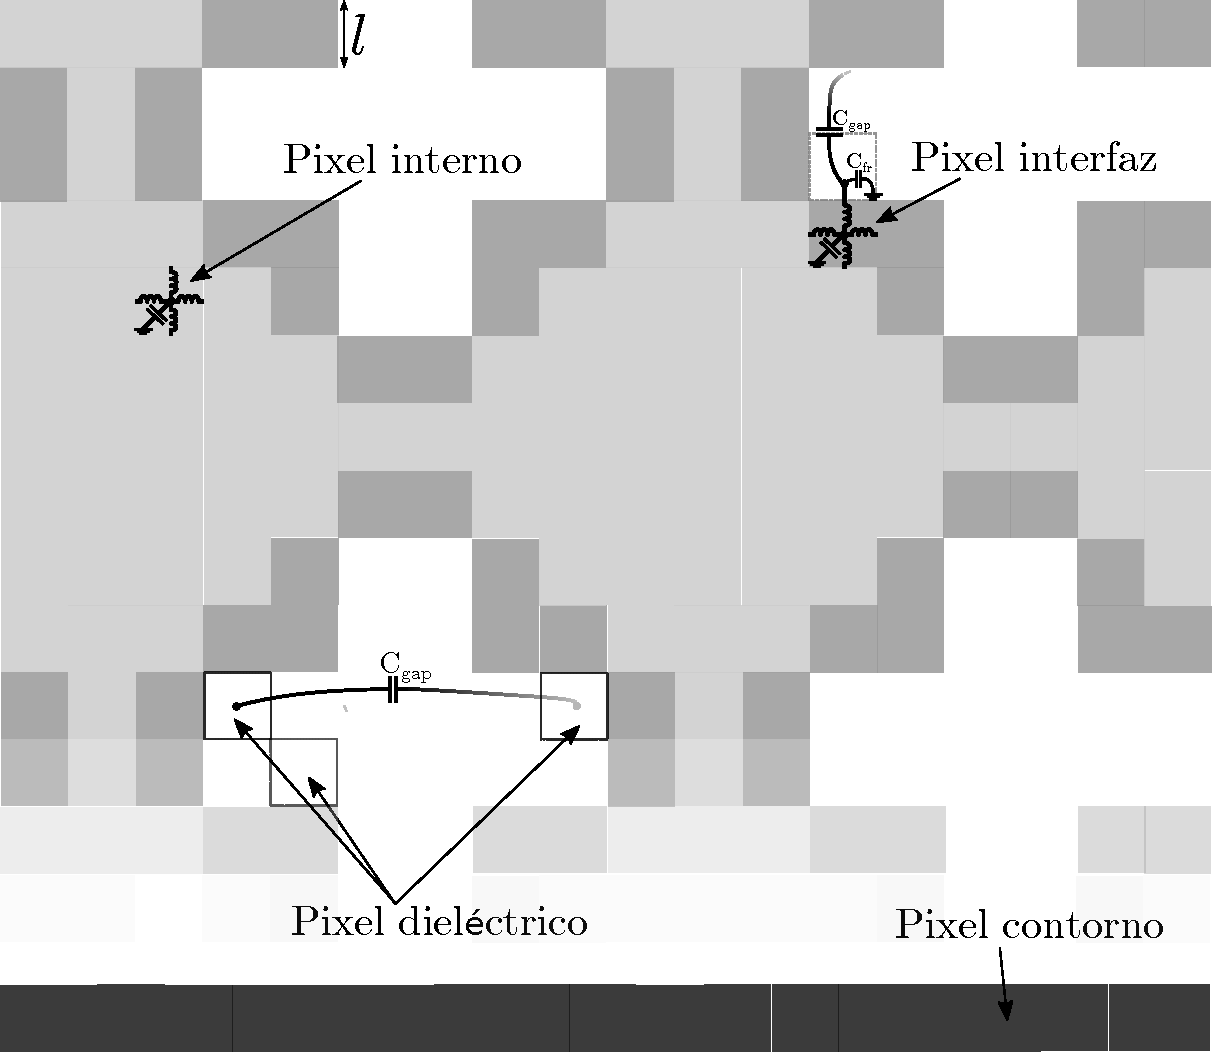
\includegraphics[width=\textwidth]{Modelado/TiposDePixel.pdf}
	\caption{Circuitos equivalentes propuestos para cada tipo de pixel.}
	\label{fig:tiposdepixeles}
\end{figure}

\begin{enumerate}
	\item \textbf{Interno}. Representan superficies metálicas que se encuentran en el interior de un plano conductor.
	\item \textbf{Interfaz}. Representan superficies metálicas que se encuentran en los bordes de una estructura metálica, lo que significa que tienen vecinos que son otros \textit{pixeles} de tipo metálico (de interfaz o internos) y vecinos dieléctricos. Son los \textit{pixeles} que poseen la propiedad de capacidad de \textit{fringe}.
	\item \textbf{Dieléctricos}. Representan las zonas donde no hay cobre, sino simplemente dieléctrico desnudo (en particular, FR-4). Estos \textit{pixeles} no participan del intercambio de energía en el modelo.
	\item \textbf{Contorno}. Pueden intentar simular una superficie perfectamente adaptada, o una superficie metálica, en función de las necesidades de la simulación. Se ubican en el borde de la imagen \textsc{.pgm} creada, para que actúen como el borde del espacio de simulación.
\end{enumerate}


Una vez cargada la imagen en memoria, creado el objeto \textit{Superficie} y los objetos \textit{Pixeles}, se los vincula.

Como se observa en la figura \ref{fig:tiposdepixeles}, los pixeles metálicos (internos y de interfaz) tienen una capacidad y varias inductancias asociadas (una para cada dirección). Las mismas quedan descriptas en base a las ecuaciones \ref{eq:Cp_Lp}, y a partir de ellas es posible obtener una impedancia característica, como se muestra en la figura \ref{fig:modelo-con-lineas-de-transmision}, en base a las ecuaciones \ref{eq:capacidad-inductancia-impedancia-modelado}:

\begin{subequations}
	\label{eq:capacidad-inductancia-impedancia-modelado}
	\begin{align}
		L_{inn} &= \mu_0 h /2 \\
		C_{inn} &= \frac{\epsilon_r \epsilon_0 l^2}{h} \\
		Z_{inn} &= \sqrt{L_{inn} / C_{inn}}
	\end{align}
\end{subequations}

\begin{figure}[h]
	\centering
	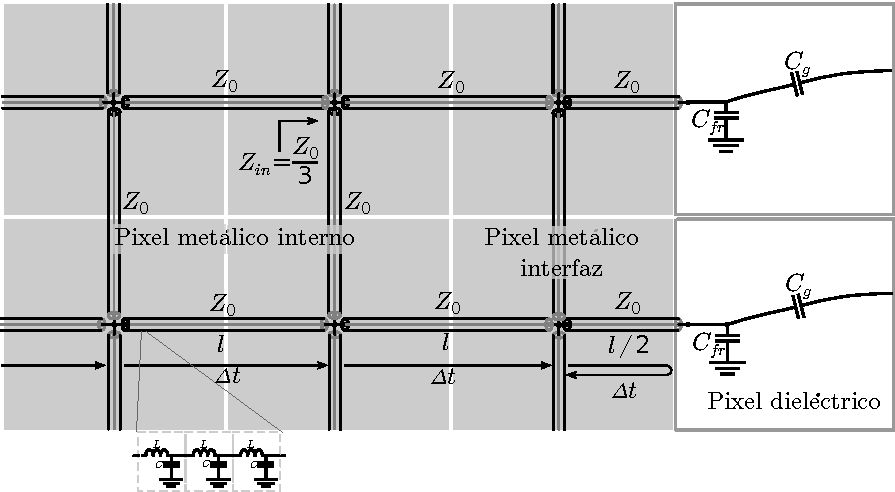
\includegraphics[width=0.8\textwidth]{Modelado/Modelo-Pixeles.pdf}
	\caption{Circuito equivalente de líneas de transmisión, donde se observa la relación con la capacidad e inductancia de cada \textit{Pixel}.}
	\label{fig:modelo-con-lineas-de-transmision}
\end{figure}

Los pixeles interfaz poseen, además, una capacidad de \textit{fringe}, que se relaciona al comportamiento no-TEM de las líneas de campo cerca de los bordes de las estructuras \textit{microstrip}, mostrado en la figura \ref{fig:microstrip-campos}. La expresión de la capacidad de \textit{fringe} para cada borde es la siguiente \cite{ThummWiesbeck:CharacteristicImpedance}, donde $u$ es la profundidad de metal para ese borde en cuestión, como se muestra en la figura \ref{fig:profundidad-para-cfringe}:

\begin{equation}
	C_{fr} = \frac{\epsilon_0 \epsilon_r} {\pi} \ln (2 \pi e^{\frac{u}{2 h} + 0.92})
\end{equation}

\begin{figure}[h]
	\centering
	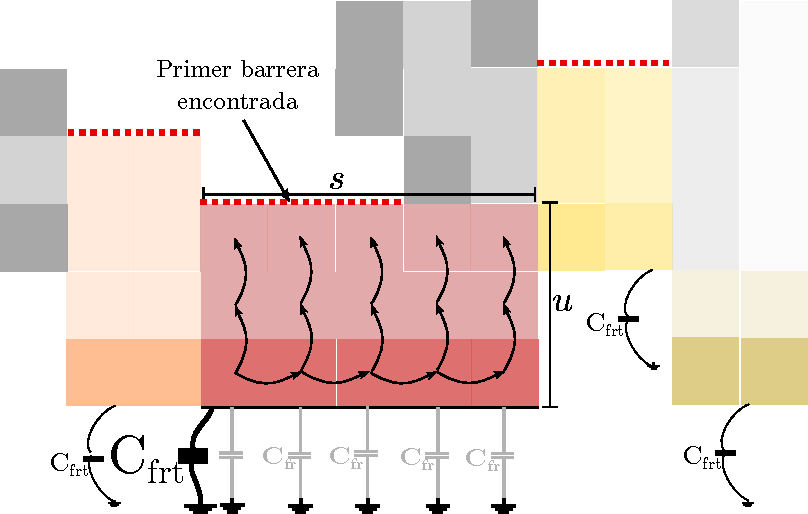
\includegraphics[width=0.8\textwidth]{Modelado/ProcesoCfringe.pdf}
	\caption{Cálculo de la capacidad de \textit{fringe} de una pared horizontal.}
	\label{fig:profundidad-para-cfringe}
\end{figure}

Al momento de crear la superficie, además, se realizan dos acciones previas a la simulación:

\begin{enumerate}
	\item \textbf{Vincular capacitivamente los bordes de las estructuras metálicas}, como se indica en la figura \ref{fig:calculoCapacidadTLM}. Para esto se toman todos los bordes de las estructuras metálicas (los pixeles de tipo \textit{Interfaz}), y se recorre horizontal y verticalmente la matriz, una vez por dirección, vinculando los bordes interfaz de a pares, teniendo en cuenta que aquellos \textit{pixeles} de interfaz que corresponden a la misma estructura (a la misma isla metálica) no deben ser vinculados.
	
	\begin{figure}[h]
		\centering
		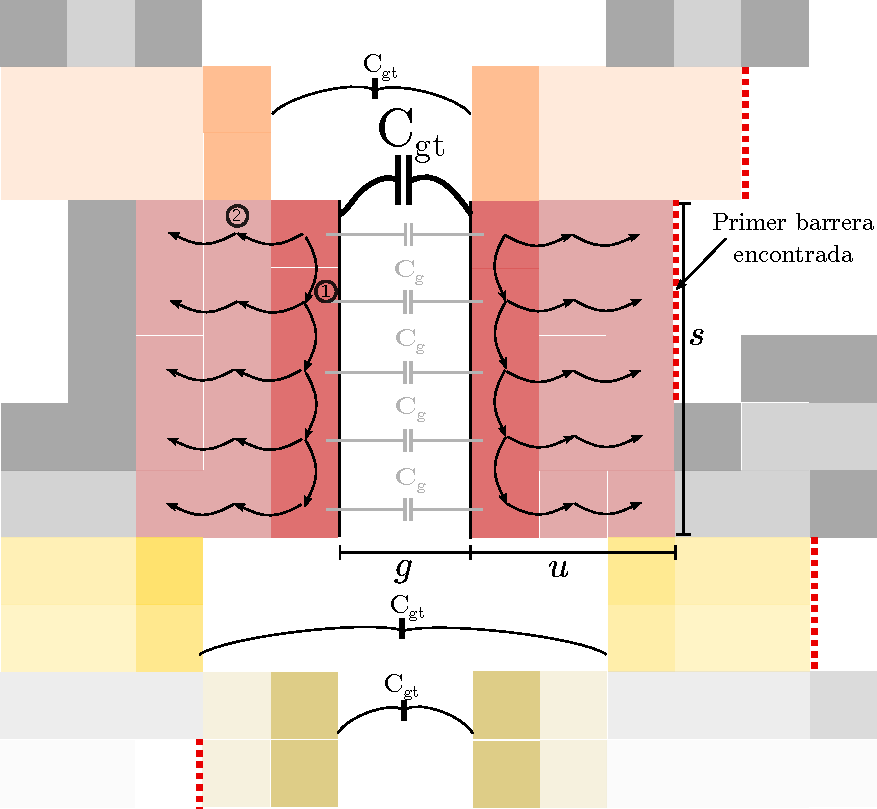
\includegraphics[width=0.9\textwidth]{Modelado/ProcesoProfundidad.pdf}
		\caption{Cálculo de las distintas capacidades de acople horizontales para los pixeles que participan del cálculo numérico. Para un caso particular se muestran las capacidades de acople asociadas a los pixeles enfrentados por un \textit{gap}.}
		\label{fig:calculoCapacidadTLM}
	\end{figure}
	
	Por cada par encontrado, se obtiene la capacidad de acople, $C_{gt}$, utilizando la expresión \ref{eq:cgap-y-lgap}, reescrita aquí con los nombres de los parámetros definidos en esta sección, para simplificar la lectura:
	
	\begin{align*}
		C_{gt} = \frac{b \epsilon_0 (1+\epsilon_r)}{\pi} \cosh^{-1} (a / g) \\
	\end{align*}
	
	En esta expresión, $a$ es el tamaño de las islas metálicas y $g$ representa la distancia entre las islas conductoras. El valor de $s$, en tanto, representa la longitud del $gap$, que se obtiene calculando la cantidad de \textit{pixeles} enfrentado a distancia constante que existen (paso 1 en la figura). Hecho esto, considerando todos los pixeles a uno y otro lado del \textit{gap}, se busca la "profundidad" de la celda, $u$, que no es más que la cantidad de pixeles metálicos detrás de los pixeles frontera que pueden hallarse simultáneamente a ambos lados del \textit{gap}, manteniendo al cantidad longitudinal de pixeles metálicos del borde (paso 2 en la figura). Así, el valor de $a$ queda representado por, aproximadamente, $2*u+g$, con $u$ en unidades de metro.
	
	El valor de la capacidad total de acople se divide entre la cantidad de pares de pixeles que participan del cálculo, de manera que a cada par se le asigna una capacidad $C_g$, como se indica en la figura para los pixeles de color rojo.
	
	\item \textbf{Calcular las matrices S asociadas a cada pixel metálico.} Las matrices S son las matrices que, multiplicadas por un vector de tensiones incidentes, $V_i$ a cada pixel, devuelven un vector de igual cantidad de componentes de tensiones reflejadas, $V_r$, en los mismos, como se muestra en la ecuación \ref{eq:multiplicacion-matriz-s} y en la figura \ref{fig:esquema-matriz-s}. Cada uno de los elementos de estos vectores representan una dirección (izquierda, derecha, arriba y abajo) de la celda unitaria. Las expresiones de la matriz S son las mostradas en la ecuación \ref{eq:matriz-s-expresiones}:
	
	\begin{align}
		\label{eq:multiplicacion-matriz-s}
		\begin{bmatrix}
			V_r^{izq} \\
			V_r^{der} \\
			V_r^{arr} \\
			V_r^{aba} \\
		\end{bmatrix}
			=
		\begin{bmatrix}
			s_{izq-izq} & s_{der-izq} & \dots & \dots \\
			s_{izq-der} & s_{der-der} & \ddots & \vdots \\
			\vdots & \ddots & \ddots     & \vdots \\
			s_{izq-izq-aba} & \dots & \dots & s_{aba-aba}
		\end{bmatrix}
		\begin{bmatrix}
			V_i^{izq} \\
			V_i^{der} \\
			V_i^{arr} \\
			V_i^{aba} \\
		\end{bmatrix}
	\end{align}
	
	\begin{subequations}
		\label{eq:matriz-s-expresiones}
		\begin{align}
			S_{i,i} = \frac{(Z_{j}||Z_{k}||Z_{l}) -Z_{i}}{(Z_{j}||Z_{k}||Z_{l}) +Z_{i}} \\
			S_{j,i} = \frac{2 (Z_{j}||Z_{k}||Z_{l})}{(Z_{j}||Z_{k}||Z_{l}) +Z_{i}}
		\end{align}
	\end{subequations}
	
	\begin{figure}[h]
		\centering
		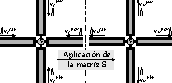
\includegraphics[width=0.9\textwidth]{Modelado/esquema-matriz-s.pdf}
		\caption{Descripción gráfica del uso de la matriz S.}
		\label{fig:esquema-matriz-s}
	\end{figure}
	
	Se debe tener en cuenta que, para el caso de las líneas de transmisión que unen \textit{pixeles} metálicos (\textit{internos} y de \textit{interfaz}), como se muestra en la figura \ref{fig:modelo-con-lineas-de-transmision}, cada una de las 4 líneas de transmisión que confluyen en un nodo representante de un pixel son iguales, por lo que el valor de los elementos de la diagonal de la matriz S será $-0.5$, mientras que los elementos no diagonales valdrán $0.5$.
	
	Además, se pueden establecer pérdidas para el transporte de tensión de un \textit{pixel} a otro, de manera que se puedan simular, de forma simplificada, las pérdidas por conductividad.
	
	Los \textit{pixeles} de tipo \textit{dieléctrico} no poseen matriz S, debido a que en su mayoría no tendrán información de tensión incidente.
\end{enumerate}

% explicar cómo se calcula cuando hay fringe
% explicar el acoplamiento

Para el análisis de transferencia entre un punto y otro de la estructura, se debe fijar una posición de entrada y una posición de salida, cuya tensión, para cada tiempo, deberá ser almacenada.

Una vez creada la matriz a partir de la información obtenida de la imagen, se debe establecer una tensión inicial en el nodo de entrada. Se puede establecer un $\delta(t)$ de tensión, de manera que se fija el valor de tensión inicial y luego se lo deja libre para todos los tiempos posteriores. También puede establecerse un seno, un coseno elevado y un pulso Gaussiano. Estos dos últimos permiten una excitación limitada en frecuencia \cite{Barthia:Handbook}.

La simulación es de tipo TLM, donde existe una tensión inicial impuesta para $t=0$, y elegida previamente al cálculo. A partir de la tensión ubicada en uno de los nodos, se calcula, en cada tiempo discreto, el valor de las tensiones incidentes a cada nodo, y a partir de las mismas, se calculan las tensiones reflejadas en todas las direcciones (\textit{scattering}), sumándose los efectos en todas ellas.

Así, como se muestra en la figura \ref{fig:procedimiento-tlm}, si se inicia el cálculo en el nodo denominado $a$, se impondrá una tensión inicial en el mismo, que será la que se transmita a los nodos adyecentes ($t_{1_b}$), denominados $b_i$. Esta tensión será recibida por los nodos $b_i$, quienes multiplicarán las tensiones incidentes en todas las direcciones (en el tiempo $t_{2_a}$, los nodos $b$ sólo tienen una dirección de incidencia) por su matríz $S$ asociada, para obtener las tensiones reflejadas y transmitidas. Estas tensiones, en el tiempo siguiente ($t_{2_b}$) son las que se transmiten a los respectivos nodos adyacentes, $c_j$, quienes repetirán la operación. El cálculo proseguirá hasta que se interrumpa la simulación.

\begin{figure}[h]
	\centering
	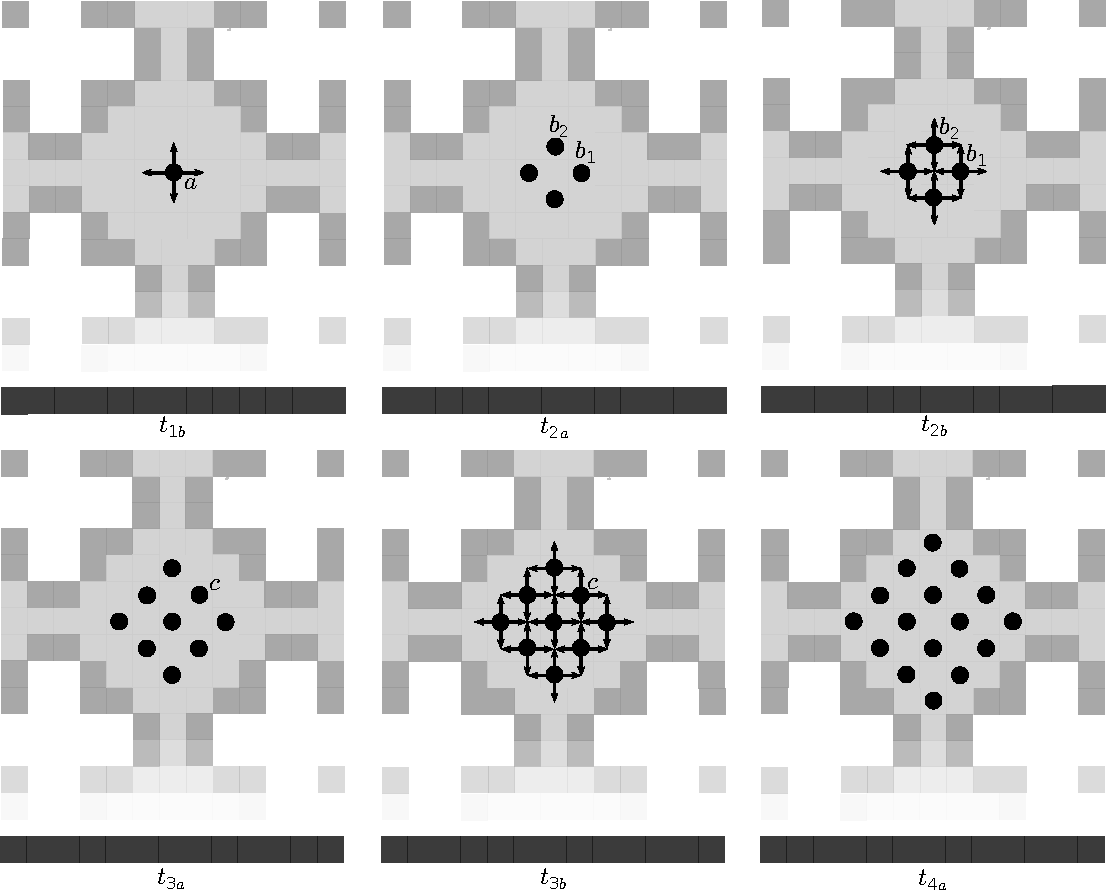
\includegraphics[width=0.9\textwidth]{Modelado/TLM-progresion.pdf}
	\caption{Proceso de cálculo en el dominio del tiempo.}
	\label{fig:procedimiento-tlm}
\end{figure}

Para el caso particular de los \textit{pixeles} de tipo \textit{interfaz}, existen dos situaciones especiales: La correspondiente al efecto de la capacidad de \textit{fringe} y el truncamiento de la línea de transmisión, y el correspondiente al acoplamiento con otras estructuras de la \textit{Superficie}.

Dado que el análisis es cuasiestático, debido a las dimensiones pequeñas de los \textit{gaps} y los Pixeles en comparación con la longitud de onda, se puede utilizar un modelo de bajas frecuencias de acoplamiento mutuo para describir el fenómeno de acoplamiento entre islas metálicas distintas. Este acoplamiento, en términos generales, se da por fenómenos inductivos y capacitivos al mismo tiempo. Si se considera que existe un elemento fuente y un elemento víctima del acoplamiento, se puede afirmar que cada uno de ellos expone una capacidad y una inductancia al ambiente, que son excitadas por los circuitos cercanos. El acoplamiento inductivo se debe a la inductancia mutua $M$ entre las inductancias expuestas de ambos, relacionada al campo magnético presente, mientras que el acoplamiento inductivo se debe a la capacidad de acople entre los circuitos ($C_{g}$).

En términos generales, dado que los \textit{pixeles} y las estructuras son pequeñas y no están conectadas al plano de tierra, en general no existirá un acoplamiento inductivo notorio. Sí se presentará, debido a la cercanía entre las islas metálicas, un acoplamiento capacitivo de mayor magnitud. En vistas de simplificar los cálculos, y bajo estas consideraciones prácticas, será este el tipo de acoplamiento que se analizará, mostrado en la figura \ref{fig:acoplamiento-capacitivo-modelo}.

\begin{figure}[h]
	\centering
	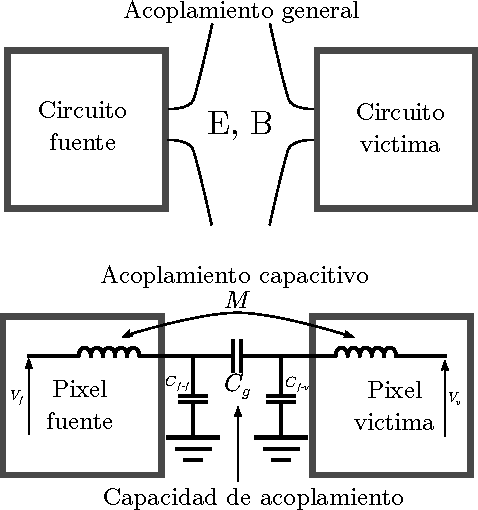
\includegraphics[width=0.5\textwidth]{Modelado/AcoplamientoCapacitivoGeneral.pdf}
	\caption{Modelo de acoplamiento capacitivo entre dos \textit{pixeles}.}
	\label{fig:acoplamiento-capacitivo-modelo}
\end{figure}


En el mismo sentido, debido a que el efecto capacitivo de placas planas paralelas enfrentadas (relacionado a la capacidad de \textit{fringe}) es mucho mayor al de placas planas paralelas coplanares (relacionada a la capacidad entre islas metálicas cercanas), se puede considerar que el acoplamiento es de tipo capacitivo débil \cite{Tesche:EMC} (donde no se considerarán efectos de re-acoplamiento y acoplamiento inverso), lo que permite utilizar un modelo simplificado de acoplamiento, considerando fuentes controladas de corriente, mostrado en la figura \ref{fig:circuito-equivalente-acoplamiento-capacitivo-debil}. Los valores de las fuentes controladas se muestran en la ecuación \ref{eq:expresiones-fuentes-controladas}, aunque en términos prácticos el valor de $M$, la inductancia mutua, se despreciará, por lo que no existirá una fuente controlada de tensión.

\begin{subequations}
	\label{eq:expresiones-fuentes-controladas}
	\begin{align}
		i' = j \omega C_g v_f \\
		v' = j \omega M i_f \approx 0
	\end{align}
\end{subequations}

\begin{figure}[htp]
	\centering
	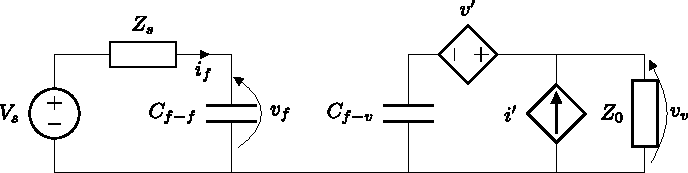
\includegraphics[width=0.8\textwidth]{Modelado/AcoplamientoCapacitivoDebil.pdf}
	\caption{Circuito equivalente del modelo de acoplamiento capacitivo débil, utilizando fuentes de corriente, para una carga de impedancia igual a la impedancia característica de la línea de transmisión conectada.}
	\label{fig:circuito-equivalente-acoplamiento-capacitivo-debil}
\end{figure}

Para adaptar este circuito al modo de funcionamiento de TLM, es posible considerar a la fuente de corriente y el capacitor de \textit{fringe} como un equivalente Norton, y convertirlo en un equivalente Thévenin, de modo que la tensión desarrollada sobre $Z_0$, y por lo tanto, la tensión transmitida al nodo correspondiente al \textit{pixel} víctima, resulte de un divisor de impedancias:

\begin{align}
	v_{th} & = i' \frac{1}{j\omega C_{f-v}} = \frac{j\omega C_g v_f}{j\omega C_{f-v}} = \frac{C_g v_f}{C_{f-v}} \\
	v_v & = v_{th} \times \frac{Z_0}{Z_0 + \frac{1}{j\omega C_{f-v}}} = v_f \frac{C_g}{C_{f-v}} \frac{Z_0}{Z_0 + \frac{1}{j\omega C_{f-v}}}
\end{align}


% Podría haber un delay?

La tensión $v_f$ es la que desarrolla el capacitor de \textit{fringe} del \textit{pixel} fuente. Utilizando consideraciones similares, el efecto de este capacitor para el circuito fuente se podría obtener, para el acoplamiento capacitivo, como el paralelo de la capacidad de \textit{fringe} fuente con el circuito que lo conecta al circuito víctima. Sin embargo, dado que, como se dijo antes, la capacidad $C_g$ es mucho menor a las capacidades de \textit{fringe}, $C_{f}$, los efectos del circuito víctima y de la capacidad de acople son despreciables. De esta forma, el valor del coeficiente de reflexión, para el caso del acoplamiento capacitivo analizado, resulta sólo generado por la capacidad de \textit{fringe} del circuito fuente:

\begin{align}
	\rho =   \frac{|1/(j\omega C_{f-f})| - Z_0}{|1/(j\omega C_{f-f})| + Z_0}
\end{align}

Se debe tener en cuenta que, dado que la señal recorre un camino de $\Delta l / 2$ desde el nodo hasta el capacitor de \textit{fringe}, el cálculo de la tensión reflejada se debe realizar en $n\Delta t/2$. Esto es porque en el tiempo siguiente, exactamente un $\Delta t$ luego de enviada la señal, la tensión reflejada debe impactar en el nodo original, como se esquematizó sobre el \textit{pixel} metálico de la figura \ref{fig:modelo-con-lineas-de-transmision}.

El resultado arrojado por la simulación será un archivo, de formato \textsc{.npy}, que es una matriz tridimensional, que puede ser considerada como un apilamiento, de altura igual a la cantidad de tiempos simulados, de matrices bidimensionales con largo y ancho iguales a los de la estructura, como se muestra en la figura \ref{fig:EstructuraTiemposMatrizNumpy}. En cada una de estas matrices bidimensionales, cada elemento posee un valor, que no es más que la tensión vista en ese nodo en el tiempo $t_k$ al que corresponde la altura $k$ en que se evalúa la matriz bidimensional. De ser necesario, se pueden establecer los parámetros de una ventana de Hanning para disminuir el comportamiento espúreo de alta frecuencia debido a la limitación en tiempo de la señal de salida.

\begin{figure}[h]
	\centering
	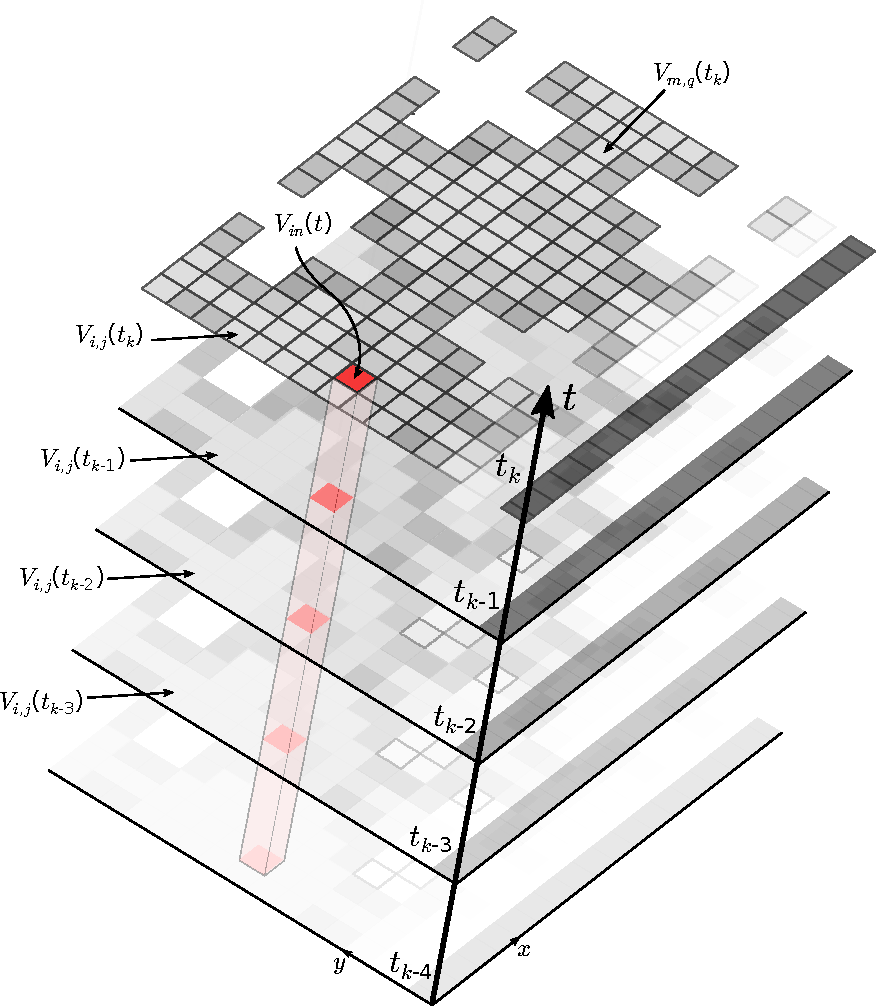
\includegraphics[width=0.9\textwidth]{Modelado/ConceptoMatrizProgresoTiempo.pdf}
	\caption{Estructura de la matriz que se guarda y se lee del disco rígido. La estructura posee todas las tensiones calculadas para cada tiempo y para cada pixel en particular.}
	\label{fig:EstructuraTiemposMatrizNumpy}
\end{figure}

El análisis de la tensión del nodo de salida, teniendo en cuenta la tensión del nodo de entrada aplicada, da lugar a una transferencia de tensión.